\documentclass{hedlectures}
\usepackage[russian]{babel}
\usepackage[utf8]{inputenc}
\usepackage[derivative,vectors,environments]{hedmaths}
\usepackage{graphicx}
\usepackage{multirow}

%-------------colors for links---------------------------

\usepackage{color}
\definecolor{darkgreen}{rgb}{0,.5,0}
\usepackage[colorlinks,linkcolor=black,filecolor=blue,citecolor=darkgreen]{hyperref}

%--------------------------------------------------------

\title{Векторный и тензорный анализ}
\author{Лекции Михайлова~В.~К.}

%--------------------------------------------------------
\begin{document}
    \maketitle
    \tableofcontents
    \setlength{\parskip}{0.2cm}
    \parindent=0cm
    \section{Понятие о скалярных, векторных и тензорных величинах}

\subsection{Скаляры}

    Скаляр -- физическая или математическая величина, которая описывается числом или функцией. Скаляр инвариантен относительно преобразований координат. Примерами скаляров являются
    \begin{itemize}
        \item масса \( m \); 
        \item потенциал \( \phi = \phi(x, y, z) \);
        \item работа \( A \);
        \item температура \( T = T(x, y, z, t) \);
        \item давление \( P = P(x, y, z, t) \).
    \end{itemize}

subsection{Векторы}

    Вектор, в отличие от скаляра, характеризуется не одним, а тремя независимыми числами:
    \[ \vec{a} = \{ a_{x}, a_{y}, a_{z} \}. \]

    Однако, не все тройки чисел являются векторами. Так например вектором не является тройка \( (P,\ V,\ T) \), так как одна из величин связана с двумя другими при помощи уравнения состояния.
    
    Векторами являются такие физические величины, как
    \begin{itemize}
        \item скорость \( \vec{v} = \{v_x(x, y, z),\ v_y(x, y, z),\ v_z(x, y, z)\} \);
        \item сила \( \vec{F} = \{F_x(x, y, z),\ F_y(x, y, z),\ F_z(x, y, z)\} \);
        \item напряжённость электрического поля \( \vec{E} = \vec{E}(x, y, z) \).
    \end{itemize}

\subsection{Тензоры}

    Тензор является более общим понятием, чем скаляр. Тензор, в зависимости от своего ранга, характеризуется \( 3^n \) числами. Для нас тензор будет характеризоваться \( 3^2 \), \( 3^3 \) и \( 3^4 \) числами.
    
    Тензоры появляются в ситуациях, когда требуется описать какое-либо явление, происходящее в неоднородной среде. Рассмотрим для примера закон Ома.
    
    Если среда изотропна, то закон Ома имеет вид \( i = \frac{1}{R} U \).
    
    Запишем его в дифференциальном виде:
    \[ \vec{j} = \lambda \vec{E} \]
    или в проекциях: 
    \begin{equation}
    \left\{ \begin{array}{l}
            j_{1} = \lambda E_{1}, \\
            j_{2} = \lambda E_{2}, \\
            j_{3} = \lambda E_{3};
    \end{array} \right. \label{eq1.1}
    \end{equation}
    где \( \vec{j} \) -- плотность тока, \( \vec{E} \) -- электрическое поле, \( \lambda \) -- удельная проводимость материала (скалярная величина),

    В этом случае вектор \( \vec{j} \) сонаправлен вектору \( \vec{E} \).

    Если среда анизотропна, то вместо (\ref{eq1.1}) надо записать следующее:
    \begin{equation}
        \left\{
        \begin{array}{c}
            j_{1} = \lambda_{11} E_{1} + \lambda_{12} E_{2} + \lambda_{13} E_{3}, \\
            j_{2} = \lambda_{21} E_{1} + \lambda_{22} E_{2} + \lambda_{23} E_{3}, \\
            j_{3} = \lambda_{31} E_{1} + \lambda_{32} E_{2} + \lambda_{33} E_{3}
        \end{array}
        \right.
    \end{equation}
    или 
    \[ j_{k} = \sum\limits_{i=1}^3 \lambda_{ki} E_i, \]
    где \( k = 1,\ 2,\ 3 \).
    
    В матричном виде это будет выглядеть так:
    \[ \vec{j} = \Lambda \vec{E}, \]
    где \( \Lambda \) -- матрица тензора электропроводимости:
    \[ \Lambda =
        \begin{pmatrix}
            \lambda_{11} & \lambda_{12} & \lambda_{13} \\
            \lambda_{21} & \lambda_{22} & \lambda_{23} \\
            \lambda_{31} & \lambda_{32} & \lambda_{33} 
        \end{pmatrix}. \]

    Поэтому в общем случае вектор \( \vec{j} \) неколлинеарен вектору \( \vec{E} \).

    \begin{definition}
        Cреда называется линейной, если её реакция \( y \) связана каким-либо линейным соотношением с воздействием \( X \): \( y = L(X) \).
    \end{definition}
 
    В линейных среда выполняется все линейные законы:
    \begin{itemize}
        \item закон Ома \( i = u/r \), для анизотропной среды: \( \vec{j} = \Lambda \vec{E} \);
        \item закон Гука \( \sigma = \eps E \);
        \item закон Фурье \( \vec{j} = -k \nabla T \).
    \end{itemize}

    Если \( \vec{j} \sim E^2 \), то говорят, что среда нелинейна относительно поля \( \vec{E} \). 

    Пример нелинейных сред:
    \begin{itemize}
        \item ферромагнетики - типичные нелинейные среды, т.к. в них \( \vec{B} \nsim \vec{H} \);
        \item сегнетоэлектрики.
    \end{itemize}
 
    \begin{definition}
        Среда называется однородной, если её свойства одинаковы во всех точках. В противном случае среда называется неоднородной.
    \end{definition}

    \begin{definition}
        Среда называется изотропной, если её свойства в данной точке одинаковы по всем направлениям. В противном случае среда называется анизотропной.
    \end{definition}

    Если предметом векторной алгебры являются алгебраические операции с постоянными векторами, то предметом векторного анализа являются свойства и операции над скалярными и векторными полями, определённые в трехмерном евклидовом пространстве.

\subsection{Понятие об инвариантности свойств объектов}

    Рассмотрим вектор \( \vec{a} = \{a_x, a_y, a_z\} \):
    \begin{figure}[ht]
        \center
        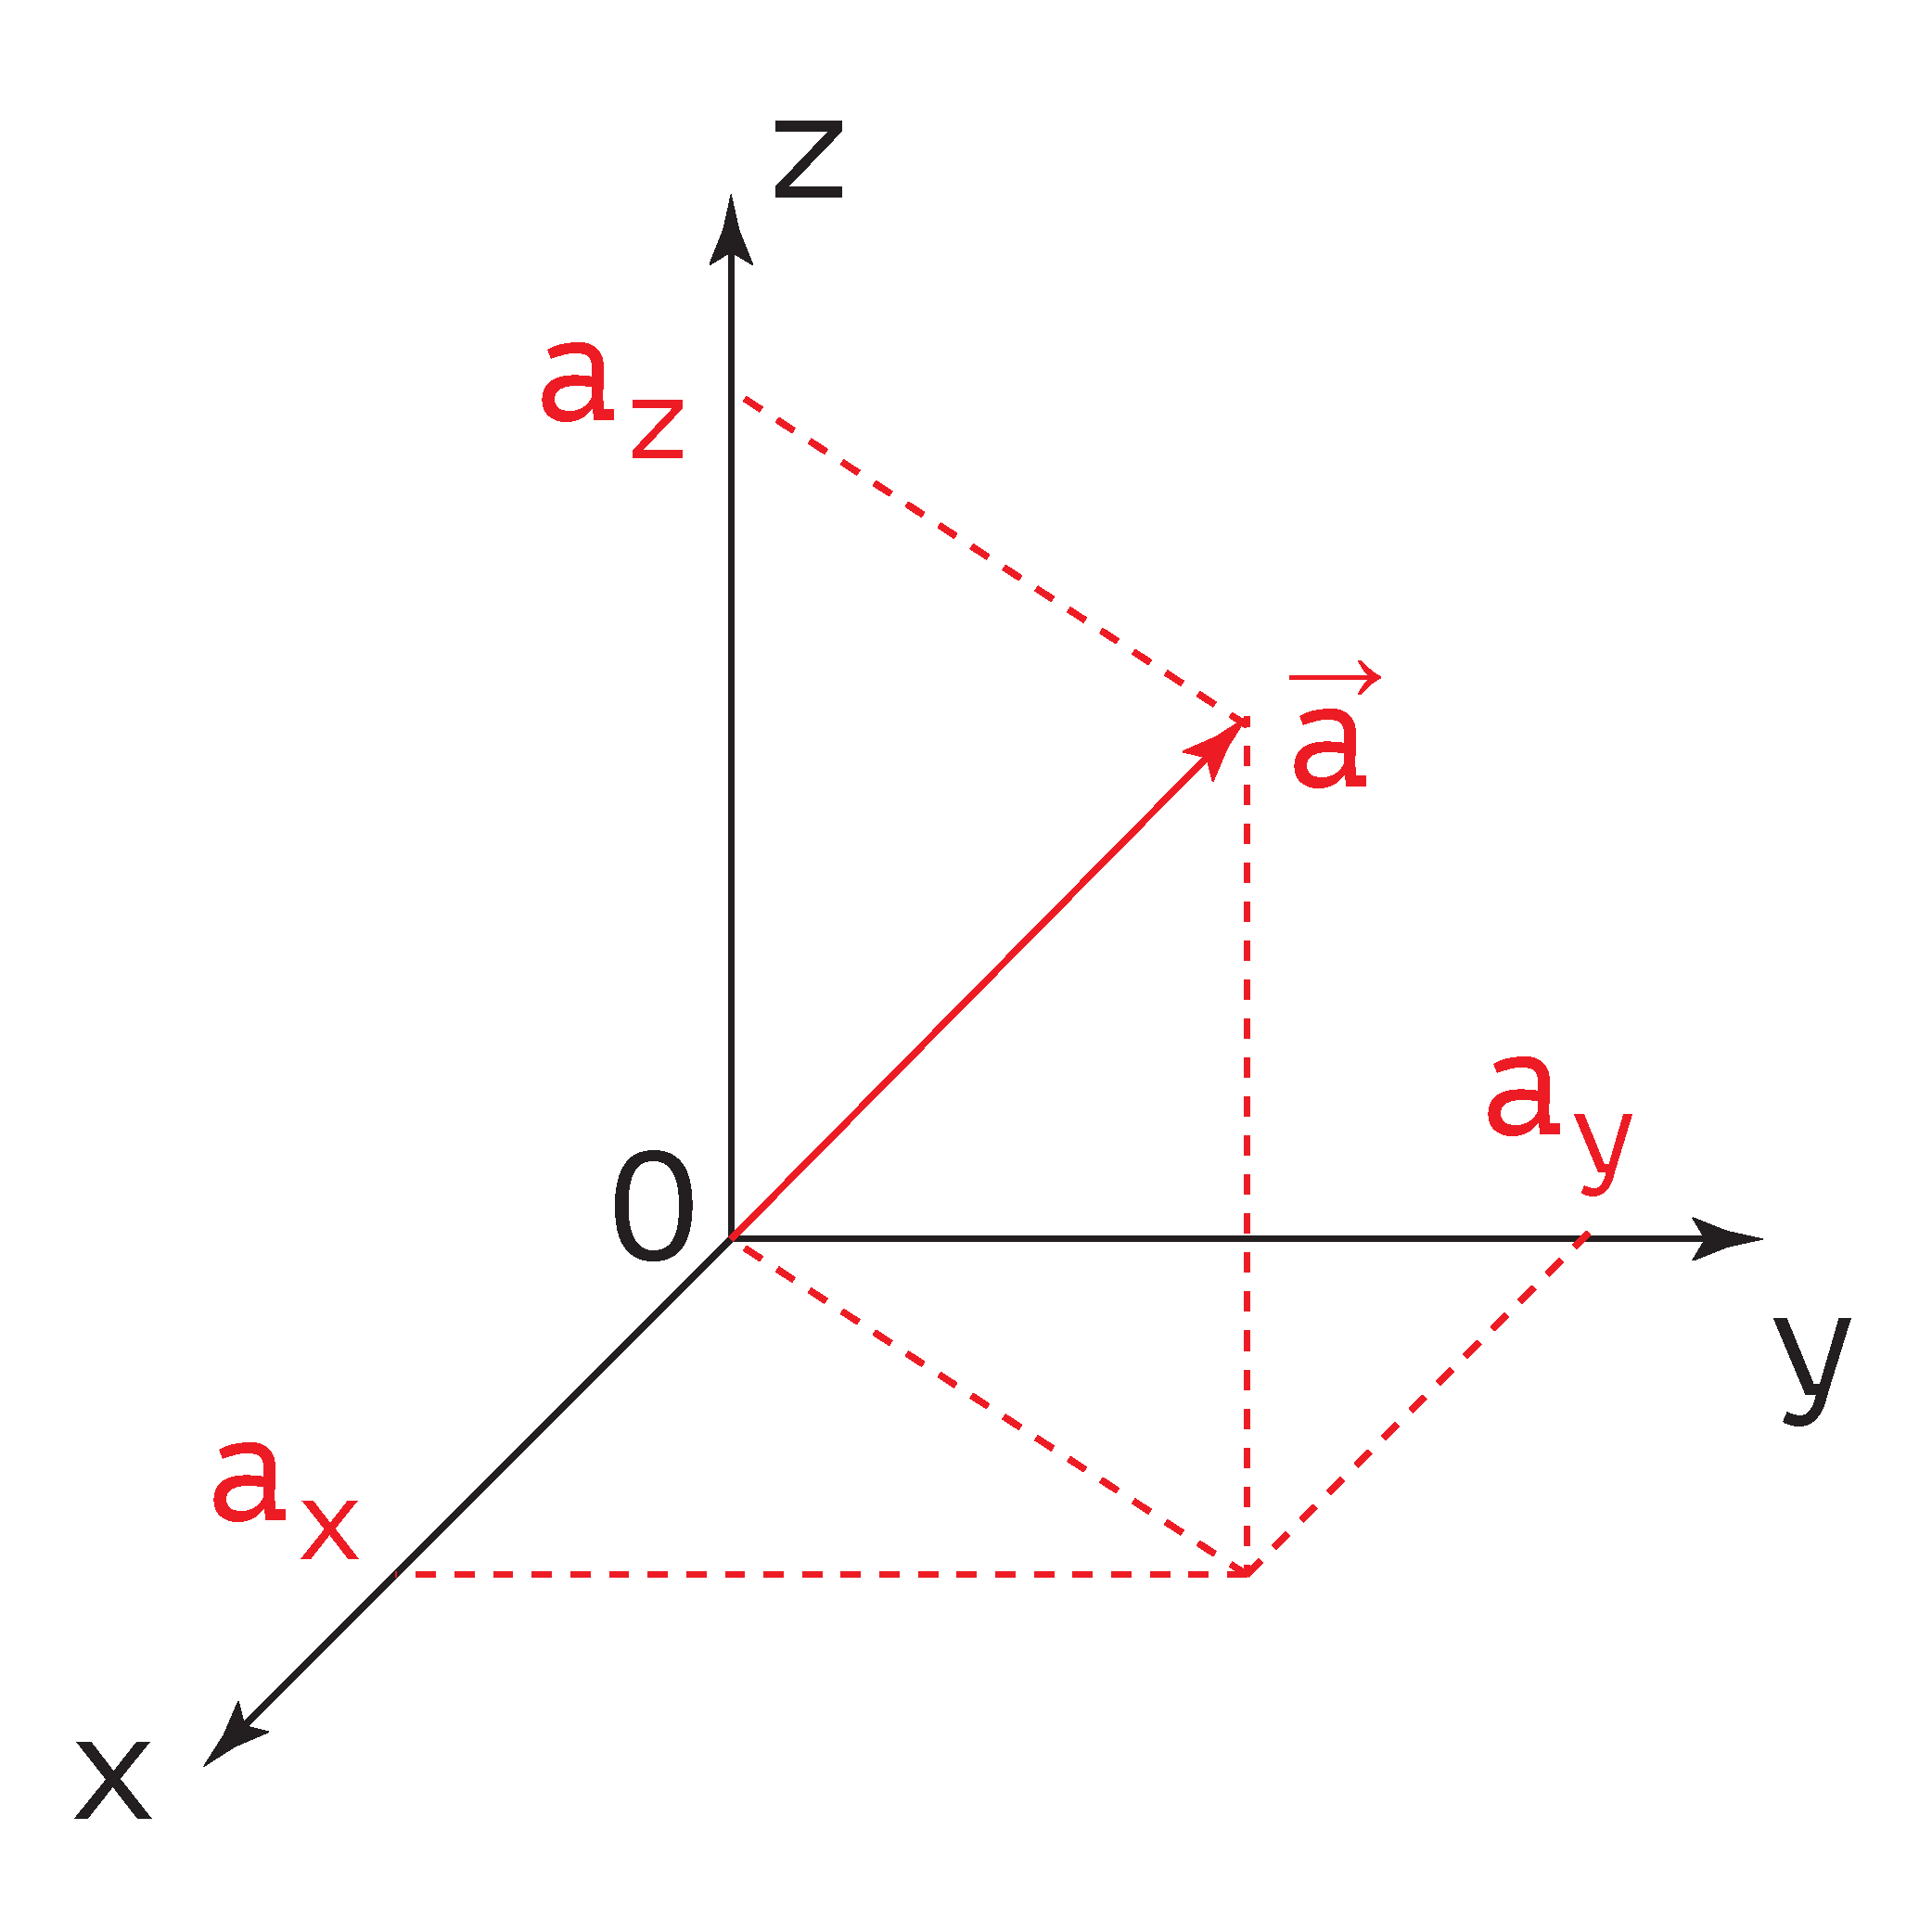
\includegraphics[width=100px]{lec01/vec_a.pdf}
    \end{figure}

    Длина этого вектора может быть найдена как \( |\vec{a}| = \sqrt{a_x^2+a_y^2+a_z^2} \). При поворотах базиса координаты вектора будут претерпевать изменения, однако, длина вектора изменяться не будет.

    \begin{definition}
        Величины или параметры, которые не изменяются при поворотах базиса, называются инвариантными относительно поворотов базиса.
    \end{definition}

    Также к инвариантам можно отнести скалярное произведение векторов \( \vec{a}\cdot\vec{b} \).

    \section{Скалярное поле}

\subsection{Определение}

	\begin{definition}
	Если в каждой точке пространства задана скалярная функция \( u = u(x, y, z) \), то говорят, что в пространстве определено скалярное поле \( u = u(x, y, z) \). При этом предполагается, что функция \( u \) принимает конечные действительные значения.
	\end{definition}
	
	Примеры скалярных полей:
	\begin{itemize}
	\item \( T = T(x, y, z) \) -- поле распределения температур;
	\item \( P = P(x, y, z) \) -- поле давления;
	\item \( \rho = \rho(x, y, z) \) -- поле распределения плотности;
	\item \( \varphi = \varphi(x, y, z) \) -- поле потенциала.
	\end{itemize}
	
	Если \( u = u(x, y, z, t) \), то поле называется нестационарным.

\subsection{Поверхности и линии уровня скалярного поля}

    Геометрическим представлением скалярного поля являются поверхности уровня.

    \begin{definition}
        Поверхность уровня скалярного поля \( u(x,y,z) \) -- это геометрическое место точек в пространстве, для которых выполняется равенство \( u(x,y,z) = \const = C \).
    \end{definition}

    \begin{figure}[h]
        \center
        \begin{minipage}[h]{0.49\textwidth}
        \center{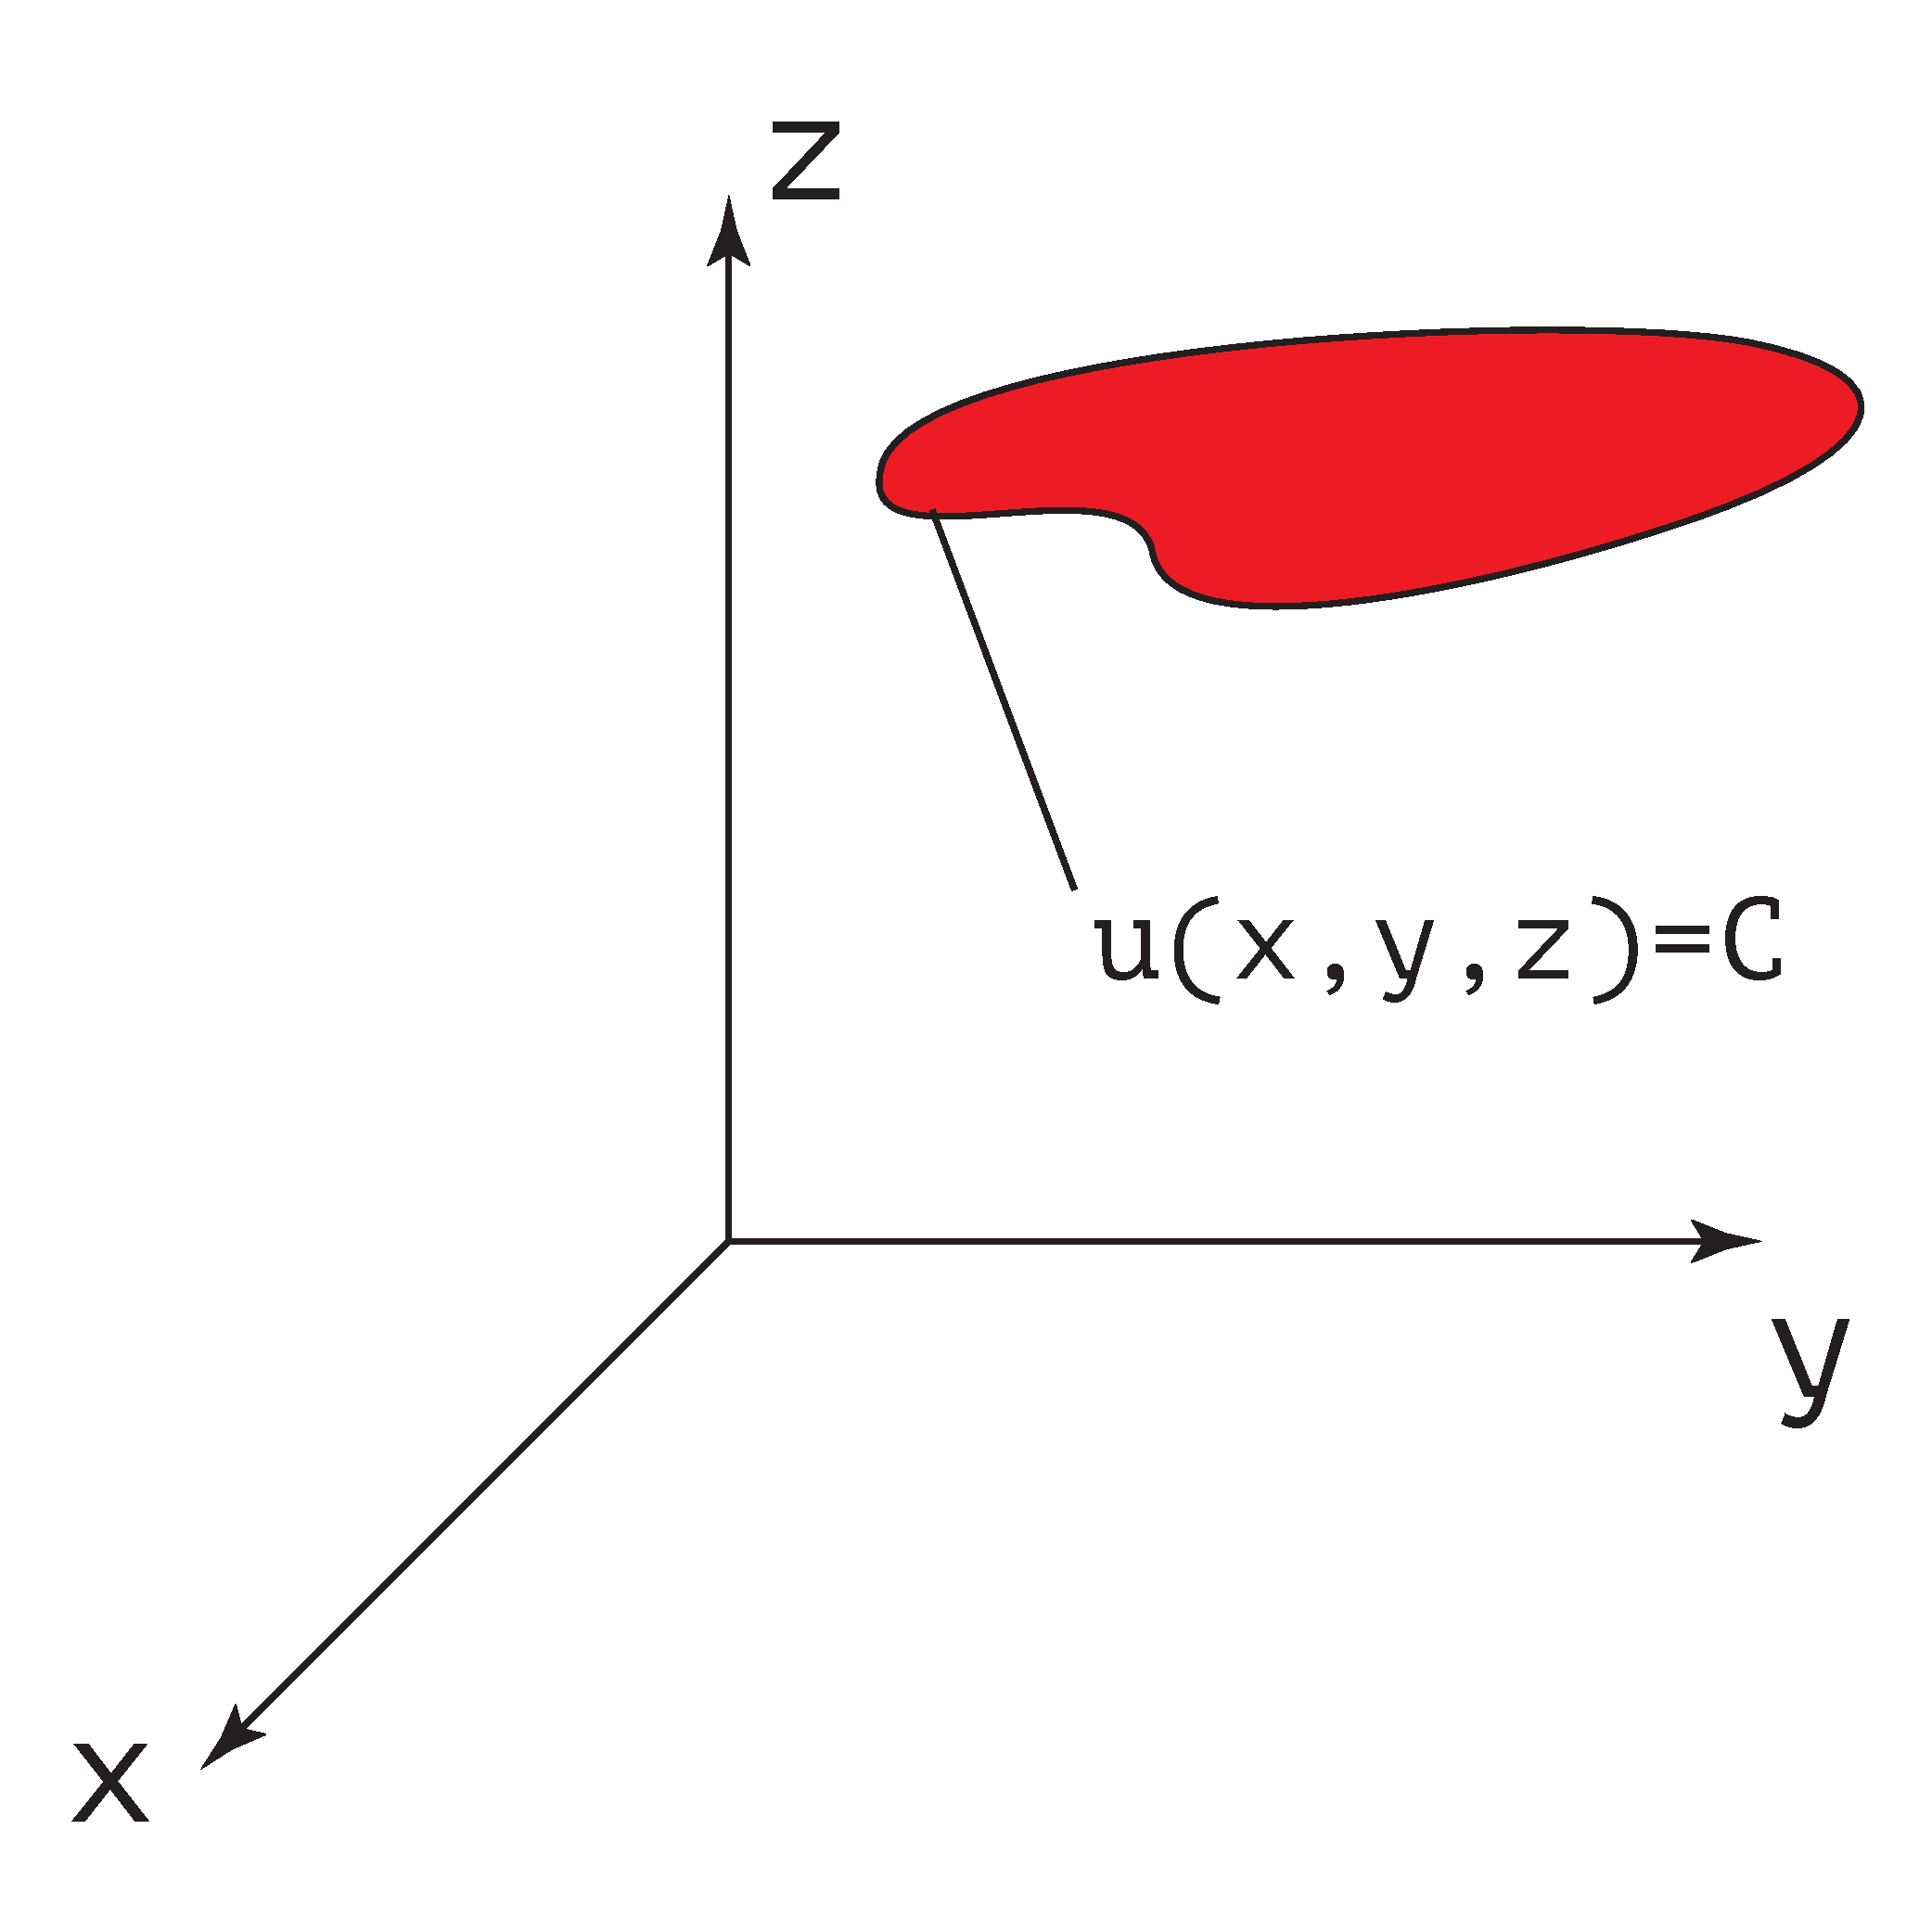
\includegraphics[width=0.47\textwidth]{lec02/surface_of_level.pdf} \\ Поверхность уровня}
        \end{minipage}
        \hfill
        \begin{minipage}[h]{0.49\textwidth}
        \center{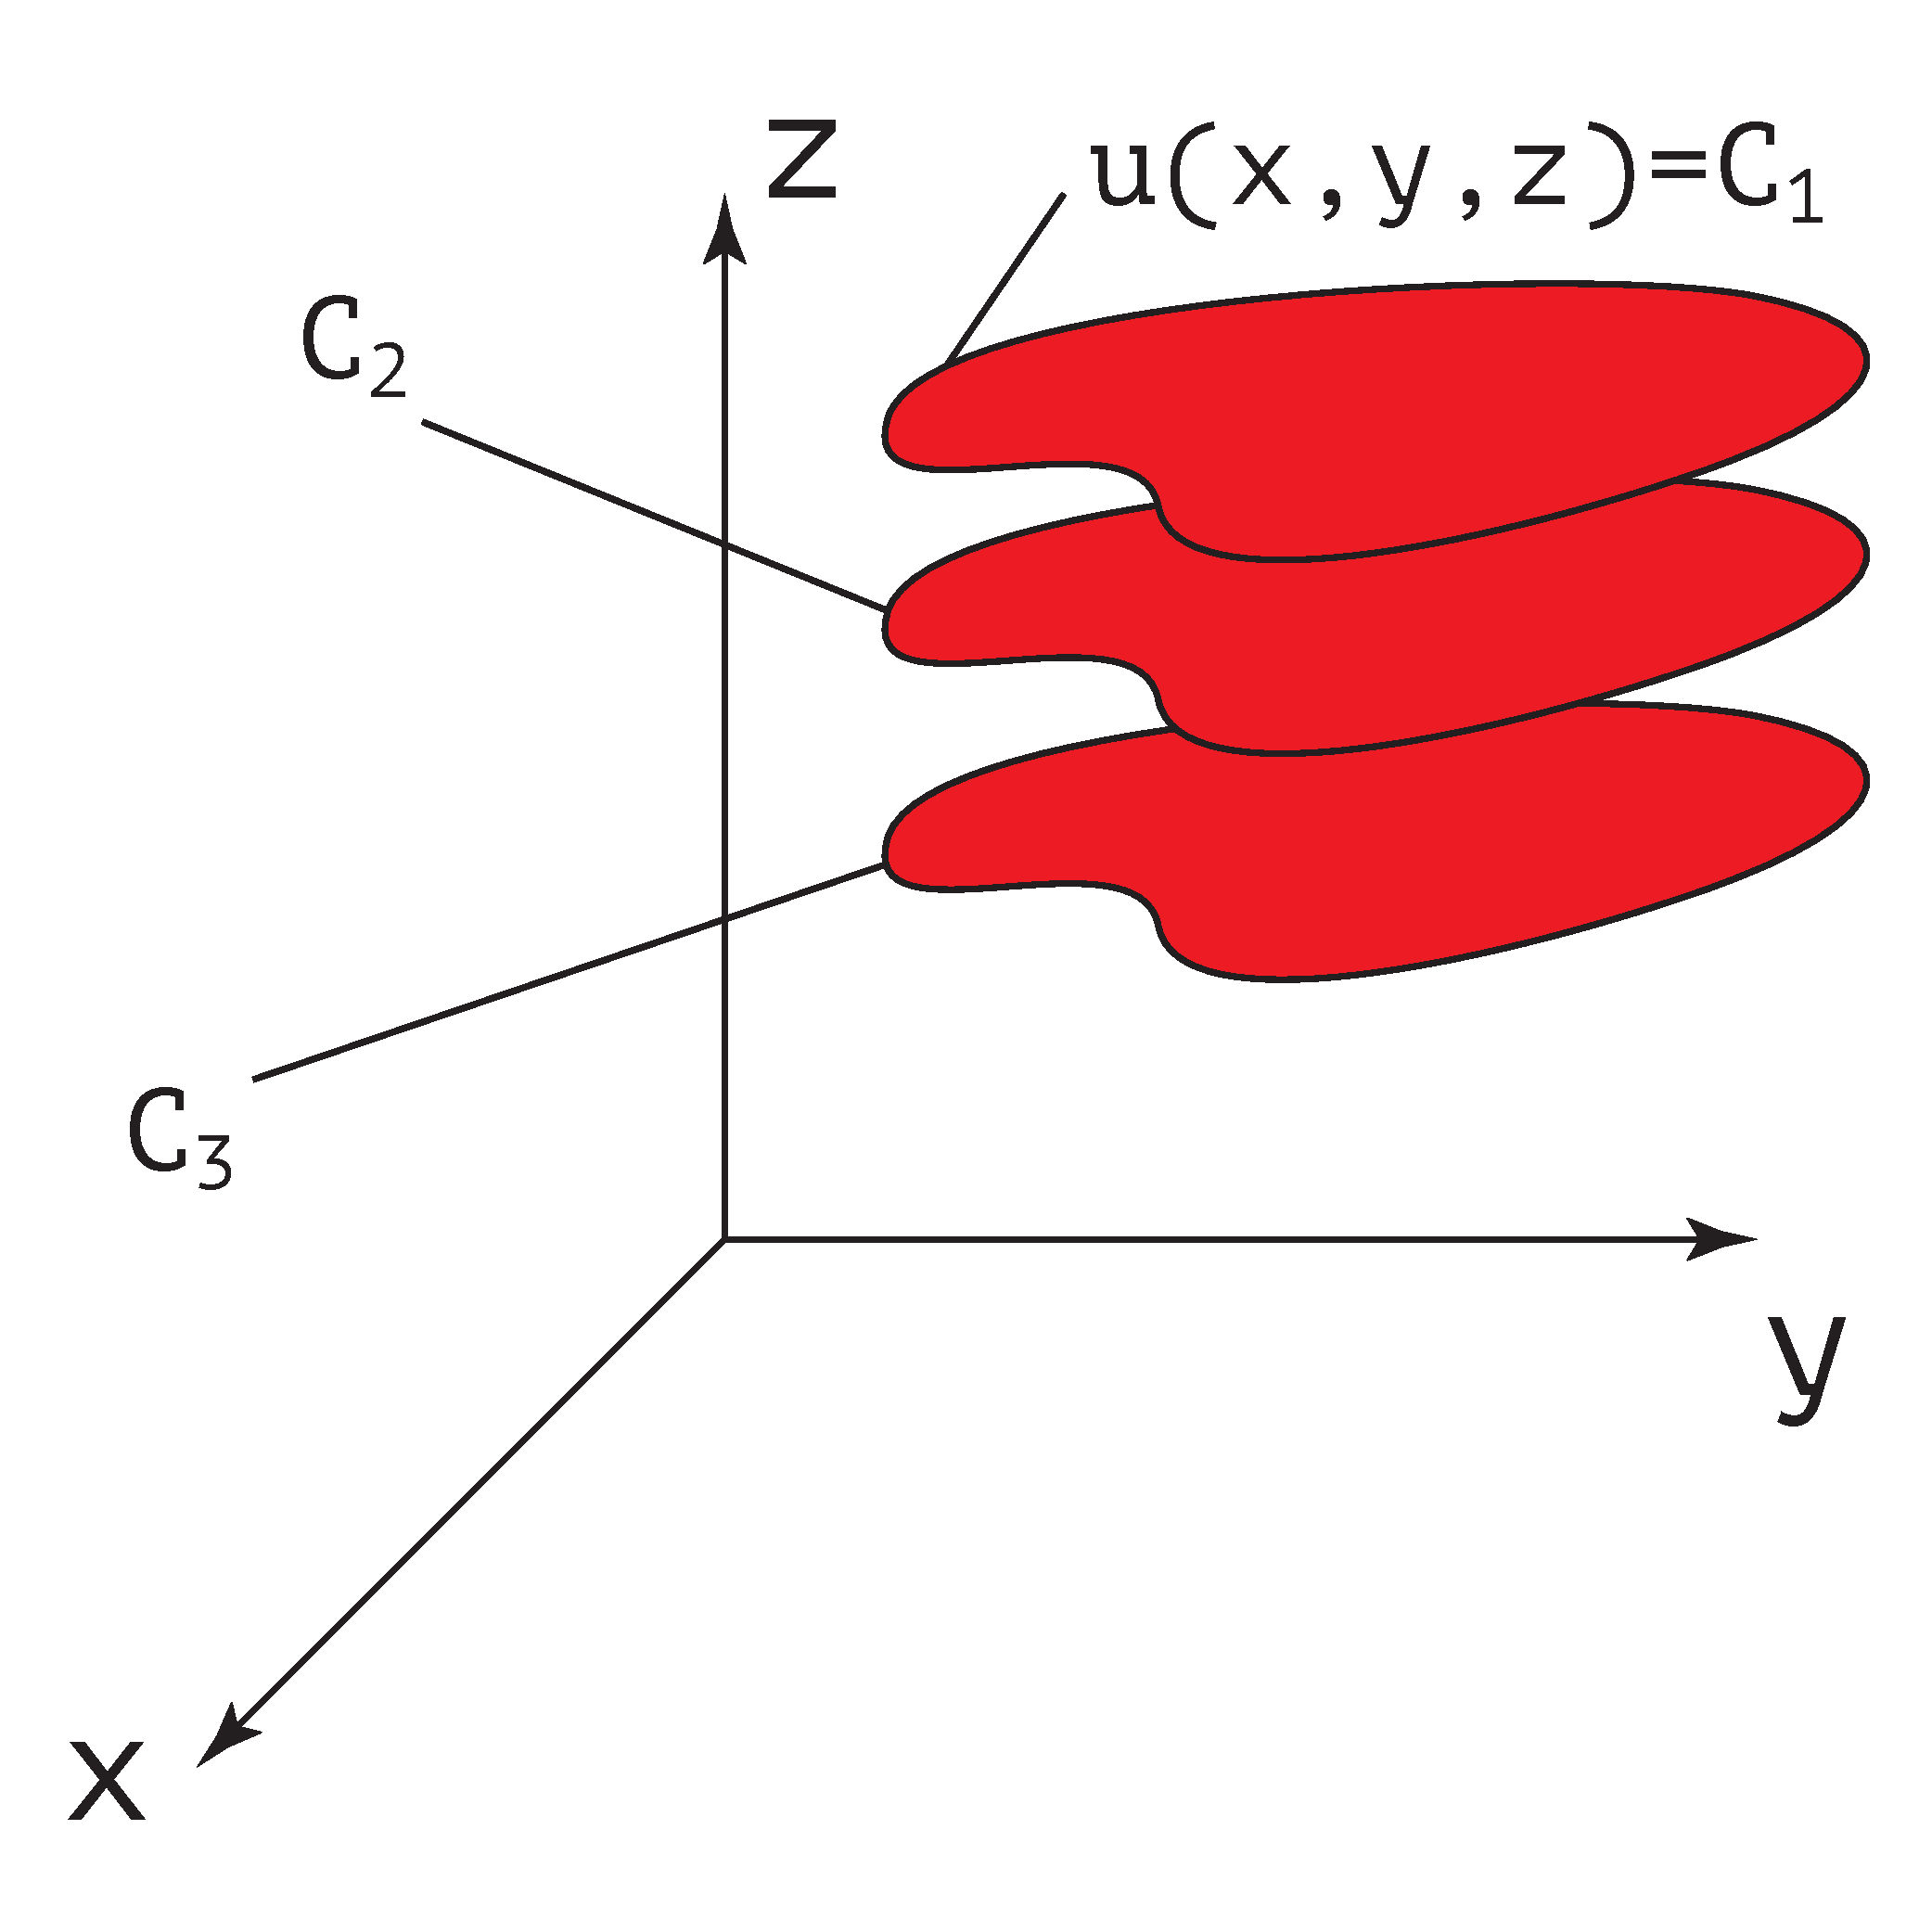
\includegraphics[width=0.47\textwidth]{lec02/family_of_surfaces.pdf} \\ Семейство поверхностей уровня}
        \end{minipage}
        \end{figure}

    \begin{remark}
        Так как \( u(x,y,z) \) по определению однозначна, то поверхности уровня не пересекаются.
    \end{remark}

    \begin{example}
        Поверхностями уровня потенциала точечного заряда являются концентрические сферы.
    \end{example}

    \begin{example}
        Семейством эквитемпературных поверхностей тонкой нагретой нити является система коаксиальных цилиндров.
    \end{example}

    \begin{example}
        Определить поверхности уровня скалярного поля \( u = \vec{a}\cdot\vec{r} \), где \( \vec{a} \) -- постоянный вектор.
    \end{example}

    \begin{solution}
    
    \[ u = a_xx + a_yy + a_zz = C_n. \]
    Это уравнение задаёт семейство плоскостей.
    \end{solution}

    \begin{remark}
        Если функция \( u = u(x,y) \), то поле называется плоским или двумерным, и его геометрическим представлением являются линии уровня на плоскости xOy.
    \end{remark}

    \begin{figure}[h]
        \center
        \begin{minipage}[h]{0.49\textwidth}
        \center{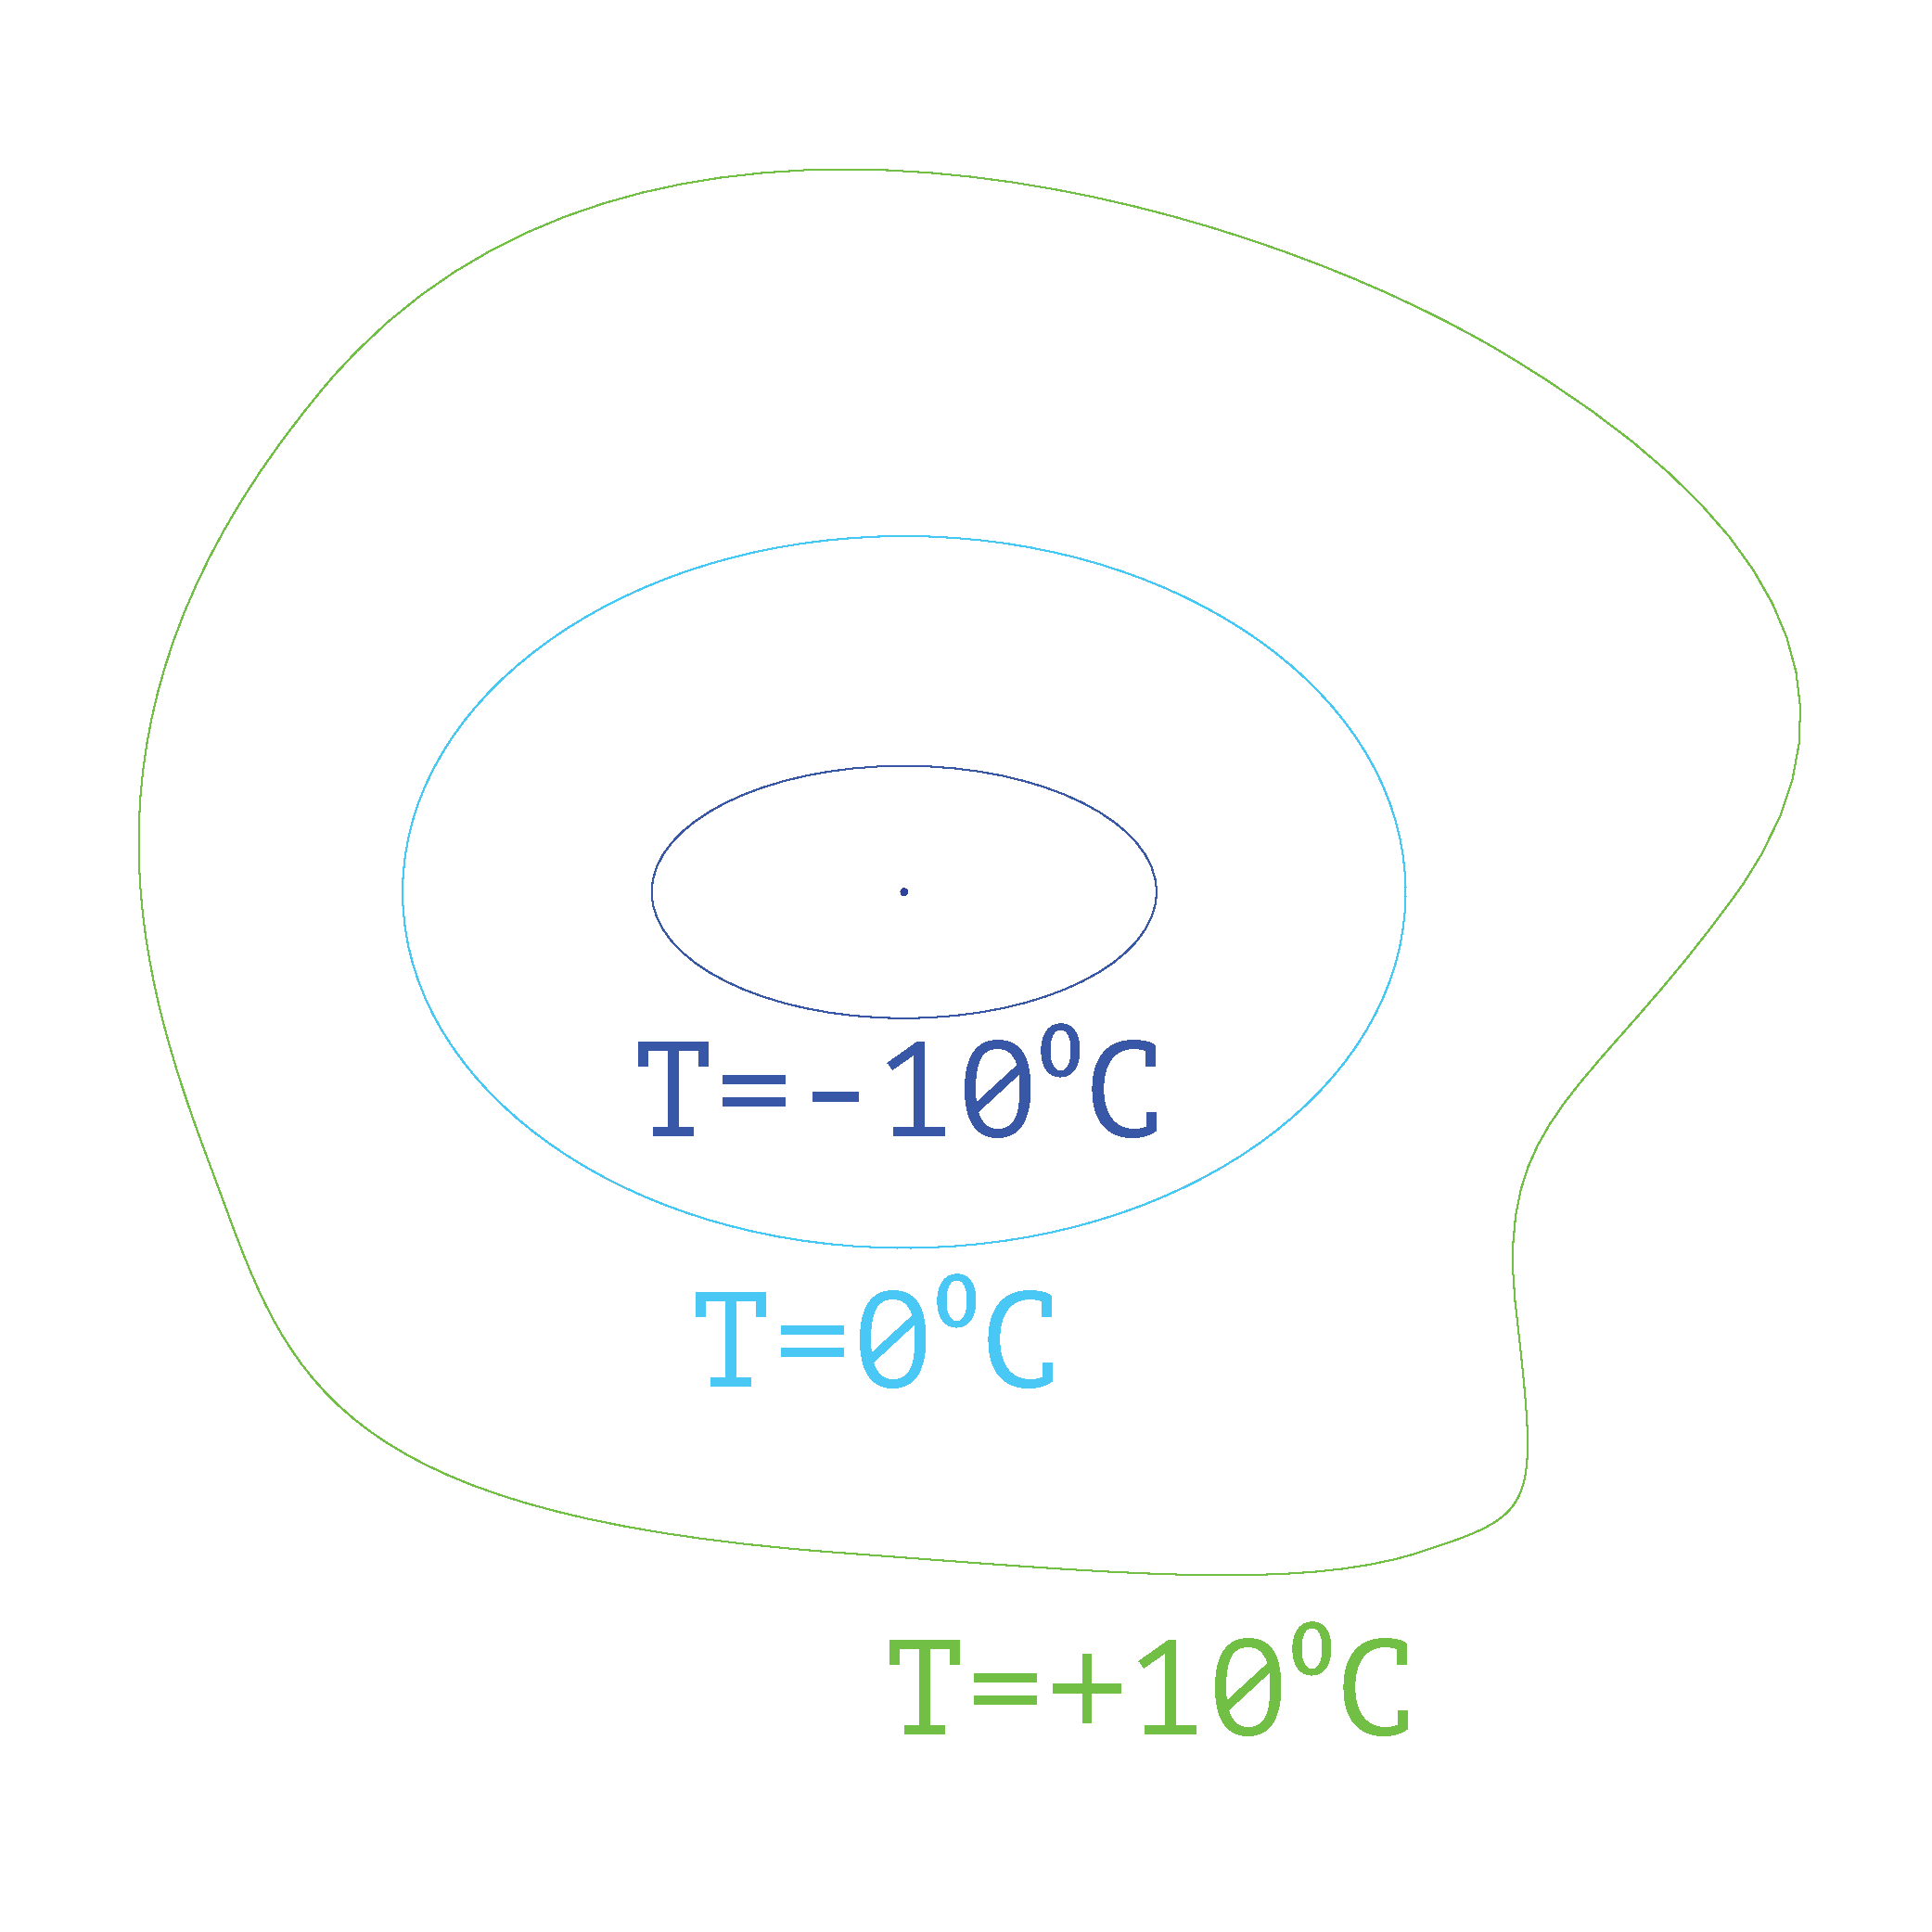
\includegraphics[width=0.47\textwidth]{lec02/temp_lines.pdf} \\ Эквитемпературные линии}
        \end{minipage}
        \hfill
        \begin{minipage}[h]{0.49\textwidth}
        \center{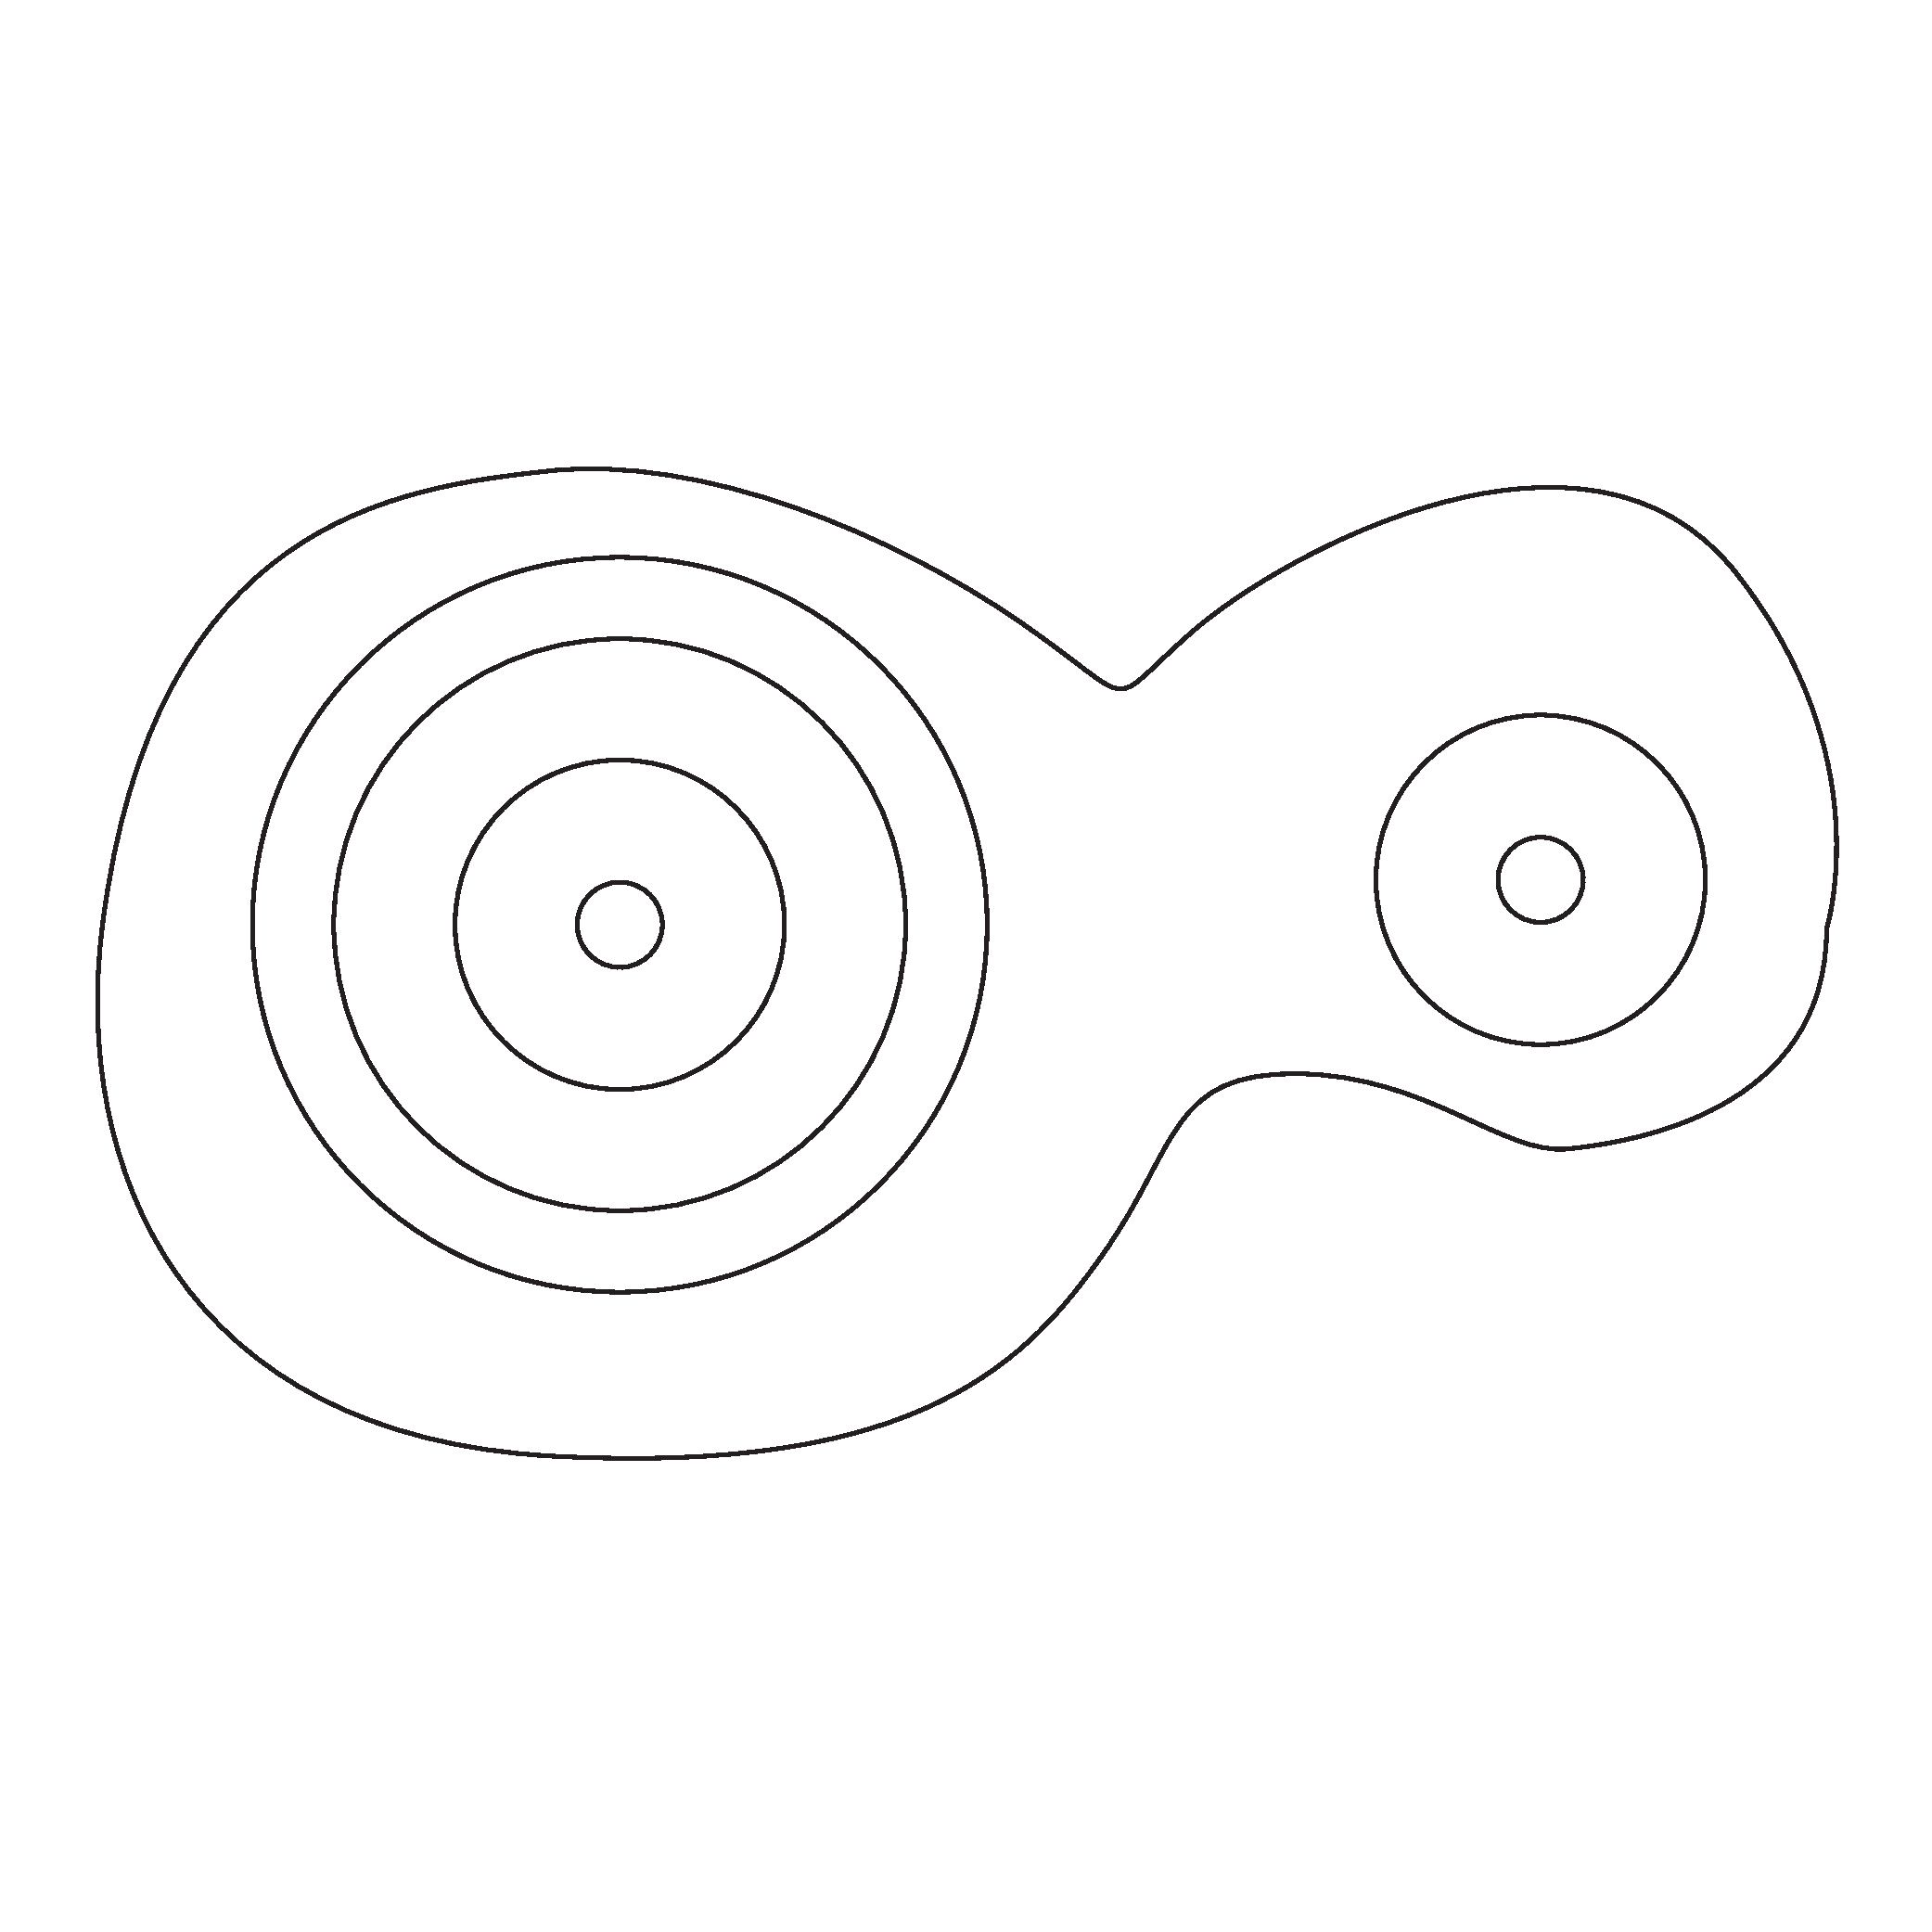
\includegraphics[width=0.47\textwidth]{lec02/height_lines.pdf} \\ Линии равных высот}
        \end{minipage}
    \end{figure}

\subsection{Производная скалярного поля по направлению}

    Пусть задано скалярное поле \( u = u(x,y,z) \). Выберем в нем точку \( M \) и проведём через неё прямую \( l \), задаваемую единичным вектором \( \vec{l} \).

    Составим соотношение:
    \[ \frac{u(M')-u(M)}{MM'}. \]

    Предел этого соотношения
    \[ \lim_{MM'\rightarrow0}\frac{u(M')-u(M)}{MM'} \]
    зависит от направления \( \vec{l} \) -- для \( MM' \) он будет другим в силу \( u(M') = u(M'') \). Этот предел называется производной скалярного поля \( u(x,y,z) \) в точке \( M \) по направлению \( \vec{l} \):
    \[ \der{u}{l} = \frac{u(M')-u(M)}{MM'}. \]
    
    \begin{figure}[h]
        \center
        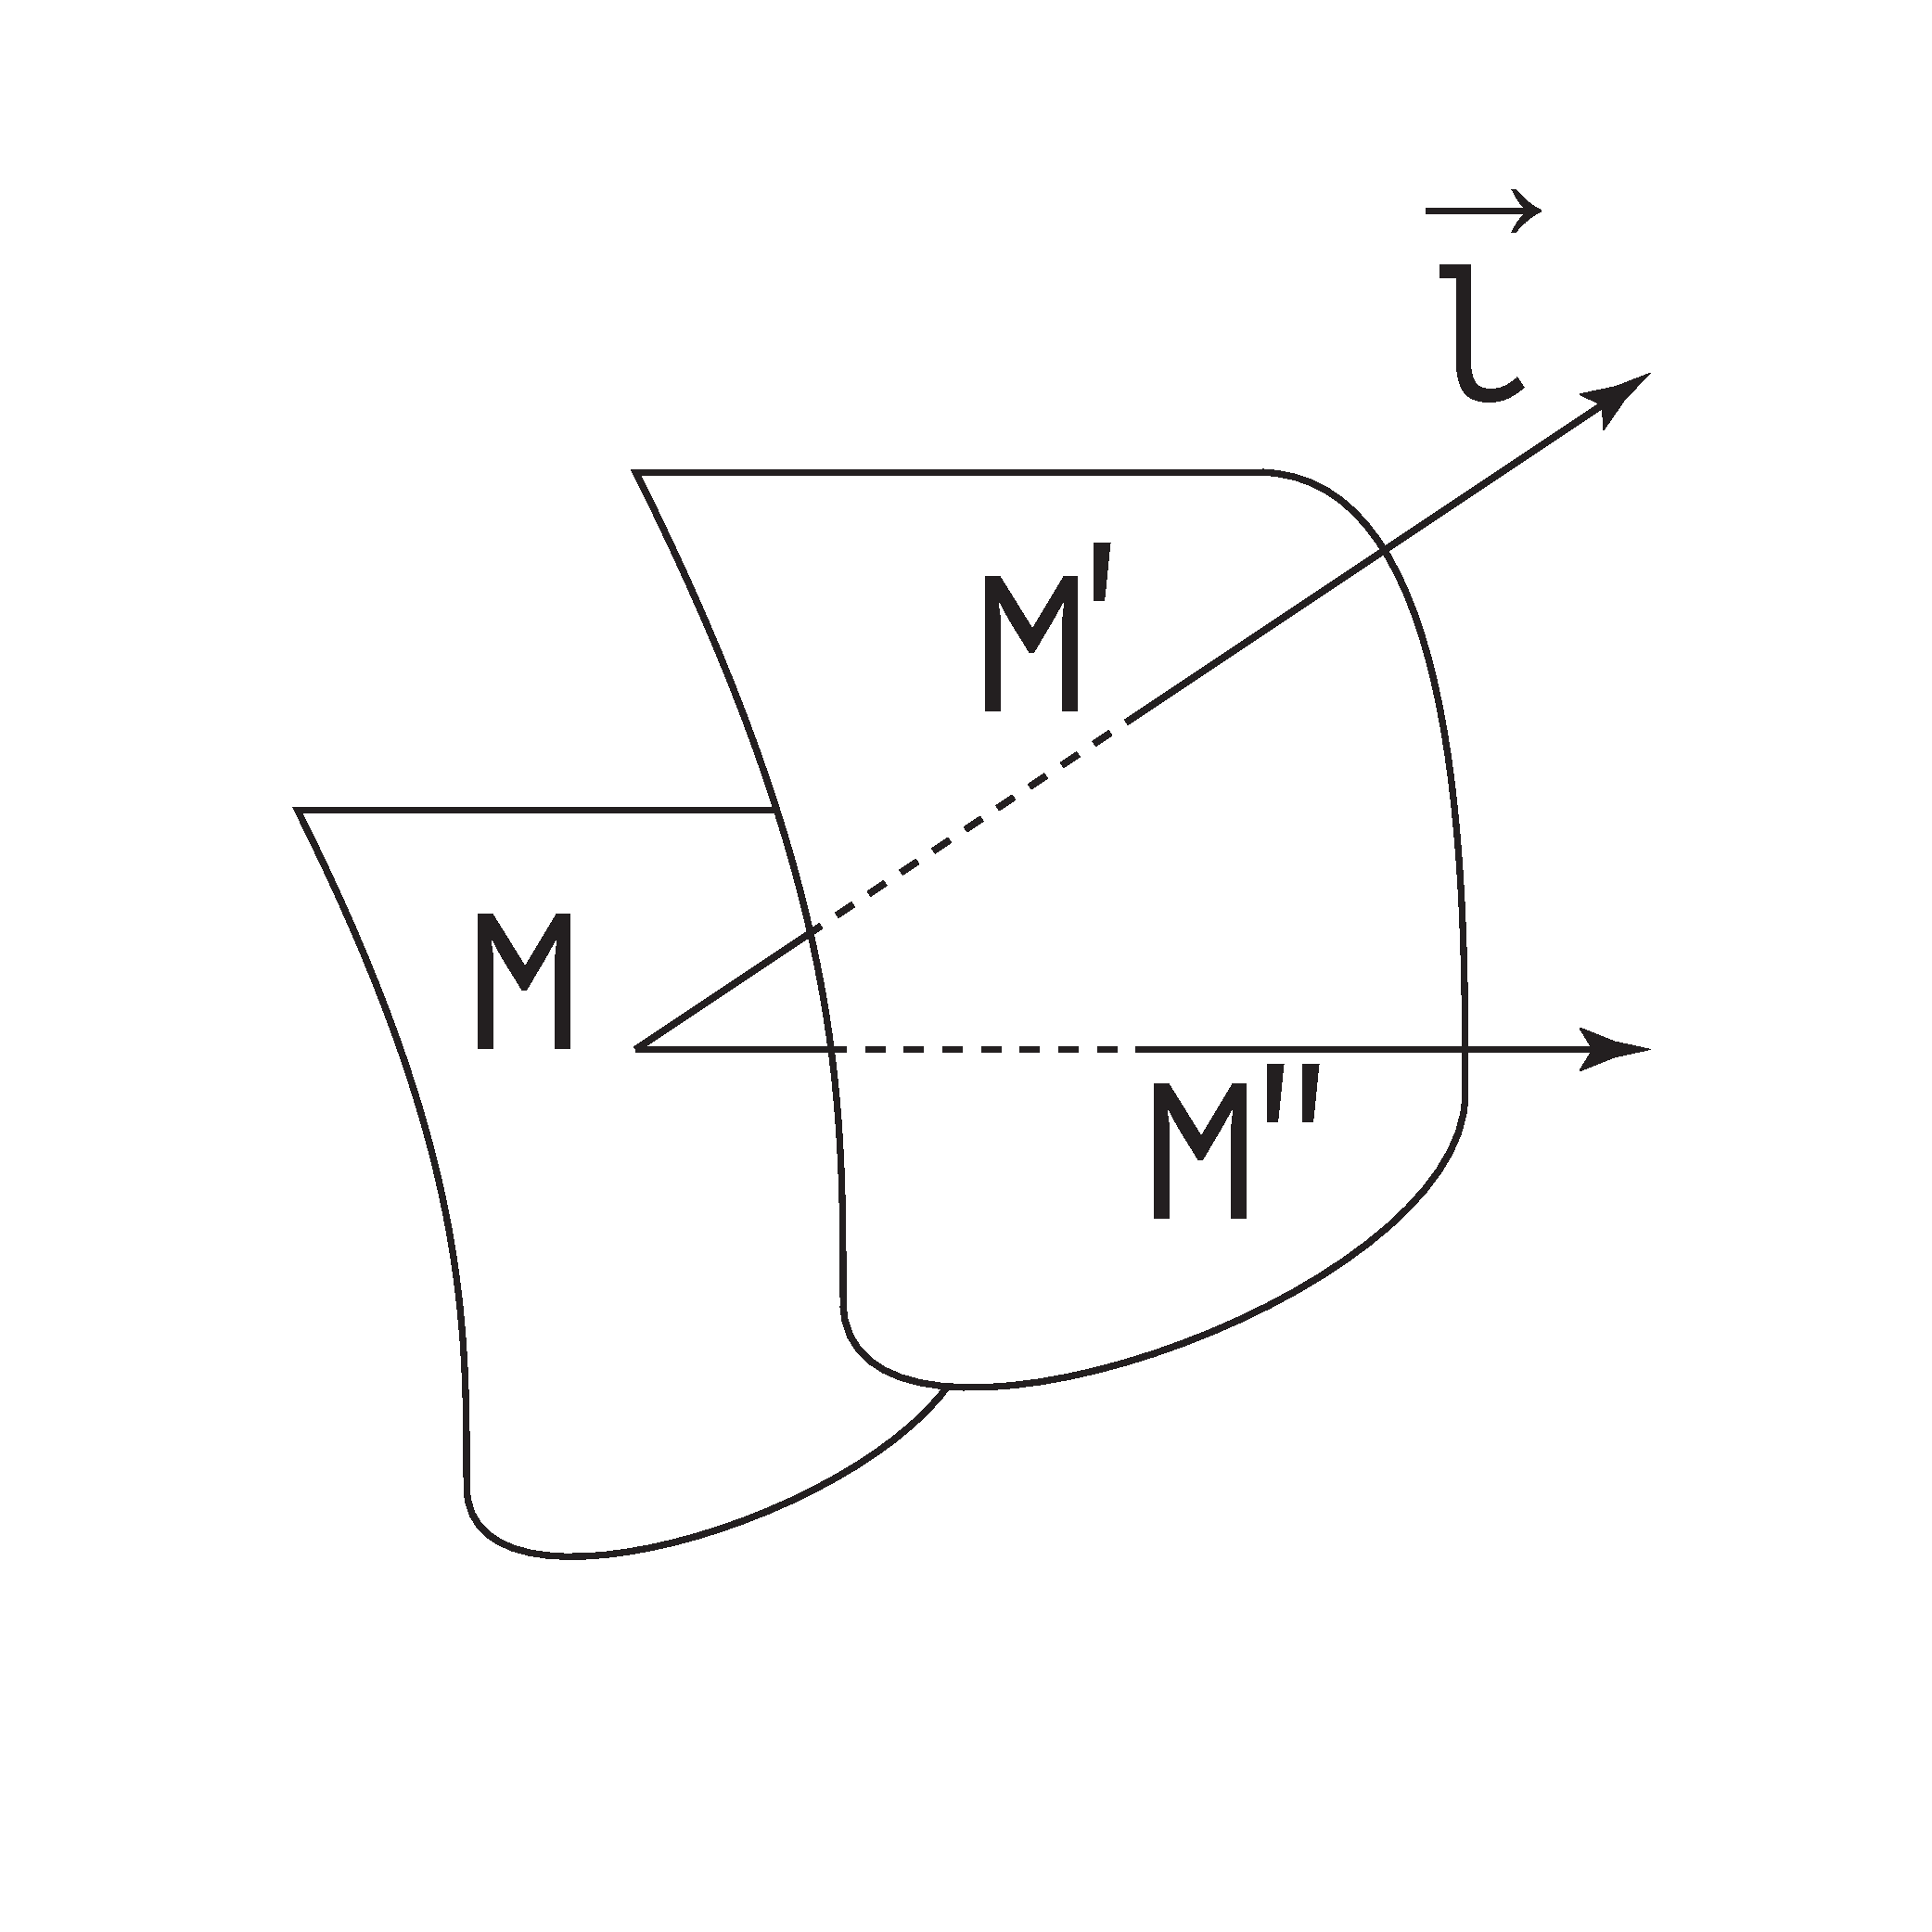
\includegraphics[width=0.47\textwidth]{lec02/derivation_by_direction.pdf}
        \caption{Производная по направлению}
    \end{figure}

    \begin{remark}
        Производная скалярного поля по направлению -- это скаляр.
    \end{remark}

    \begin{remark}
        Производная является инвариантом относительно преобразований базиса.
    \end{remark}

    Чтобы привести выражение для производной к удобной для вычисления форме, запишем его как производную сложной функции:
	\begin{equation}
	\der{u}{l} = \der{u}{x}\cdot\der{x}{l} + \der{u}{y}\cdot\der{y}{l} + \der{u}{z}\cdot\der{z}{l}.
	\label{eq:2.1}
	\end{equation}
    С учётом
    \[ \left\{ \begin{array}{l}
                \der{x}{l} = \frac{l_x}{|\vec{l}|} = l_x = \cos\alpha, \\
                \der{y}{l} = \frac{l_y}{|\vec{l}|} = l_y = \cos\beta, \\
                \der{z}{l} = \frac{l_z}{|\vec{l}|} = l_z = \cos\gamma, \\
            \end{array} \right. \]
    выражение принимает вид:
    \[ \der{u}{l} = \der{u}{x}\cdot\cos\alpha + \der{u}{y}\cdot\cos\beta + \der{u}{z}\cdot\cos\gamma. \]

\subsection{Градиент скалярного поля. Оператор Гамильтона}

    Рассмотрим выражение (\ref{eq:2.1}). Его можно представить как следующее скалярное произведение: \( \vec{l}\cdot\{\frac{\partial u}{\partial x}, \frac{\partial u}{\partial y}, \frac{\partial u}{\partial z}\} \).
    
    Последний вектор называется градиентом скалярного поля \( u(x,y,z) \):
    \begin{equation}
        \gradient u = \left\{\der{u}{x},\ \der{u}{y},\ \der{u}{z}\right\}.
        \label{eq:2.2}
    \end{equation}
    
    Таким образом, выражение (\ref{eq:2.1}) принимает вид:
    \begin{equation}
        \der{u}{l} = \vec{l}\cdot\gradient u.
        \label{eq:2.3}
    \end{equation}
    
    Комбинация производных \( \left\{ \der{}{x},\ \der{}{y},\ \der{}{z}\right\} \) образует символический вектор \( \nabla \) -- оператор дифференцирования, называемый оператором Гамильтона.
    
    Тогда, уравнение (\ref{eq:2.3}) может быть записано в виде:
    \begin{equation}
          \der{u}{l} = \vec{l}\cdot\nabla u. \label{eq:2.4}
    \end{equation}
    
    \begin{remark}
    Уравнение (\ref{eq:2.4}) можно записать в виде
    \begin{equation}
         \der{u}{l} = \left(\vec{l}\cdot\nabla\right)u, \label{eq:2.5}
    \end{equation}
    где \( \vec{l}\cdot\nabla = l_x\der{}{x} + l_y\der{}{y} + l_z\der{}{z} \) -- дифференцирование по направлению.
    \end{remark}
    
    \begin{example}
    Вычислить градиент скалярного поля \( u = \vec{a}\cdot\vec{r} \), где \( \vec{a} = \{ a_x,\ a_y,\ a_z \} = \const \).
    \end{example}    
    
    \begin{solution}
    
    \[ \gradient{u} = \nabla u = \left\{ \der{u}{x},\ \der{u}{y},\ \der{u}{z} \right\} = \{ a_x,\ a_y,\ a_z \} = \vec{a}. \]
    \end{solution}
    
    \begin{example}
    Найти градиент потенциала \( \phi \) поля точечного заряда \( q \): \( \phi = \frac{q}{4\pi\eps_0 r} = k\frac{1}{r} \), где \( r = \sqrt{x^2 + y^2 + z^2} \).
    \end{example}    
    
    \begin{solution}
    
    \[ \nabla\phi = k\nabla\frac{1}{r} = k\{ \der{}{x}\left(\frac{1}{r}\right),\ \der{}{y}\left(\frac{1}{r}\right),\ \der{}{z}\left(\frac{1}{r}\right) \}. \]
    
    Частная производная по \( x \) от \( \frac{1}{r} \):
    \[ \der{}{x}\left(\frac{1}{r}\right) = -\frac{1}{r^2}\cdot\der{r}{x} = -\frac{x}{r^3}. \]
    
    Аналогично, производные по \( y \) и \( z \):
    \[ \begin{array}{l}
	\der{}{y}\left(\frac{1}{r}\right) = -\frac{y}{r^3}; \\
	\der{}{z}\left(\frac{1}{r}\right) = -\frac{z}{r^3}.
    \end{array} \]
    
    Окончательно,
    \[ \nabla\varphi = -k\frac{1}{r^3}\{ x, y, z \} = -k\frac{\vec{r}}{r^3} = -\frac{q\vec{r}}{4\pi\eps_0 r^3} = -\vec{E} \text{ -- электрическое поле} \]
    \end{solution}
% subsection Градиент скалярного поля. Оператор Гамильтона (end)

	\subsection{Свойства градиента}
	\begin{enumerate}
	\item Вектор \( \gradient{u} \) перпендикулярен поверхности уровня \( u(x, y, z) = \const \) в любой его точке.	
	\begin{proof}
	
	Рассмотрим поверхность уровня \( u(x, y, z) =\const \). Пусть \( \vec{l}_\mathrm{\tau} \) касательный единичный вектор к ней в точке \( M \). А так как, по определению поверхности уровня, \( u = \const \), то \( \der{u}{l_\mathrm{\tau}} = \vec{l}_\mathrm{\tau}\cdot\nabla u = 0 \). Следовательно, \( \nabla u \perp \vec{l}_\mathrm{\tau} \) для любого касательного вектора и поверхности уровня в точке \( M \).
	\end{proof}
	
	\item Функция \( u(x, y, z) \) растет вдоль направления \( \nabla u \).
	\begin{proof}
	
	Вычислим производную по направлению градиента \( \nabla u \):
	\[ \der{u}{l} = \vec{l}\cdot\nabla u = |\vec{l}|\cdot|\nabla u| > 0, \]
	следовательно, функция возрастает вдоль направления градиента.
	\end{proof}
	
	\item Скорость роста поля \( u \) масимальна вдоль направления градиента.
	\begin{proof}
	
	\[ \der{u}{l} = \vec{l}\cdot\nabla u = |\vec{l}|\cdot|\nabla u|\cos\alpha. \]
	Это произведение максимально при \( \alpha = 0 \), то есть при \( \vec{l} \uparrow\uparrow \nabla u \).
	\end{proof}
	\begin{corollary}
	Пусть \( \vec{n} \) -- единичный вектор нормали к поверхности уровня \( u(x, y, z) = \const \). Тогда производная по направлению нормали:
	\[ \der{u}{n} = |\nabla u|\cdot|\vec{n}|\cos0 = |\nabla u|. \]
	\end{corollary}
	\begin{corollary}
	Единичный вектор нормали \( \vec{n} \) может быть представлен в виде
	\[ \vec{n} = \frac{\nabla u}{|\nabla u|}. \]
	\end{corollary}
	
	\item Пусть \( \vec{a} \) и \( \vec{b} \) -- два скалярных поля, тогда:
	\begin{enumerate}
	\item \( \nabla(u + v) = \nabla u + \nabla v; \)
	\item \( \nabla(uv) = u\nabla v + v\nabla u. \)
	\end{enumerate}
	\begin{proof}
	
	\begin{enumerate}
	\item \( \nabla(u + v) = \left\{ \der{(u + v)}{x},\der{(u + v)}{y}, \der{(u + v)}{z} \right\} = \nabla u + \nabla v. \)
	\item \( \nabla(uv) = \left\{ \der{uv}{x}, \der{uv}{y}, \der{uv}{z} \right\} = u\nabla v + v\nabla u. \)
	\end{enumerate}
	\end{proof}
	\end{enumerate}

	\begin{example}
	Найти нормаль поверхности уровня скалярного поля \( u = x^2 + y^2 \) в точке \( M(3, 4) \).
	\end{example}
	\begin{solution}
	
	Градиент поля:
	\[ \nabla u = \{ 2x, 2y \}. \]
	
	Нормаль:
	\[ \vec{n} = \frac{\nabla u_n}{|\nabla u_n|} = \frac{\{ 6, 8 \}}{10} = \{ 0.6, 0.8 \}. \]
	
	\begin{remark}
	Линии поля \( u = x^2 + y^2 \) -- концентрические окружности.
	\end{remark}
	
	\begin{remark}
	Если поле \( u \) плоское, то есть \( u = u(x, y) \), то вектор градиента перпендикулярен линии уровня в данной точке.
	\end{remark}
	\end{solution}
	
	\begin{example}
	Вычислить производную скалярного поля \( u = \frac{x}{y} - \frac{y}{x} \) в точке \( M(1, 1) \) по направлению к точке \( M’(4, 5) \).
	\end{example}
	\begin{solution}
	
	Направляющий вектор:
	\[ \vec{l} = \left\{ \frac{3}{5}, \frac{4}{5} \right\}. \]
	
	Градиент поля в точке \( M \):
	\[ \gradient{u}_M = \left\{ \left.\der{u}{x}\right|_M, \left.\der{u}{y}\right|_M \right\} = \left\{ \frac{1}{y} + \frac{y}{x^2}, -\left(\frac{x}{y^2} + \frac{1}{x}\right) \right\} = \{ 2, -2 \}. \]
	
	Производная по направлению:
	\[ \left.\der{u}{l}\right|_M = 2\cdot\frac{3}{5} - 2\cdot\frac{4}{5} = -\frac{2}{5}. \]
	\end{solution}
	
	\begin{appendix} Поверхности второго порядка:
	
	Общее уравнение:
	\[ \sum\limits_i \sum\limits_j a_{ij}x_ix_j + \sum\limits_i b_ix_i + c = 0. \]
	
	Канонические уравнения:
	\begin{enumerate}
	\item Эллипсоид:
	\[ \frac{x^2}{a^2} + \frac{y^2}{b^2} + \frac{z^2}{c^2} = 1. \]
	
	\item Однополостный гиперболоид:
	\[ \frac{x^2}{a^2} + \frac{y^2}{b^2} - \frac{z^2}{c^2} = 1. \]
	
	\item Двухполостный гиперболоид:
	\[ \frac{x^2}{a^2} + \frac{y^2}{b^2} - \frac{z^2}{c^2} = -1. \]
	
	\item Конус:
	\[ \frac{x^2}{a^2} + \frac{y^2}{b^2} - \frac{z^2}{c^2} = 0. \]
	
	\item Эллиптический параболоид:
	\[ \frac{x^2}{a^2} + \frac{y^2}{b^2} = z. \]
	
	\item Гиперболический параболоид:
	\[ \frac{x^2}{a^2} - \frac{y^2}{b^2} = z, \]
	при повороте на \( \frac{\pi}{4} \) получим:
	\[ xy = Cz. \]
	
	\item Параболический цилиндр:
	\[ y = ax^2. \]
	
	\item Гиперболический цилиндр:
	\[ \frac{x^2}{a^2} - \frac{y^2}{b^2} = 1. \]
	
	\item Параболический цилиндр:
	\[ \frac{x^2}{a^2} + \frac{y^2}{b^2} = 1. \]
	
	\item Пара плоскостей:
	\[ \frac{x^2}{a^2} - \frac{y^2}{b^2} = 0; y = \pm kx. \]
	\end{enumerate}
	\end{appendix}

    \section{Векторное поле}

\subsection{Определение векторного поля}

	\begin{definition}
	Если в каждой точке \( M(x, y, z) \) некоторой области пространства определена векторная функция \( \vec{a} (x, y, z) \), то говорят, что в этой области задано \textbf{векторное поле} \( \vec{a} (x, y, z) \).
	\end{definition}
	
	Задание векторного поля эквивалентно заданию трех скалярных полей:
	\begin{align}
		\vec{a}(x, y, z) = & \{a_x(x, y, z), a_y(x, y, z), a_z(x, y, z)\} = \nonumber \\
		= & a_x(x, y, z)\vec{e_x} + a_y(x, y, z)\vec{e_y} + a_z(x, y, z)\vec{e_z} \nonumber
	\end{align}
	
	Примеры векторных полей:
	\begin{enumerate}
	\item
		Поле скоростей частиц \( \vec{v}(x, y, z) \) в потоке.
	\item
		Гравитационное поле системы масс \( \vec{F}(x, y, z) \).
	\item
		Электрическое поле \( \vec{E}(x, y, z) \).
	\end{enumerate}
	
	Если вектор \( \vec{a} \) не зависит от времени, то векторное поле \( \vec{a} \) -- \textbf{стационарное}, иначе, когда \( \vec{a} = \vec{a}(x, y, z, t) \), поле \( \vec{a} \) -- \textbf{нестационарное}.
	
\subsection{Векторные линии}

	Геометрическим представлением векторного поля являются \textit{векторные линии}.
	
	\begin{definition}
	\textbf{Векторная линия} -- это ориентированная кривая в пространстве, в каждой точке которой вектор \( \vec{a} \) направлен по касательной к ней.
	\end{definition}
	
	Примеры векторных линий:
	\begin{enumerate}
	\item
		Линии поля скоростей частиц в потоке \( \vec{v}(x, y, z) \) -- это их траектории.
	\item
		Линии поля скоростей частиц вращающегося твердого тела -- это концентрические окружности.
	\item
		Линии поля \( \vec{E} \) точечного заряда \( q \) -- это радиальные лучи.
	\end{enumerate}
	
	\begin{remark}
	Так как \( \vec{a}(x, y, z) \) предполагается однозначной, то векторные линии \textit{нигде} не пересекаются.
	\end{remark}
	
	\begin{remark}
	Если в точке \( M(x, y, z) \) вектор \( \vec{a} = \vec{0} \), то такая точка \( M \) называется \textbf{стационарной}, в ней \( a_x = a_y = a_z = 0 \).
	\end{remark}
	
	\begin{remark}
	Если \( \vec{a} (x, y, z) = \const \) в некоторой области пространства, то поле \( \vec{a} \) называется \textbf{однородным} в этой области.
	\end{remark}
	
\subsection{Уравнение векторных линий}

	Так как по определению векторной линии, вектор \( \vec{a} \) касателен к ней в каждой точке, то, так как \( \vec{dl} \uparrow\uparrow \vec{a} \):
	\begin{equation}
		\vec{dl} \times \vec{a} = 0 \label{eq3:1}
	\end{equation}
	Или:
	\[ \begin{vmatrix}
		\vec{e_x}	& \vec{e_y}	& \vec{e_z} \\
		dx 			& dy 			& dz \\
		a_x 		& a_y 			& a_z
	\end{vmatrix} = 0 \]
	Или, расписывая по компонентам:
	\[ \begin{vmatrix}
			dy		& dz   \\
			a_y 	& a_z
		\end{vmatrix} = 0 \]
	\[ \begin{vmatrix}
			dx		& dz   \\
			a_x 	& a_z
		\end{vmatrix} = 0 \]
	\[ \begin{vmatrix}
			dx		& dy   \\
			a_x 	& a_y
		\end{vmatrix} = 0 \]
	Раскрывая все определители, получим:
	\begin{align}
		\frac{dy}{a_y} & = \frac{dz}{a_z} \nonumber \\
		\frac{dx}{a_x} & = \frac{dz}{a_z} \nonumber \\
		\frac{dx}{a_x} & = \frac{dy}{a_y} \nonumber
	\end{align}
	Или:
	\begin{equation}
		\frac{dx}{a_x} = \frac{dy}{a_y} = \frac{dz}{a_z} \label{eq3:2} 
	\end{equation}
	
	Любые два из трех уравнений (\ref{eq3:2}) и дают уравнение векторной линии в дифференциальном виде. Их интегрирование даст уравнение семейства векторных линий.
	
	Если поле \( \vec{a} \) -- однородно, то система (\ref{eq3:2}) приобретает вид:
	\begin{equation}
		\frac{x-x_0}{a_x} = \frac{y-y_0}{a_y} = \frac{z-z_0}{a_z} \nonumber
	\end{equation}
	Это уравнение прямой, проходящей через точку \( M_0 (x_0, y_0, z_0) \)  и имеющей направляющий вектор \( \vec{a} = \{ a_x, a_y, a_z \} = \const \).
	
	\begin{example}
	Найти векторные линии поля скоростей \( \vec{v} \) частиц твердого тела, вращающегося вокруг оси \( z \) со скоростью \( \omega \).
	\end{example}
	
	\begin{solution}
	Так как \( \vec{v} = \vec{\omega} \times \vec{r} \), то:
	\begin{equation}
		\vec{v} = \begin{vmatrix}
			\vec{e_x}	& \vec{e_y}	& \vec{e_z} \\
			0			& 0				& \omega	 \\
			x 			& y 			& z
		\end{vmatrix} = \omega\{-y, x, 0\} \nonumber
	\end{equation}
	
	Тогда уравнение (\ref{eq3:2}) примет вид:
	\[ \frac{dx}{-y} = \frac{dy}{x} = \frac{dz}{0} \]
	
	Из него следует, что \( z = \const \) -- уравнение семейства плоскостей, перпендикулярных оси \( Oz \).
	
	Рассмотрим первое уравнение.
	\begin{align}
		xdx = & -ydy \nonumber \\
		\int xdx = & -\int ydy  \nonumber \\
		x^2 = & -y^2 + C  \nonumber \\
		x^2 + y^2 = C  \nonumber
	\end{align}
	
	Это уравнение коаксиальных цилиндров, параллельных оси \( Oz \).
	
	Таким образом, пересечения цилиндров и плоскостей и дают семейство линий поля скоростей -- окружности.
	\end{solution}
	
	\begin{example}
	Построить линии векторного поля \( \vec{a} = \vec{r} = \{ x, y, z \} \).
	\end{example}
	
	\begin{solution}
	Для этого поля уравнения (\ref{eq3:2}) принимают вид:
	\[ \frac{dx}{x} = \frac{dy}{y} = \frac{dz}{z} \].
	
	Рассмотрим первое уравнение.
	\begin{align}
		\frac{dx}{x} = & \frac{dy}{y} \nonumber \\
		\int \frac{dx}{x} = & \int \frac{dy}{y} \nonumber \\
		\ln x = & \ln y - \ln C_1 \nonumber \\
		y = & C_1x  \nonumber
	\end{align}
	
	Аналогично:
	\begin{align}
		z = C_2x \nonumber \\
		z = C_3y  \nonumber
	\end{align}
	
	Это уравнения прямых, проходящих через точку (\( 0, 0, 0 \)).
	\end{solution}
	
\subsection{Производная векторного поля по направлению}

	Производная скалярного поля по направлению: \( \frac{\partial u}{\partial l} = \vec{l}\cdot\nabla u = (\vec{l}\cdot\nabla)u \).
	
	Получим аналогичное выражение для векторного поля.
	
	Пусть задано векторное поле \( \vec{a} \). Выберем в нём точку \( M \) и зададим \textit{единичный} направляющий вектор \( \vec{l} \). Выберем на нём близкую к \( M \) точку \( M’ \).
	
	Составим отношение:
	\begin{equation}
		\frac{\vec{a}(M’) - \vec{a}(M)}{MM’} \label{eq3:n1}
	\end{equation}
	
	\begin{definition}
	Предел отношения (\ref{eq3:n1}), если он существует, называется производной векторного поля \( \vec{a} \) по направлению \( l \):
	\begin{equation}
		\frac{\partial \vec{a}}{\partial l} = \lim_{M’ \to M} \frac{\vec{a}(M’) - \vec{a}(M)}{MM’} \label{eq3:n2}
	\end{equation}
	\end{definition}
	
	Распишем (\ref{eq3:n2}):
	\[ \frac{\partial \vec{a}}{\partial l} = \frac{\partial \vec{a}}{\partial x}\frac{\partial x}{\partial l} + \frac{\partial \vec{a}}{\partial y}\frac{\partial y}{\partial l} + \frac{\partial \vec{a}}{\partial z}\frac{\partial z}{\partial l} = l_x\frac{\partial \vec{a}}{\partial x} + l_y\frac{\partial \vec{a}}{\partial y} + l_z\frac{\partial \vec{a}}{\partial z} = (\vec{l}\cdot\nabla)\vec{a} \]
	
	Итак,
	\begin{equation}
		\frac{\partial \vec{a}}{\partial l} = (\vec{l}\cdot\nabla)\vec{a} \label{eq3:n3}
	\end{equation}
	
	\begin{comment}
	Записывать \( \vec{l}\cdot\nabla\vec{a} \) -- нельзя, так как операция \( \nabla\vec{a} = \gradient{\vec{a}} \) -- градиент векторного поля -- не определена в векторном анализе, а определена только операция \( \nabla u = \gradient{u} = \{ \frac{\partial u}{\partial x}, \frac{\partial u}{\partial y}, \frac{\partial u}{\partial z} \} \).
	\end{comment}
	
	Компоненты вектора \( \frac{\partial \vec{a}}{\partial l} \):
	\begin{align}
		\left(\frac{\partial \vec{a}}{\partial l}\right)_x = (\vec{l}\cdot\nabla)a_x = l_x\frac{\partial a_x}{\partial x} + l_y\frac{\partial a_x}{\partial y} + l_z\frac{\partial a_x}{\partial z} \nonumber \\
		\left(\frac{\partial \vec{a}}{\partial l}\right)_y = (\vec{l}\cdot\nabla)a_y = l_x\frac{\partial a_y}{\partial x} + l_y\frac{\partial a_y}{\partial y} + l_z\frac{\partial a_y}{\partial z} \nonumber \\
		\left(\frac{\partial \vec{a}}{\partial l}\right)_z = (\vec{l}\cdot\nabla)a_z = l_x\frac{\partial a_z}{\partial x} + l_y\frac{\partial a_z}{\partial y} + l_z\frac{\partial a_z}{\partial z} \nonumber
	\end{align}
	
	\begin{example}
	Определить производную векторного поля \( \vec{r} \) по направлению \( \vec{l} \).
	\end{example}
	
	\begin{solution}
	Компоненты вектора \( \frac{\partial \vec{r}}{\partial l} \):
	\begin{align}
		\left(\frac{\partial \vec{r}}{\partial l}\right)_x = (\vec{l}\cdot\nabla)x = l_x\frac{\partial x}{\partial x} + l_y\frac{\partial x}{\partial y} + l_z\frac{\partial x}{\partial z} = l_x \nonumber \\
		\left(\frac{\partial \vec{r}}{\partial l}\right)_y = l_y \nonumber \\
		\left(\frac{\partial \vec{r}}{\partial l}\right)_z = l_z \nonumber
	\end{align}
	Таким образом, \( \frac{\partial \vec{r}}{\partial l} = \{ l_x, l_y, l_z \} = \vec{l} = \const \).
	\end{solution}
	
\subsection{Производные в потоке жидкости}

	Рассмотрим поток жидкости. Пусть в нём задано нестационарное векторное поле скоростей частиц \( \vec{v}(x, y, z, t) \). Пусть так же задано скалярное поле \( T(x, y, z, t) \) -- поле температур в потоке.
	
	\textbf{Задача:} найти скорость изменения температуры \( T \) со временем.
	
	При заданном поле \( T = T(x, y, z, t) \) задача кажется тривиальной (просто продифференцировать по \( t \)), однако, задача имеет двойной смысл:
	\begin{enumerate}
	\item
		можно искать скорость изменения температуры в данном месте потока, тогда мы имеем дело с частной (\textit{локальной}) производной \( \frac{\partial T}{\partial t} \) при фиксированной точке \( M_0 \). (Измеряем температуру с моста)
	\item
		можно искать скорость изменения температуры данной частицы жидкости. Здесь надо вычислить полную производную \( \frac{dT}{dt} \). (Измеряем температуру с лодки)
	\end{enumerate}
	
	Чтобы связать \( \frac{\partial T}{\partial t} \) и \( \frac{dT}{dt} \), надо представить координаты как функции времени: \( x = x(t), y = y(t), z = z(t) \), тогда:
	\[ \frac{dT}{dt} = \frac{\partial T}{\partial t} + (\frac{\partial T}{\partial x}\frac{dx}{dt} + \frac{\partial T}{\partial y}\frac{dy}{dt} + \frac{\partial T}{\partial z}\frac{dz}{dt}) = \]
	\[ = \frac{\partial T}{\partial t} + (v_x\frac{\partial}{\partial x} + v_y\frac{\partial}{\partial y} + v_z\frac{\partial}{\partial z})T = \]
	\[ = \frac{\partial T}{\partial t} + (\vec{v}\cdot\nabla)T = \frac{\partial T}{\partial t} + \vec{v}\cdot\nabla T \].
	
	Последнее слагаемое \( \vec{v}\cdot\nabla T \) -- это производная \( T \) по направлению \( \vec{v} \) (здесь, правда, \( \vec{v} \) пока не нормирован).
	
	Аналогично, получаем связь частной и полной производных \( \frac{\partial\vec{v}}{\partial t} \) и \( \frac{d\vec{v}}{dt} \) для векторного поля скоростей:
	\[ \frac{d\vec{v}}{dt} \equiv \vec{a} = \frac{\partial\vec{v}}{\partial t} + (v_x\frac{\partial}{\partial x} + v_y\frac{\partial}{\partial y} + v_z\frac{\partial}{\partial z})\vec{v} = \frac{\partial\vec{v}}{\partial t} + (\vec{v}\cdot\nabla)\vec{v} \]
	
	Здесь последнее слагаемое \( \vec{v}\cdot\nabla)\vec{v} \) -- это производная по своему же направлению.
	
	\begin{remark}
	Производные \( \frac{\partial T}{\partial t} \) и \( \frac{\partial\vec{v}}{\partial t} \) называются \textit{локальными} вкладами в полную производную, а величины \( \vec{v}\cdot\nabla T \) и \( (\vec{v}\cdot\nabla)\vec{v} \) -- \textit{конвективными}, так как они проявляются только в движущихся средах, то есть связаны с конвекцией или переносом частиц.
	\end{remark}

    \section{Поток и дивергенция векторного поля}

\subsection{Поток}

	Пусть в векторном поле \( \vec{a}(x, y, z) \)  находится двухсторонняя гладкая поверхность \( S \).
	
	Выделим на \( S \) малую площадку \( \Delta S \), на ней векторное поле имеет значение \( \vec{a} \). \( \vec{n} \) -- единичная нормаль к \( \Delta S \) на условно положительной стороне.
	
	\begin{definition}
	Скалярная величина \( \Delta\Phi = a_n\Delta S = |\vec{a}|\cos\alpha\Delta S = (\vec{a}\cdot\vec{n})\Delta S \) называется \textbf{элементарным потоком} поля \( \vec{a}(x, y, z) \) через площадку \( \Delta S \).
	\end{definition}
	
	\begin{definition}
	Предельная сумма всех элементарных потоков через всю поверхность \( S \) называется \textbf{потоком} поля \( \vec{a}(x, y, z) \) через поверхность \( S \).
	\begin{equation}
		\Phi = \lim_{\Delta S_k \to 0 \\ N \to \infty} \sum\limits_{k=1}^N (\vec{a}\cdot\vec{n})\Delta S_k \equiv \iint\limits_S (\vec{a}\cdot\vec{n})dS \label{eq4:1}
	\end{equation}
	\end{definition}
	
	Далее удобно ввести элемент ориентированной площади \( d\vec{S} \equiv \vec{n}dS \), направленный вдоль нормали \( \vec{n} \) и по величине равный \( dS \).
	
	Тогда поток поля \( \vec{a} \) через поверхность \( S \):
	\begin{equation}
		\Phi = \iint\limits_S \vec{a}\cdot d\vec{S} \label{eq4:2}
	\end{equation}
	
	\begin{remark}
	Элементарный поток \( \Delta \Phi = |\vec{a}| |\vec{n}|\cos\alpha\Delta S \)  -- величина \textit{алгебраическая}, то есть он может быть и положительным, и отрицательным, и равным нулю, в зависимости о угла \( \alpha \):
	\[ \left\{
	\begin{array}{r l}
		\alpha > \frac{\pi}{2}, & \Delta\Phi < 0 \\
		\alpha = \frac{\pi}{2}, & \Delta\Phi = 0 \\
		\alpha < \frac{\pi}{2}, & \Delta\Phi > 0
	\end{array}
	\right . \]
	
	Следовательно, и весь поток \( \Phi = \iint\limits_S \vec{a}\cdot d\vec{S} \) является алгебраической величиной.
	\end{remark}
	
	\begin{remark}
	Если поверхность \( S \) является замкнутой, то условно положительной стороной является внешняя, а положительной нормалью -- внешняя нормаль.
	
	В этом случае (\ref{eq4:2}) имеет вид:
	\begin{equation}
		\Phi = \oiint\limits_S \vec{a}\cdot d\vec{S}
	\end{equation}
	\end{remark}
	
\subsection{Свойства потока}

	\begin{enumerate}
	\item При смене стороны поток меняет знак.
	
	\begin{proof}
	\[ \Phi_1 = \iint\limits_S (\vec{a}\cdot\vec{n}_1)dS \]
	\[ \Phi_2 = \iint\limits_S (\vec{a}\cdot\vec{n}_2)dS \]
	
	А так как \( \vec{n}_1 = -\vec{n}_2 \), то \( \Phi_1 = -\Phi_2 \).
	\end{proof}
	
	\item Линейность.
	Если поле \( \vec{a} \) является суммой \( \vec{a} = \vec{a}_1 + \vec{a}_2 \), то поток \( \Phi_{\vec{a}}^S = \Phi_{\vec{a}_1}^S + \Phi_{\vec{a}_2}^S \), то есть
	\[ \Phi_{\vec{a}}^S = \iint\limits_S \vec{a}_1\cdot d\vec{S} + \iint\limits_S \vec{a}_2\cdot d\vec{S} = \iint\limits_S \vec{a}\cdot d\vec{S} \]
	
	\item Аддитивность.
	Если \( S \) -- это сумма гладких фрагментов \( S_k \), то
	\[ \iint\limits_S \vec{a}\cdot d\vec{S} = \sum\limits_1^N \iint\limits_{S_k} \vec{a}_k\cdot d\vec{S} \]
	
	\end{enumerate}
	
\subsection{Физическое содержание явления потока}

	Рассмотрим два физических процесса, в которых появляется поток \( \Phi \).
	
\subsubsection{Течение жидкости}

	Пусть течение жидкости задано полем её скоростей \( \vec{v}(x, y, z) \).
	
	Вычислим поток поля \( \vec{v} \) через поверхность \( S \).
	
	Вырежем на поверхности \( S \) малый элемент \( dS \) и построим на нём косой цилиндр длиной \( dl \) с осью на векторе \( \vec{v} \).
	
	Его заполняет объем воды \( dV = dSdh \). По определению, за время \( dt \) через цилиндр пройдет весь \( dV = dSdl\cos\alpha = dSv\cos\alpha dt \).
	
	Тогда расход воды
	\[ \frac{dV}{dt} = vdS\cos\alpha = \vec{v}\cdot d\vec{S} = d\Phi \].
	
	А расход воды через всю поверхность \( S \);
	\[ \left. \frac{dV}{dt}\right|_S = \iint\limits_S \vec{v}\cdot d\vec{S} \frac{\text{м}^3}{\text{с}} \]
	
	Таким образом, поток поля \( \vec{v} \) через поверхность \( S \) -- это расход воды в \( \frac{\text{м}^3}{\text{с}} \) через \( S \).
	
\subsubsection{Распространение тепла}

	В математической теории теплопередачи распространение тепла рассматривается как поток жидкости.
	
	Пусть направление распространения тепла задаётся единичным вектором \( \vec{n} \).
	
%	коммент к рисунку:
%	\( dS_n \) -- элемент площади, перпендикулярный вектору направления распространения тепла

	\begin{definition}
	Векторная величина \( \vec{j} \), показывающая направление распространения тепла (теплопереноса) и численно равная перенесённому количеству тепла \( dQ \) за время \( dt \) через площадку \( dS_n \), перпендикулярную распространению тепла, называется \textbf{плотностью потока тепла} (тепловая мощность, перенесённая через единицу площади).
	
	\begin{equation}
		\vec{j} \equiv \frac{dQ}{dtdS_n}\vec{n}
	\end{equation}
	\end{definition}
	
	\begin{definition}
	Скалярная алгебраическая величина \( dq = jdS_n = jdS\cos\alpha \) называется \textbf{элементарным тепловым потоком}.
	\end{definition}
	
	Тогда скалярная алгебраическая величина \( q = \iint\limits_S \vec{j}\cdot d\vec{S} \) -- это \textbf{поток тепла} через поверхность \( S \) (тепловая мощность, перенесённая через \( S \)).
	
\subsection{Примеры вычисления потока}

	Задача вычисления потока сводится к технике вычисления поверхностного интеграла \( \Phi = \iint\limits_S \vec{a}\cdot d\vec{S} \), но для некоторых видов полей \( \vec{a} \) и поверхностей \( S \) удаётся свести интеграл к умножению.
	
	\begin{example}
	Вычислить поток поля \( \vec{r} \) через плоскую поверхность \( S \), не проходящую через начало координат.
	\end{example}
	
	\begin{solution}
	\( h = r\cos\alpha \) -- расстояние от плоскости до точки \( O \).
	
	Элементарный поток поля \( \vec{r} \) через площадку \( dS \):
	\[ d\Phi = \vec{r}\cdot d\vec{S} = rdS\cos\alpha = hdS \]
	
	Так как \( h = \const \) для всех \( S \), то весь поток:
	\[ \Phi = \iint\limits_S hdS = h\iint\limits_S dS = hS \]
	\end{solution}
	
	\begin{example}
	Вычислить поток поля \( \vec{r} \) через замкнутую поверхность:
	\[ S: x^2 + y^2 = R^2; \ z = 0, \ z = h \]
	\end{example}
	
	\begin{solution}
	В силу аддитивности потока:
	\[ \Phi = \Phi^{\text{нижн}}_{\text{тор}} + \Phi^{\text{верх}}_{\text{тор}} + \Phi_{\text{бок}} \]
	
	Так как на нижнем торце линии поля \( \vec{r} \) всюду перпендикулярны \( d\vec{S}_{\text{нижн}} \), то поток через него равен нулю:
	\[ \Phi^{\text{нижн}}_{\text{тор}} = 0 \]
	
	Поток поля через верхний торец равен \( hS_{\text{тор}} \), в силу предыдущего примера:
	\[ \Phi^{\text{верх}}_{\text{тор}} = hS_{\text{тор}} = \pi R^2h\]
	
	Вычислим поток через боковую поверхность цилиндра:
	\[ \Phi_{\text{бок}} = \iint\limits_{S_{\text{бок}}} r\cos\alpha dS_{\text{бок}} = R\iint\limits_{S_{\text{бок}}} dS_{\text{бок}} = R\cdot 2\pi Rh = 2\pi R^2 h \]
	
	Тогда весь поток:
	\[ \Phi = \pi R^2h + 2\pi R^2h = 3\pi R^2h \]
	\end{solution}
	
	\begin{example}
	Вычислить поток поля \( \vec{r} \) через произвольную замнутую поверхность \( S \), ограничивающую объём \( V \).
	\end{example}
	
	\begin{solution}
	\begin{enumerate}
	\item Пусть точка \( O \) лежит внутри \( S \).
	
	Разобъём поверхность \( S \) на мелкие кусочки \( dS \) и построим узкие пирамиды с общей вершиной в точке \( O \).
	
	\( \vec{n} \) -- единичная нормаль к \( dS \).
	\( dS_n \) -- проекция \( dS \) на плоскость, перпендикулярную \( \vec{r} \).
	\( dV = \frac{1}{3}S_nr = \frac{1}{3}rdS\cos\alpha \) -- объём узкой пирамиды.

	Элементарный поток поля \( \vec{r} \) через площадку \( dS \):
	\[ d\Phi = \vec{r}\cdot d\vec{S} = rdS\cos\alpha = 3dV \]
	
	Тогда весь поток через поверхность \( S \):
	\[ \Phi = 3\oiint\limits_S dS = 3\iiint\limits_V dV = 3V \]
	
	\item Пусть точка \( O \) лежит вне \( S \).
	
	Тогда результат будет такой же:
	\[ \Phi = \oiint\limits_S \vec{r}\cdot d\vec{S} = 3V \]
	 Доказательство в пункте 4.9.
	\end{enumerate}
	\end{solution}
	
\subsection{Дивергенция векторного поля}

	Рассмотрим замкнутую поверхность \( S \), погружённую в поле \( \vec{a} \).
	
	Поток поля \( \vec{a} \) через поверхность \( S \):
	\[ \Phi = \oiint\limits_S \vec{a}\cdot d\vec{S} \]
	-- это величина алгебраическая.
	
	Если \( \Phi > 0 \), то это означает, что из \( S \) выходит линий больше, чем входит в неё, то есть внутри \( S \) есть \textbf{источник} поля, то есть точки, где линии поля \( \vec{a} \) зарождаются.
	
	Если \( \Phi < 0 \), то это означает, что в \( S \) входит линий больше, чем выходит из неё, то есть внутри \( S \) есть отрицательный источник (\textbf{сток}) поля, то есть точки, где линии поля \( \vec{a} \) исчезают.

	Если \( \Phi = 0 \), хотя \( \vec{a} \ne 0 \), то это означает, что из \( S \) выходит линий столько же, сколько входит в неё, то есть внутри \( S \) либо нет ни источников, ни стоков, либо их алгебраическая сумма равна нулю.
	
	Таким образом, поток является некоторой грубой характеристикой характера векторного поля. Более определённой, локальной, его характеристикой является алгебраическая величина, называемая \textit{дивергенцией}.
	
	Пусть задано векторное поле \( \vec{a}(x, y, z) \). Выделим в пространстве линейный объём \( \Delta V \), ограниченный поверхностью \( \Delta S \), в котором есть внутренняя точка \( M \).
	
	Поток поля через \( \Delta S \):
	\[ \Delta\Phi = \oiint\limits_{\Delta S} \vec{a}\cdot d\vec{S} \]
	
	Составим отношение:
	\begin{equation}
		\frac{\Delta\Phi}{\Delta V} = \frac{1}{\Delta V} \oiint\limits_{\Delta S} \vec{a}\cdot d\vec{S} \label{eq4:n1}
	\end{equation}
	
	При \( \Delta V \to 0 \) поток \( \Phi \to 0 \).
	
	\begin{definition}
	Предел (\ref{eq4:n1}) при \( \Delta V \to 0_M \), если он существует, называется \textbf{дивергенцией} поля \( \vec{a} \) в точке \( M \):
	
	\begin{equation}
		\divergence{a} \equiv \lim_{\Delta V \to 0_M} \frac{1}{\Delta V} \oiint\limits_{\Delta S} \vec{a}\cdot d\vec{S} \label{eq4:n2}
	\end{equation}
	\end{definition}
	
	\begin{comment}
	\begin{enumerate}
	\item Дивергенция \( \divergence{a} \) -- инвариант, то есть не зависит от выбора системы координат.
	
	\item Величина \( \divergence{a} \) -- сама образует скалярное поле \( f \), порождаемое векторным полем \( \vec{a} \):
	\[ \divergence{a} = f(x, y, z) \]
	
	\item Если \( \divergence{a} \equiv 0 \) во всей области существования поля \( \vec{a} \), то поле \( \vec{a} \) называется \textbf{соленоидальным}.
	
	\item Если в точке \( M \) дивергенция \( \divergence{a} > 0 \), то в точке \( M \) есть источник, если \( \divergence{a} < 0 \) -- то сток.
	
	\item Если поле \( \vec{a} \) -- соленоидальное, то его линии не имеют начала и конца, они либо замкнуты, либо бесконечно вьются.
	\end{enumerate}
	\end{comment}
	
	Однако, формула (\ref{eq4:n2}) не удобна для вычисления дивергенции.
	Получим формулу для вычисления в декартовых координатах, удобную для вычисления.
	
	Пусть поле \( \vec{a} \) имеет непрерывные частные производные \( \frac{\partial a_x}{\partial x} \), \( \frac{\partial a_y}{\partial y} \) и \( \frac{\partial a_z}{\partial z} \). Выберем в поле \( \vec{a} \) малый объём \( \Delta V = \Delta x\Delta y\Delta z\) в виде кубика с гранями, параллельными осям координат.
	
	% все подписи должны быть НА РИСУНКЕ!
	
	Вычислим поток поля \( \vec{a} \) через все шесть граней кубика.
	
	Поток поля \( \vec{a} \) через заднюю грань \( \Delta S_x^{-} \):
	\[ \Delta\Phi_x^{-} = -a_x(x, y, z)\Delta y\Delta z \]
	“\( -\)” стоит из-за того, что на задней грани \( u_x^{-} \uparrow\downarrow x \).
	
	Поток поля \( \vec{a} \) через переднюю грань \( \Delta S_x^{+} \):
	\[ \Delta\Phi_x^{+} = a_x(x + \Delta x, y, z)\Delta y\Delta z = a_x(x, y, z)\Delta y\Delta z + \frac{\partial a_x}{\partial x}\Delta x\Delta y\Delta z \]
	
	Суммарный поток \( \Delta\Phi_x \) через пару граней:
	\[ \Delta\Phi_x = \Delta\Phi_x^{+} + \Delta\Phi_x^{-} = \frac{\partial a_x}{\partial x}\Delta x\Delta y\Delta z = \frac{\partial a_x}{\partial x}\Delta V \]
	
	Аналогично, поток через две пары других граней:
	\[ \Delta\Phi_y = \frac{\partial a_y}{\partial y}\Delta V \]
	\[ \Delta\Phi_z = \frac{\partial a_z}{\partial z}\Delta V \]
	
	Тогда поток через все шесть граней:
	\[ \Delta\Phi = \Delta\Phi_x + \Delta\Phi_y + \Delta\Phi_z = \left(\frac{\partial a_x}{\partial x} + \frac{\partial a_y}{\partial y} + \frac{\partial a_z}{\partial z}\right)\Delta V \]
	
	Устремляя \( \Delta V \to 0_M \) и учитывая определение (\ref{eq4:n2}), получим:
	\begin{equation}
		\divergence{a} = \lim_{\Delta V \to 0_M} \frac{\Delta\Phi}{\Delta V} = \frac{\partial a_x}{\partial x} + \frac{\partial a_y}{\partial y} + \frac{\partial a_z}{\partial z} \label{eq4:n3}
	\end{equation}
	
	Выражение (\ref{eq4:n3}) удобно записывать в виде скалярного произведения:
	\begin{equation}
		\divergence{a} = \nabla\cdot\vec{a} \label{eq4:n4}
	\end{equation}
	
\subsection{Свойства дивергенции}

	\begin{enumerate}
	\item Если \( \vec{a} \) и \( \vec{b} \) -- два векторных поля, то
	\[ \divergence(\vec{a} + \vec{b}) = \divergence{a} + \divergence{b} \]
	\begin{proof}

	\[ \begin{array}{l}
	\divergence(\vec{a} + \vec{b}) = \frac{\partial (a_x + b_x)}{\partial x} + \frac{\partial (a_y + b_y)}{\partial y} + \frac{\partial (a_z + b_z)}{\partial z} = \\
	= \frac{\partial a_x}{\partial x} + \frac{\partial a_y}{\partial y} + \frac{\partial a_z}{\partial z} + \frac{\partial b_x}{\partial x} + \frac{\partial b_y}{\partial y} + \frac{\partial b_z}{\partial z} = \\
	= \divergence{a} + \divergence{b}
	\end{array} \]
	\end{proof}
	
	\item Пусть \( \vec{a}(x, y, z) \) -- векторное поле, а \( u(x, y, z) \) -- скалярное, тогда
	\begin{equation}
	\divergence(u\vec{a})\, = u\nabla\cdot\vec{a} + \vec{a}\cdot\nabla u = u\divergence{a} + \vec{a}\cdot\gradient{u} \label{eq4:n5}
	\end{equation}
	\begin{proof}
	\[ \begin{array}{l}
	\divergence(u\vec{a})\, = \frac{\partial (ua_x)}{\partial x} + \frac{\partial (ua_y)}{\partial y} + \frac{\partial (ua_z)}{\partial z} = \\
	= a_x\frac{\partial u}{\partial x} + u\frac{\partial a_x}{\partial x} + a_y\frac{\partial u}{\partial y} + u\frac{\partial a_y}{\partial y} + a_z\frac{\partial u}{\partial z} + u\frac{\partial a_z}{\partial z} = \\
	= u\left(\frac{\partial a_x}{\partial x} + \frac{\partial a_y}{\partial y} + \frac{\partial a_z}{\partial z}\right) + a_x\frac{\partial u}{\partial x} + a_y\frac{\partial u}{\partial y} + a_z\frac{\partial u}{\partial z} = \\
	= u\divergence{a} + \vec{a}\cdot\gradient{u}
	\end{array} \]
	\end{proof}
	\end{enumerate}
	
\subsection{Примеры вычисления дивергенции}

	\begin{example}
	Вычислить \( \divergence{r} \).
	\end{example}
	\begin{solution}
	\[ \divergence{r} = \frac{\partial x}{\partial x} + \frac{\partial y}{\partial y} + \frac{\partial z}{\partial z} = 3 \]
	\end{solution}
	
	\begin{example}
	Вычислить \( \divergence{a} \), где \( \vec{a} = r^n\vec{r} \).
	\end{example}
	\begin{solution}
	В силу (\ref{eq4:n5}):
	\[ \divergence(r^n\vec{r})\, = r^n\divergence{r} + \vec{r}\cdot\gradient{r^n} = 3r^n + x\frac{\partial r^n}{\partial x} + y\frac{\partial r^n}{\partial y} + z\frac{\partial r^n}{\partial z} \]
	
	Вычислим \( x\frac{\partial r^n}{\partial x} = x\frac{\partial r^n}{\partial r}\frac{\partial r}{\partial x} = x\cdot nr^{n-1}\cdot\frac{x}{r} = x^2nr^{n-2} \)
	
	Тогда дивергенция:
	\[ \divergence(r^n\vec{r}) = 3r^n + nr^{n-2}(x^2 + y^2 + z^2) = 3r^n + nr^n = (3 + n)r^n \]
	
	Пусть \( n = 0 \). Тогда \( \divergence(r^0\vec{r})\, = 3 \).
	
	Пусть \( n = -1 \). Тогда \( \divergence(r^{-1}\vec{r})\, = \frac{2}{r} \).
	
	Пусть \( n = -2 \). Тогда \( \divergence(r^{-2}\vec{r})\, = \frac{1}{r^2} \).
	
	Пусть \( n = -3 \) -- Кулоновское поле. Тогда \( \divergence(r^{-3}\vec{r})\, = 0 \) -- соленоидальное поле, у него всюду, кроме точки \( O \), дивергенция равна нулю, но в точке \( O \) поле не определено.
	\end{solution}
	
	\begin{example}
	Вычислить дивергенцию поля \( \vec{v} \) скоростей точек твердого тела, вращающегося со скоростью \( \vec{\omega} = \{ 0, 0, \omega \} \).
	\end{example}
	\begin{solution}
	\[ \vec{v} = \divergence(\vec{\omega}\times\vec{r})\, = \begin{bmatrix}
	\vec{e}_x & \vec{e}_y & \vec{e}_z \\
	0 & 0 & \omega \\
	x & y & z
	\end{bmatrix} = \omega\{ -y, x, 0 \} \]
	
	Тогда дивергенция поля \( \vec{v} \):
	\[ \divergence{v} = \frac{\partial (-\omega y)}{\partial x} + \frac{\partial (\omega x)}{\partial y} + \frac{\partial 0}{\partial z} = 0 \]
	
	Это поле -- соленоидально.
	\end{solution}
%	\begin{example}
%	Вычислить дивергенцию поля \( \vec{a} = \frac{\vec{v}\times\vec{r}}{r^3} \) и построить векторные линии этого поля.
%	\end{example}
%	\begin{solution}
%	Распишем векторное произведение:
%	\[ \vec{v}\times\vec{r} = (\vec{\omega}\times\vec{r})\times\vec{r} = -\vec{r}\times(\vec{\omega}\times\vec{r}) = -\vec{\omega}r^2 + \vec{r}(\vec{\omega}\cdot\vec{r}) = \omega z\vec{r} - r^2\vec{omega} \]
%	
%	Тогда дивергенция:
%	\[ \divergence{a} = \divergence(\omega z\vec{r}\, - r^2\vec{omega}) = \divergence\left(\frac{\omega z}{r^3}\vec{r}\right) - \divergence\left(\frac{1}{r}\vec{\omega}\right) \]
%	
%	Посчитаем каждую дивергенцию по отдельности:
%	\[ \begin{array}{l}
%	 \divergence\left(\frac{\omega z}{r^3}\vec{r}\right) = \frac{\omega z}{r^3}\cdot3 + \vec{r}\cdot\{ \omega z\cdot\frac{-3}{r^4}\cdot\frac{x}{r}, \omega z\cdot\frac{-3}{r^4}\cdot\frac{y}{r}, \omega z\cdot\frac{-3}{r^4}\cdot\frac{z}{r} + \frac{\omega}{r^3} \} = \\
%	= 3\frac{\omega z}{r^3} - 3\omega z\cdot\frac{x^2}{r^5} - 3\omega z\cdot\frac{y^2}{r^5} - 3\omega z\cdot\frac{z^2}{r^5} + \frac{\omega}{r^3}z = \frac{\omega}{r^3}z
%	\end{array} \]
%	\[ \begin{array}{c}
%	\divergence\left(\frac{1}{r}\vec{\omega}\right) = \frac{1}{r}\cdot 0 + \vec{\omega}\cdot\{ \frac{-1}{r^2}\cdot\frac{x}{r}, \frac{-1}{r^2}\cdot\frac{y}{r}, \frac{-1}{r^2}\cdot\frac{z}{r} \} = -\frac{\omega}{r^3}z
%	\end{array} \]
%	
%	Вся дивергенция:
%	\[ \divergence{a} = \frac{\omega}{r^3}z + \frac{\omega}{r^3}z = 2\frac{\omega}{r^3}z \]
%	\end{solution}
	
\subsection{Теорема Остроградского}

	Теорема о преобразовании поверхностного интеграла в объёмный является одной из центральных теорем в векторном анализе.
	
	\begin{theorem}
	Пусть поле \( \vec{a} \) имеет непрерывные частные производные \( \frac{\partial a_x}{\partial x} \), \( \frac{\partial a_y}{\partial y} \) и \( \frac{\partial a_z}{\partial z} \). Тогда поток поля \( \vec{a} \) через произвольную \textit{замкнутую} поверхность \( S \) равен объёмному интегралу по объёму \( V \), ограниченному \( S \), от дивергенции поля \( \vec{a} \):
	\begin{equation}
		\oiint\limits_S \vec{a}\cdot d\vec{S} = \iiint\limits_V \divergence{a} dV \label{eq4:nn1}
	\end{equation}
	\end{theorem}
	
	\begin{comment} Определение объёмного интеграла.
	
	Пусть в области \( V \) задано скалярное поле \( u(x, y, z) \). Разобъём объём \( V \) на малые объёмы \( \Delta V_k \), и пусть точка \( M_k(x_k, y_k, z_k) \) лежит в \( \Delta V_k \), а функция \( u(x, y, z) \) в этой точке принимает значение \( u(x, y, z) = u_k(x_k, y_k, z_k) \).
	
	\begin{definition}
	Предельная сумма \( \lim_{N\to\infty \\ \Delta V_k\to 0} \sum\limits_{k = 1}^N u_k \Delta V_k \equiv \iiint\limits_V u(x, y, z)dV \) называется \textbf{объёмным интегралом} функции \( u \) по объёму \( V \).
	\end{definition}
	\end{comment}
	
	\textbf{Доказательство} теоремы Остроградского:
	
	Докажем, что равенство (\ref{eq4:nn1}) может выполнятся с любой степени точности.
	
	Разобьём область \( V \) на малые \( \Delta V_k \), настолько малые, что для них (\ref{eq4:n2}) выполняется с наперёд заданной точностью \( \varepsilon \):
	\begin{equation}
		\left|\frac{1}{V_k}\oiint\limits_S\vec{a}\cdot d\vec{S} - \divergence{a}\right| < \varepsilon \label{eq4:nn3}
	\end{equation}
	
	Домножим (\ref{eq4:nn3}) на \( V_k \) и просуммируем по всем \( V_k \):
	\begin{equation}
		\left|\sum\limits_k \oiint\limits_{S_k} \vec{a}\cdot d\vec{S} - \sum\limits_k \divergence{a}V_k\right| < \varepsilon V \label{eq4:nn4}
	\end{equation}
	
	Рассмотрим первую сумму в левой части (\ref{eq4:nn4}). Её можно разбить на две суммы:
	\[ \sum\limits_k \oiint\limits_{S_k} \vec{a}\cdot d\vec{S} = \underbrace{\sum\limits_{k’}\iint\limits_{S_{k’}} \vec{a}\cdot d\vec{S}}_{\#I} + \underbrace{\sum\limits_{k”}\iint\limits_{S_{k”}} \vec{a}\cdot d\vec{S}}_{\#II} \]
	
	\( \#I \) ведется по внутренним смежным участкам замкнутых поверхностей \( V_k \), а \( \#II \) ведется по участкам, которые являются фрагментами внешней поверхности \( S \). 
	
	В сумме \( \#I \) все смежные участки встречаются попарно и попарно уничтожаются:
	\[ \vec{a}\cdot d\vec{S}_{k’} = \vec{a}\cdot d\vec{S}_{k’ + 1} \]
	
	Следовательно, первая сумма равна нулю:
	\[ \sum\limits_{k’}\iint\limits_{S_{k’}} \vec{a}\cdot d\vec{S} = 0 \]
	
	Вторая сумма дает \( \#II = \oiint_S \vec{a}\cdot d\vec{S} \).
	
	Таким образом:
	\[ \left|\oiint\limits_S \vec{a}\cdot d\vec{S} - \sum\limits_{k = 1}^{N}\divergence{a}V_k\right| < \varepsilon V \]
	
	Но, так как при \( N \to \infty \): \( V_k \to 0 \), то \( \sum\limits_{k = 1}^{N}\divergence{a}V_k \), по определению, становится объемным интегралом \( \iiint\limits_V \divergence{a}dV \):
	
	\[ \left|\oiint\limits_S \vec{a}\cdot d\vec{S} - \iiint\limits_V \divergence{a}dV\right| < \varepsilon V \]
	
	А так как \( \varepsilon \) можно сделать сколь угодно малым, то в итоге получаем равентво (\ref{eq4:nn1}).
	
	\begin{corollary}
	Если поле \( \vec{a} \) -- соленоидально, то есть \( \divergence{a} = 0 \), то из (\ref{eq4:nn1}) следует, что
	\[ \oiint\limits_S \vec{a}\cdot d\vec{S} = \iiint\limits_V \divergence{a}dV = 0 \]
	\end{corollary}
	
	\begin{corollary}
	Пусть имеется изолированный источник поля \( \vec{a} \), то есть \( \divergence{a} = 0 \) во всем пространстве, кроме точки \( O \), в которой находится источник.
	
	Примером такого поля может служить поле \( \vec{a} = \frac{\vec{r}}{r^3} \) -- кулоновское поле.  Дивергенция этого поля всюду, кроме точки \( O \), равна нулю.
	
	Тогда поток поля \( \vec{a} \) через замкнутую поверхность \( S \) не зависит от ее формы.
	
	\begin{proof}
	\begin{enumerate}
	\item Пусть точка \( O \), где находится источник, лежит вне поверхности \( S \). Тогда поток для любой поверхности \( S \):
	\[ \oiint\limits_S \vec{a}\cdot d\vec{S} = \iiint\limits_S \divergence{a} dV = 0 \]
	
	\item Пусть поверхность \( S_1 \) охватывает источник \( q \). Охватим его второй поверхностью \( S_2 \), отличной от \( S_1 \), и покажем, что потоки через эти поверхности являются равными: \( \Phi_1 = \Phi_2 \):
	\[ \begin{array}{l}
		\Phi_1 = \oiint_{S_1} \vec{a}\cdot\vec{n}_1dS \\
		\Phi_1 = \oiint_{S_2} \vec{a}\cdot\vec{n}_2dS
	\end{array} \]
	
	Пусть \( V \) -- это область между \( S_1 \) и \( S_2 \). Для нее \textit{внешними} нормалями являются \( \vec{n}_1’ \) и \( \vec{n}_2 \), где \( \vec{n}_1’ = -\vec{n}_1 \).
	
	Тогда, по теореме Остроградского:
	\[ \oiint\limits_{S_1 + S_2} \vec{a}\cdot d\vec{S} = \iiint\limits_V \divergence{a}dV = 0, \]
	так как в области \( V \): \( \divergence{a} = 0 \).
	
	В силу аддитивности потока получаем:
	\[ \oiint\limits_{S_1 + S_2} \vec{a}\cdot d\vec{S} = \oiint\limits_{S_1} \vec{a}\cdot\vec{n}_1’dS + \oiint\limits_{S_2} \vec{a}\cdot\vec{n}_2dS \]
	
	А так как \( \vec{n}_1’ = -\vec{n}_1 \), то:
	\[ \oiint\limits_{S_1} \vec{a}\cdot\vec{n}_1dS = \oiint\limits_{S_2} \vec{a}\cdot\vec{n}_2dS, \]
	независимо от формы \( S_1 \) и \( S_2 \), что и требовалось доказать.
	\end{enumerate}
	\end{proof}
	\end{corollary}
	
\subsection{Применение теоремы Остроградского}

	Теорема Остроградского является удобным инструментом для вычисления потоков, когда поверхностный интеграл преобразуется в более легкий объемный. Формально, теорема Остроградского применима только к замкнутым поверхностям. Однако, если нужно вычислить интеграл по незамкнутой поверхности, то ее удобно замкнуть нужным фрагментом, вычислить поток через замкнутую поверхность, а затем, в силу аддитивности потока, вычесть поток через замыкающий фрагмент.
	
	\begin{example}
	Вычислить поток поля \( \vec{a} = \vec{r} \) через замкнутую поверхность \( S \), ограничивающую область \( V \).
	\end{example}
	\begin{solution}
	
	По теореме Остроградского:
	\[ \oiint\limits_S \vec{r}\cdot d\vec{S} = \iiint\limits_V \divergence{r}dV = 3V \]
	и не зависит от того, лежит ли источник внутри или вне поверхности \( S \) (см. пункт 4.4.).
	\end{solution}
	
	\begin{example}
	Вычислить поток кулоновского поля \( \vec{a} = \vec{E} = k\frac{\vec{r}}{r^3} \) через замкнутую поверхность \( S \).
	\end{example}
	\begin{solution}
	
	Это поле имеет изолированный источник в точке \( O \), то есть \( \divergence{a} \equiv 0 \) всюду, кроме точки \( O \).
	
	\begin{enumerate}
	\item Пусть поверхность \( S \) не охватывает точку \( O \).
	Тогда, по теореме Остроградского: \( \Phi = \oiint\limits_S \vec{a}\cdot d\vec{S} = \iiint\limits_V \divergence{a}dV = 0 \).

	\item Пусть поверхность \( S \) охватывает точку \( O \).
	
	Охватим точку \( O \) сферой поверхностью \( 4\pi R^2 \), где \( R \) -- радиус сферы.
	
	Тогда, в силу следствия 2 из теоремы Остроградского:
	\[ \oiint\limits_S \vec{E}\cdot d\vec{S} = \oiint\limits_{4\pi R^2}\vec{E}\cdot d\vec{S} \]
	
	 А так как \( \vec{E} = k\frac{\vec{r}}{r^3} \), то:
	 \[ \oiint\limits \vec{E}\cdot d\vec{S} = k\oiint\limits_{4\pi R^2}\frac{\vec{r}\cdot d\vec{S}}{r^3} \]
	 
	 На сфере \( \vec{r} \uparrow\uparrow d\vec{S} \) и \( r = R \), то поток:
	 \[ \Phi = k\oiint\limits_{4\pi R^2} \frac{R}{R^3}dS = k\frac{1}{R^2}\oiint\limits_{4\pi R^2} dS = 4\pi k \]
	 
	 Таким образом, для любой поверхности \( S \):
	 \[ \Phi = 4\pi k = 4\pi \frac{q}{4\pi\varepsilon_0} = \frac{q}{\varepsilon_0} \]
	\end{enumerate}
	\end{solution}
	
	\begin{example}
	Вычислить поток поля \( \vec{a} = \{ xy, 2y, -z \} \) через сферу \( S \): \( x^2 + y^2 + z^2 = R^2 \).
	\end{example}
	\begin{solution}
	
	По теореме Остроградского:
	\[ \oiint\limits_S \vec{a}\cdot d\vec{S} = \iiint\limits_V \divergence{a}dV \]
	
	Дивергенция поля \( \vec{a} \) равна:
	\[ \divergence{a} = \frac{\partial a_x}{\partial x} + \frac{\partial a_y}{\partial y} + \frac{\partial a_z}{\partial z} = y + z - 1 \]
	
	Тогда поток:
	\[ \Phi = \iiint\limits_{\frac{4}{3}\pi R^3} = \iiint\limits_{\frac{4}{3}\pi R^3} ydV + \iiint\limits_{\frac{4}{3}\pi R^3} dV = \frac{4}{3}\pi R^3 + \iiint\limits_{\frac{4}{3}\pi R^3} ydV = \frac{4}{3}\pi R^3 \]
	\end{solution}

    \section{Работа векторного поля. Ротор}

\subsection{Определение работы}

	Пусть в векторном поле \( \vec{a} \) находится гладкая ориентированная кривая \( L \). Разобьем кривую \( L \) на малые участки \( \Delta \vec{l}_\mathrm{k} \), которые можно считать малыми векторами, и пусть на очередном \( \Delta \vec{l}_\mathrm{k} \) поле \( \vec{a} \) принимает значение \( \vec{a}_\mathrm{k} \).
	
	\begin{definition}
	Скалярная величина \( \Delta A_\mathrm{k} = \vec{a}_\mathrm{k}\cdot\Delta\vec{l}_\mathrm{k} = |\vec{a}_\mathrm{k}| |\Delta\vec{l}_\mathrm{k}|\cos\alpha_\mathrm{k} \), где \( \alpha_\mathrm{k} \) -- угол между \( \vec{a}_\mathrm{k} \) и \( \Delta\vec{l}_\mathrm{k} \), называется \textbf{элементарной работой} поля \( \vec{a} \) на участке \( \Delta\vec{l}_\mathrm{k} \) кривой \( L \).
	\end{definition}
	
	\begin{definition}
	Предельная сумма всех элементарных работ (криволинейный интеграл) называется\ \textbf{работой} векторного поля \( \vec{a} \) на участке \( 1\to2 \):
	\[  A_{1\to2} = \int\limits_1^2 \vec{a}\cdot\,d\vec{l} \]
	\end{definition}
	
	Если кривая \( 1 \to 2 \)  замкнута и образует контур \( C \), то работа по этому контуру называется \textbf{циркуляцией} по контуру \( C \):
	\[ \Gamma = \oint\limits_C \vec{a}\cdot\,d\vec{l}. \]
	
	\begin{remark}
	Так как \( \vec{a} = \{ a_\mathrm{x}, a_\mathrm{y}, a_\mathrm{z} \} \), то
	\[ \int\limits_1^2 \vec{a}\cdot\,d\vec{l} = \int\limits_1^2 a_\mathrm{x}\,d x + a_\mathrm{y}\,d y + a_\mathrm{z}\,d z \]
	\end{remark}
	
\subsection{Свойства работы}

	\begin{enumerate}
	\item Работа является \textit{скалярной алгебраической} величиной.
	\item \textit{Линейность}: если \( \vec{a} \) и \( \vec{b} \) -- два поля, то
	\[ \int\limits_1^2 (p_1\vec{a} + p_2\vec{b})\cdot\,d\vec{l} = p_1\int\limits_1^2 \vec{a}\cdot\,d\vec{l} + p_2\int\limits_1^2 \vec{b}\cdot\,d\vec{l}. \]
	\item \textit{Аддитивность}: если кривая \( L \) состоит из \( N \) гладких фрагментов \( l_\mathrm{k} \), то \( \int\limits_L \vec{a}\cdot\,d\vec{l} = \sum\limits_1^N \int\limits_{l_\mathrm{k}} \vec{a}\cdot\,d\vec{l} \).
	\item При смене ориентации \( L \) работа \( A \) \textit{меняет знак}: \( A_{1\to2} = -A_{2\to1} \).
	\end{enumerate}

\subsection{Вычисление работы}

	Для вычисления работы необходимо кривую, соединяющую точки 1 и 2, представить в виде функции единственного аргумента.
	
	Рассмотрим два способа такого представления кривой.
	
	\begin{enumerate}
	\item Пусть кривая задана параметрически:
	\[ \left\{ \begin{array}{l}
		x = x(t); \\
		y = y(t); \\
		z = z(t).
	\end{array} \right. \]
	
	Используя
	\[ \left\{ \begin{array}{l}
		\,d x = x’\,d t; \\
		\,d y = y’\,d t; \\
		\,d z = z’\,d t,
	\end{array} \right. \]
	
	можно перейти от криволинейного интеграла к обыкновенному:
	\[ A = \int\limits_1^2 (a_\mathrm{x}(t)x’ + a_\mathrm{y}(t)y’ a_\mathrm{z}(t)z’)\,d t \]
	
	\begin{example}
	Вычислить работу поля \( \vec{r} \) вдоль правой верхней четверти эллипса \( \left(\frac{x^2}{a^2} + \frac{y^2}{b^2} = 1\right) \).
	\end{example}
	
	\begin{solution}
	Параметрическое уравнение эллипса:
	\[ \left\{ \begin{array}{l}
		x = a\cos t; \\
		y = b\sin t; \\
		\,d x = -a\sin t\,d t; \\
		\,d y = b\cos t\,d t.
	\end{array} \right. \]
	
	Тогда работа:
	\[ \int\limits_1^2 \vec{r}\cdot\,d\vec{l} = \int\limits_1^2 x\,d x + y\,d y = \int\limits_\frac{\pi}{2}^0 [-a^2\sin t\cos t + b^2\sin t\cos t]\,d t = \frac{a^2 - b^2}{2}. \]
	\end{solution}	

	\item Если для предыдущего случая \( t = x \), то система имеет вид
	\[ \left\{ \begin{array}{l}
		y = y(x); \\
		z = z(x).
	\end{array} \right. \]
	
	Для нее мы получаем:
	\[ A = \int\limits_1^2 (a_\mathrm{x}(x) + a_\mathrm{y}(x) + a_\mathrm{z}(x))\,d x \]
	
	\item Если подынтегральное выражение удается свести к полному дифференциалу \( \,d(U) \), то работа будет равна:
	\[ A = U(2) - U(1). \]
	
	Но такая операция возможна только для потенциальных полей, причем в них работа не зависит от пути и является функцией координат начальной и конечной точек.
	
	\begin{example}
	Найти работу центральносимметричного поля \( \vec{a} = f(r)\vec{r} \), где \( f(r) \) -- произвольная функция расстояния до начала координат.
	\end{example}
	
	\begin{solution}
	
	Так как всякое центральносимметричное поле потенциально, то работа не зависит от пути интегрирования, а сам интеграл \( \int\limits_1^2 \vec{a}\cdot\,d\vec{l} \) сводится к полному дифференциалу:
	\[ \begin{array}{r}
	\int\limits_1^2 \vec{a}\cdot\,d\vec{l} =  \int\limits_1^2 f(r)(x\,d x + y\,d y + z\,d z) = \frac{1}{2}\int\limits_1^2 f(r)\,d (x^2 + y^2 + z^2) = \\
	= \frac{1}{2}\int\limits_{r_1}^{r_2} f(r)\,d r^2 = \int\limits_{r_1}^{r_2} f(r)r\,d r. \end{array} \]
	\end{solution}
	\end{enumerate}

\subsection{Свойство циркуляции}

	Пусть в векторном поле \( \vec{a} \) имеется контур \( C \). Натянем на контур поверхность \( S \) и ее положительную ориентацию, задаваемую нормалью \( \vec{n} \), выберем правой относительно обхода контура.
	
	Запишем циркуляцию поля \( \vec{a} \) по контуру \( C \)
	\[ \Gamma = \oint\limits_C \vec{a}\cdot\,d\vec{l} \]
	
	Разобьем поверхность \( S \) на несколько частей, например, четыре, и вычислим циркуляцию поля \( \vec{a} \) по каждому из контуров \( C_\mathrm{k} \) по правому винту, затем вычислим их сумму.
	
	Так как каждый внутренний участок проходится дважды в противоположных направлениях, то они не делают вклад в сумму циркуляций, остаются лишь работы на участках, образующих внешний контур \( C \):
	\[ \sum\limits_1^4 \Gamma_\mathrm{k} = \sum\limits_1^4 \oint\limits_{C_\mathrm{k}} \vec{a}\cdot\,d\vec{l} = \oint\limits_C \vec{a}\cdot\,d\vec{l} = \Gamma. \]
	
	Таким образом, \( \Gamma = \sum\limits_1^N \Gamma_\mathrm{k} \), но \( S = \sum\limits_1^N S_\mathrm{k} \). При \( S_\mathrm{k}\to 0 \) и \( N\to\infty \): \( \Gamma_\mathrm{k}\to0 \).
	
	В связи с этим может оказаться имеющим смысл предельное отношение
	\begin{equation}
		\lim_{\Delta S\to 0_\mathrm{M}} \frac{1}{\Delta S} \oint\limits_{\Delta C} \vec{a}\cdot\,d\vec{l} \label{eq5:1}
	\end{equation}
	
	Уравнение (\ref{eq5:1}) -- это удельная циркуляция поля \( \vec{a} \) вблизи точки \( M \).
	
\subsection{Ротор векторного поля}

	Если выражение (\ref{eq5:1}) не равно нулю, то это означает, что поле \( \vec{a} \) может совершать работу, не равную нулю, по малому контуру вблизи точки \( M \), следовательно, поле \( \vec{a} \) носит \textit{вихревой} характер.
	
	Это означает, что оно имеет примерно такую структуру, которая может быть наложена на другую:

	Подобно тому, как дивергенция поля может быть представлена некоторым точечным объектом, “вихрь” поля может быть представлен плоским объектом -- плоскостью вихря, которая задается ее нормалью. Эта нормаль называется \textbf{ротором} поля, она ориентирована по правому винту относительно обхода вихря.
	
	Однако, выражение (\ref{eq5:1}) зависит не только от поля \( \vec{a} \), но и от ориентации площадки \( \Delta S \) в этом поле:
	\begin{enumerate}
	\item Если \( \vec{n} \uparrow\uparrow \rotor{a} \), то \( \lim(\ref{eq5:1}) \to \max > 0 \);
	\item Если \( \vec{n} \perp \rotor{a} \), то \( \lim(\ref{eq5:1}) = 0 \);
	\item Если \( \vec{n} \uparrow\downarrow \rotor{a} \), то \( \lim(\ref{eq5:1}) \to \min < 0 \).
	\end{enumerate}
	
	Эти варианты в общем случае могут быть записаны в виде:
	\begin{equation}
		\lim_{\Delta S\to 0_\mathrm{M}} \frac{1}{\Delta S} \oint\limits_{\Delta C} \vec{a}\cdot\,d\vec{l} = (\rotor{a})\cdot\vec{n} = (\rotor{a})_\mathrm{n} \label{eq5:2}
	\end{equation}
	
	Формально, уравнение (\ref{eq5:2}) и определяет искомый вектор \( \rotor{a} \).
	
	Выбирая в качестве нормали поочередно орты \( \vec{e}_\mathrm{x} \), \( \vec{e}_\mathrm{y} \) и \( \vec{e}_\mathrm{z} \), получим компоненты вектора \( \rotor{a} \):
	\[ \left\{ \begin{array}{l}
	(\rotor{a})\cdot\vec{e}_\mathrm{x} = (\rotor{a})_\mathrm{x} = \lim\frac{1}{\Delta S_\mathrm{x}}\oint\limits_{\Delta S_\mathrm{x}} \vec{a}\cdot\,d\vec{l}; \\
	(\rotor{a})\cdot\vec{e}_\mathrm{y} = (\rotor{a})_\mathrm{y} = \lim\frac{1}{\Delta S_\mathrm{y}}\oint\limits_{\Delta S_\mathrm{y}} \vec{a}\cdot\,d\vec{l}; \\
	(\rotor{a})\cdot\vec{e}_\mathrm{z} = (\rotor{a})_\mathrm{z} = \lim\frac{1}{\Delta S_\mathrm{z}}\oint\limits_{\Delta S_\mathrm{z}} \vec{a}\cdot\,d\vec{l}
	\end{array} \right. \]
	
	\begin{remark}
	Уравнение (\ref{eq5:2}), являясь определением ротора, показывает физический смысл этого понятия:
	
	как надо повернуть площадку \( \Delta S \), чтобы удельная циркуляция \( \Gamma \) поля \( \vec{a} \) была максимальна:
	\[ \frac{\Delta \Gamma}{\Delta S} = \frac{1}{\Delta S}\oint\limits_{\Delta C} \vec{a}\cdot\,d\vec{l} = |\rotor{a}||\vec{n}| = |\rotor{a}| \]
	\end{remark}
	
	\begin{remark}
	Если во всей области определения ротор поля равен нулю, то поле называется \textbf{безвихревым}, если не равен нулю -- \textbf{вихревым}.
	\end{remark}

\subsection{Вычисление ротора в декартовых координатах}

	Пусть задано поле \( \vec{a}(x, y, z) \).
	
	Вычислим его ротор в декартовых координатах.
	
	Выберем площадки в виде малых квадратов: \( \Delta S_\mathrm{i} = \Box \) (\( i = x, y, z \)), их нормали ориентированы перпендикулярно осям \( x \), \( y \) и \( z \).	
	
	Вычислим циркуляцию поля по контурам малых квадратов.
	
	Рассотрим \( \Delta S_\mathrm{z} = \Delta x\Delta y \).
	
	Циркуляция по такому контуру:
	\[ \oint\limits_{\Delta C_\mathrm{z}} \vec{a}\cdot\,d\vec{l} = (a_1 - a_3)\Delta x + (a_2 - a_4)\Delta y. \]
	
	\begin{comment}
	Работа на сторонах 3 и 4 идет со знаками “\( - \)”, так как на них \( \Delta x\Delta y < 0 \).
	\end{comment}
	
	Однако, \( a_3 = a_1 + \pder{a_\mathrm{x}}{y}\Delta y \); аналогично \( a_4 = a_2 + \pder{a_\mathrm{y}}{x}\Delta x \).
	
	Тогда циркуляция:
	\[ \oint\limits_{\Delta C_\mathrm{z}} \vec{a}\cdot\,d\vec{l} = \left(\pder{a_\mathrm{y}}{x} - \pder{a_\mathrm{x}}{y}\right) \underbrace{\Delta x\Delta y}_{\Delta S_\mathrm{z}}. \]
	
	Таким образом, \( z \)-компонента ротора \( \rotor{a} \):
	\[ (\rotor{a})_\mathrm{z} = \frac{1}{\Delta S_\mathrm{z}}\oint\limits_{\Delta C_\mathrm{z}} \vec{a}\cdot\,d\vec{l} = \pder{a_\mathrm{y}}{x} - \pder{a_\mathrm{x}}{y}. \]
	
	Аналогично, \( x \)- и \( y \)-компоненты:
	\[ \begin{array}{l}
		(\rotor{a})_\mathrm{x} = \pder{a_\mathrm{z}}{y} - \pder{a_\mathrm{y}}{z}; \\[0.2cm]
		(\rotor{a})_\mathrm{y} = \pder{a_\mathrm{x}}{z} - \pder{a_\mathrm{z}}{x}.
	\end{array} \]
	
	Вектор \( \rotor{a} \) с такими компонентами удобно записывать в виде определителя:
	\begin{equation} \rotor{a} = \begin{vmatrix}
	\vec{e}_\mathrm{x} & \vec{e}_\mathrm{y} & \vec{e}_\mathrm{z} \\
	\pder{}{x} & \pder{}{y} & \pder{}{z} \\
	a_\mathrm{x} & a_\mathrm{y} & a_\mathrm{z}
	\end{vmatrix} = \nabla\times\vec{a}. \label{eq5:3} \end{equation}
	
	Операция ротора дает из векторного поля \( \vec{a} \) новое векторное поле \( \vec{b} = \rotor{a} \).
	
	С этим полем можно повторно выполнять операции ротора (\( \rotor\rotor{a} \)) и дивергенции:
	\[ \divergence\rotor{a} =
	\pder{}{x}\left(\pder{a_\mathrm{z}}{y} - \pder{a_\mathrm{y}}{z}\right) -
	\pder{}{y}\left(\pder{a_\mathrm{x}}{z} - \pder{a_\mathrm{z}}{x}\right) -
	\pder{}{z}\left(\pder{a_\mathrm{y}}{x} - \pder{a_\mathrm{x}}{y}\right)
	\equiv 0. \]
	
	Это выражение называется \textbf{первым замечательным тождеством векторного анализа}:
	\[ \divergence\rotor{a} \equiv 0. \]
	
	Оно показывает, что поле \( \rotor{a} \) -- соленоидально, то есть не имеет источников.
	
	Итак, три основных операции векторного анализа:
	\begin{enumerate}
	\item \( \vec{a} = \gradient{u} = \nabla u \) -- из скалярного поля \( u \) образует векторное поле \( \vec{a} \).  Градиент показывает направление и максимальную скорость роста скалярного поля \( u \);
	\item \( u = \divergence{a} = \nabla\cdot\vec{a} \) -- из векторного поля \( \vec{a} \) образует скалярное поле \( u \).  Дивергенция показывает наличие источников векторного поля \( \vec{a} \);
	\item \( \vec{b} = \rotor{a} = \nabla\times\vec{a} \) -- из векторного поля \( \vec{a} \) образует другое векторное поле \( \vec{b} \).  Ротор показывает наличие вихрей векторного поля \( \vec{a} \);
	\end{enumerate}

	\begin{example}
	Вычислить ротор \( \rotor{v} \) поля \( \vec{v} = \omega\{-y, x, 0\} \)скоростей точек твердого тела, вращающегося вокруг оси \( Oz \).
	\end{example}
	
	\begin{solution}
	
	\[ \rotor{v} = \omega \begin{vmatrix}
	\vec{e}_\mathrm{x} & \vec{e}_\mathrm{y} & \vec{e}_\mathrm{z} \\
	\pder{}{x} & \pder{}{y} & \pder{}{z} \\
	-y & x & 0
	\end{vmatrix} = \omega(0\vec{e}_\mathrm{x} + 0\vec{e}_\mathrm{y} + 2\vec{e}_\mathrm{z}) = 2\vec{\omega}. \]
	\end{solution}
	
	\begin{example}
	Вычислить ротор поля \( \vec{v} = \{v_\mathrm{x}, 0, 0\} \) скоростей частиц в реке глубиной \( h \), причем возле поверхности их скорость максимальна и равна \( v_\mathrm{max} \).
	\end{example}
	
	\begin{solution}
	
	Распределение скорости частиц:
	\[ v_\mathrm{x}(z) = v_\mathrm{max} \frac{z}{h}. \]
	
	Тогда ротор:
	\[ \rotor{v} = \frac{v_\mathrm{max}}{h} \begin{vmatrix}
	\vec{e}_\mathrm{x} & \vec{e}_\mathrm{y} & \vec{e}_\mathrm{z} \\
	\pder{}{x} & \pder{}{y} & \pder{}{z} \\
	z & 0 & 0
	\end{vmatrix} = \{ 0, \frac{v_\mathrm{max}}{h}, 0 \}. \]
	\end{solution}

\subsection{Теорема Стокса}

	Теорема Стокса является одной из центральных теорем векторного анализа наряду с теоремой Остроградского.
	
	Она позволяет преобразовывать контурный интеграл в поверхностный.
	
	Итак, пусть в векторном поле \( \vec{a} \) находится контур \( C \). Натянем на контур произвольную поверхность \( S \), ориентированную по правому винту относительно обхода контура.
	
	\begin{theorem}
	Циркуляция поля \( \vec{a} \) по контуру \( C \) равна потоку поля \( \rotor{a} \) через произвольную поверхность \( S \),  ограниченную этим контуром:
	\[ \oint\limits_C \vec{a}\cdot\,d\vec{l} = \iint\limits_S \rotor{a}\cdot\,d\vec{S}. \]
	\end{theorem}	
	Причем должно выполняться \textit{одно условие}: поле \( \vec{a} \) должно иметь непрерывные частные производные на всей поверхности \( S \).
	
	\begin{proof}
	
	Разобьем поверхность \( S \) на малые участки \( \Delta S_\mathrm{k} \). В силу свойства циркуляции:
	\[ \begin{array}{r}
	\Gamma_\mathrm{C} = \sum\limits_k \Gamma_\mathrm{k} = \left.\sum\limits_k \frac{1}{\Delta S_\mathrm{k}} \oint\limits_{\Delta C_\mathrm{k}} \vec{a}\cdot\,d\vec{l}\,\right|_{\Delta S_\mathrm{k}\to0} = \left.\sum\limits_k (\rotor{a}\cdot\vec{n})\Delta S_\mathrm{k}\,\right|_{\Delta S_\mathrm{k}\to0} = \\[0.2cm]
	= \iint\limits_S (\rotor{a}\cdot\vec{n})\,d S = \iint\limits_S \rotor{a}\cdot\,d\vec{S}. \end{array} \]
	\end{proof}
	
	Если где-либо на \( S \) или \( C \) условие теоремы Стокса не выполнена, то эта теорема, вообще говоря, неверна.
	
	\begin{example}
	Вычислить циркуляцию магнитного поля прямого тока \( i \): \( \vec{B} = \frac{k}{\rho^2}\{ -y, x, 0 \} \), где \( \rho = \sqrt{x^2 + y^2} \).
	\end{example}
	
	\begin{solution}
	
	\begin{enumerate}
	\item Непосредственно:
	
	Выберем контур \( C \) в виде окружности радиуса \( \rho \), которая имеет параметрические уравнения:
	\[ \begin{array}{l}
		x = \rho\cos\varphi; \\
		y = \rho\sin\varphi; \\
		\,d x = -\rho\sin\varphi\,d\varphi; \\
		\,d x = \rho\cos\varphi\,d\varphi.
	\end{array} \]
	
	Тогда циркуляция:
	\[ \Gamma = \oint\limits_{2\pi\rho} B_\mathrm{x}\,d x + B_\mathrm{y}\,d y = \oint\limits_{2\pi\rho} \left(\frac{\rho^2\sin^2\varphi}{\rho^2} + \frac{\rho^2\cos^2\varphi}{\rho^2}\right)\,d\varphi = 2\pi.  \]
	
	\item По теореме Стокса:
	
	\[ \oint\limits_{2\pi\rho} \vec{B}\cdot\,d\vec{l} = \iint\limits_{\pi\rho^2}\rotor{B}\cdot\,d\vec{S} = \iint\limits_{\pi\rho^2}\vec{0}\cdot\,d\vec{S} = 0. \]
	\end{enumerate}
	\end{solution}
	 
	Ошибочным является второй результат, так как не выполнено условие теоремы Стокса: в одной точке поверхности, а именно в точке пересечения ее с осью \( z \), поле не имеет непрерывных производных да и само не определено.
	
	В этом случае говорят, что область определения поля \textit{неодносвязна}.
	
	\begin{definition}
	Область определения поля является \textbf{односвязной}, если на любой контур в этой области можно натянуть поверхность, целиком лежащую в области определения, иначе область определения называется \textbf{неодносвязной}.
	\end{definition}
	
	Примеры неодносвязных полей:
	\begin{enumerate}
	\item все пространство, кроме одной бесконечной линии;
	\item открытая поверхность с одной дыркой;
	\item замкнутая поверхность с двумя дырками;
	\item тело с дыркой  (топологический аналог тора).
	\end{enumerate}

    \section{Типы векторных полей}

	Наиболее общей классификацией векторных полей, важной и в физике, является следующая:
	\begin{enumerate}
	\item
		потенциальные поля;
	\item
		соленоидальные поля;
	\item
		лапласовы поля.
	\end{enumerate}

\subsection{Потенциальное поле. Скалярный потенциал}

\subsubsection{Определение потенциального поля}

	Возьмем какое-либо непрерывно дифференцируемое скалярное поле \( \varphi \) и образуем векторное:
	\begin{equation}
		\vec{a} = -\nabla\varphi \label{eq6:1}
	\end{equation}
	
	Образованное таким образом векторное поле \( \vec{a} \) будет потенциальным по определению.
	
	\begin{definition}
	Векторное поле \( \vec{a} \) называется \textbf{потенциальным}, если существует такая однозначная скалярная функция \( \varphi \) такая, что поле \( \vec{a} \) может быть представлено в виде (\ref{eq6:1}), то есть если оно является чьим-то градиентом.
	
	Сама функция \( \varphi \), удовлетворяющая условию (\ref{eq6:1}), называется \textbf{потенциалом} поля \( \vec{a} \).
	\end{definition}
	
	\begin{comment}
	\begin{enumerate}
	
	\item Знак “\( - \)” взят для удобства в физике. Он связан с реальными физическими процессами, например, тепло течет в сторону антиградиента: \( \vec{j} = -k\nabla T \).
	
	\item Если вместо \( \varphi \) подставить в определение \( \varphi* = \varphi + C \), где \( C = \const \), то \( \vec{a} = -\nabla\varphi* = -\nabla\varphi \), так как \( \nabla C = 0 \). Это означает, что потенциал \( \varphi \) определен с точностью до константы.
	
	\item Всякая непрерывно дифференцируемая скалярная функция \( \varphi \) имеет свое потенциальное поле (\ref{eq6:1}), однако не всякое векторное поле \( \vec{a} \) имеет такую функцию, для которой было бы справедливо уравнение (\ref{eq6:1}).
	
	\item Потенциальное поле является простейшим векторным полем, так как все его компоненты определяются одной скалярной функцией, тогда как в общем случае компоненты являются независимыми функциями.
	\end{enumerate}
	\end{comment}
	
\subsubsection{Свойства потенциального поля}

	Если поле \( \vec{a} \) -- потенциально, то оно обладает следующими свойствами:
	\begin{enumerate}
	\item Работа потенциального поля от точки 1 до точки 2 не зависит от формы пути, а определяется только координатами.
	
	\begin{proof}
	\[ \begin{array}{r}
	A = \int\limits_1^2 \vec{a}\cdot\,d\vec{l} = -\int\limits_1^2 \nabla\varphi\,d\vec{l} = -\int\limits_1^2 \left(\pder{\varphi}{x}\,d x + \pder{\varphi}{y}\,d y + \pder{\varphi}{z}\,d z\right) = \\
	= -\int\limits_1^2 \,d\varphi = \varphi(1)-\varphi(2) \end{array} \]
	-- не зависит от формы пути.
	
	Итак,
	\begin{equation}
		\int\limits_1^2 \vec{a}\cdot\,d\vec{l} = \varphi(1) - \varphi(2) \label{eq6:1.1}
	\end{equation}
	\end{proof}
	
	\item Работа потенциального поля по замкнутому контуру равна 0.
	
	\begin{proof}
	
	Возьмем контур \( C \), выберем две точки -- 1 и 2.
	
	В силу (\ref{eq6:1.1}): \( A_{12}^1 = A_{12}^2 \), но \( A_{12}^1 = -A_{12}^2 \).

	Следовательно, \( \underbrace{A_{12}^1 + A_{21}^2}_{\oint\limits_C \vec{a}\cdot\,d\vec{l}} = 0 \).
	
	Итак,
	\begin{equation}
		\oint\limits_C \vec{a}\cdot\,d\vec{l} = 0. \label{eq6:1.2}
	\end{equation}
	\end{proof}
	
	\begin{remark}
	Легко доказать, что из второго свойства следует первое, для этого стоит лишь провести доказательство второго в обратном направлении; следовательно эти свойства эквивалентны.
	
	Они настолько важны, что принимаются за определение потенциального поля.
	\end{remark}
	
	\item Всякое потенциальное поле -- безвихревое, то есть его ротор равен нулю.
	\begin{proof}
	
	\[ \begin{array}{r} \rotor(\nabla\varphi) = \begin{vmatrix}
	\vec{e}_x & \vec{e}_y & \vec{e}_z \\
	\pder{}{x} & \pder{}{y} & \pder{}{z} \\
	\pder{\varphi}{x} & \pder{\varphi}{y} & \pder{\varphi}{z}
	\end{vmatrix} = \vec{e}_x\left(\pcder{\varphi}{y}{z} - \pcder{\varphi}{z}{y}\right) + \\
	+  \vec{e}_y\left(\pcder{\varphi}{z}{x} - \pcder{\varphi}{x}{z}\right) +  \vec{e}_z\left(\pcder{\varphi}{x}{y} - \pcder{\varphi}{y}{x}\right) = \{ 0, 0, 0 \} = \vec{0}.   \end{array} \]
	\end{proof}
	
	Таким образом, имеем второе замечательное тождество векторного анализа:
	\[ \rotor\gradient{\varphi} = \nabla\times\nabla\varphi \equiv 0. \]
	\end{enumerate}
	
	Рассмотренные три свойства потенциальных полей являются его необходимыми условиями, то есть если поле потенциально, то оно обладает всеми этими свойствами.
	
	Расмотрим теперь достаточное условие.
	
\subsubsection{Критерии потенциальности полей}

	\begin{enumerate}
	\item Если работа поля \( \vec{a} \) не зависит от формы пути (\ref{eq6:1.1}) или же если цируляция по любому контуру равна нулю (\ref{eq6:1.2}), то поле \( \vec{a} \) -- потенциально.
	
	\begin{proof}
	
	Так как \( (\ref{eq6:1.2}) \sim (\ref{eq6:1.1}) \).
	
	Возьмем на кривой \( l \) две близкие точки 1 и 2 так, что для них криволинейный интеграл преобразуется в обычное скалярное умножение:
	\[ \int\limits_1^2 \vec{a}\cdot\,d\vec{l} = \vec{a}\cdot\,d\vec{l}. \]
	
	Но для близких точек \( \varphi(2) = \varphi(1) + \,d\varphi \), следовательно получаем:
	\[ \vec{a}\cdot\,d\vec{l} = \varphi(1) - \varphi(2) = -\,d\varphi = -\left(\pder{\varphi}{x}\,d x + \pder{\varphi}{y}\,d y + \pder{\varphi}{z}\,d z \right) = -\nabla\varphi\cdot\,d\vec{l}. \]
	
	Следовательно: \( \vec{a} = -\nabla\varphi \), а это означает, что поле \( \vec{a} \) -- потенциально.
	\end{proof}

	\item Если поле \( \vec{a} \) является безвихревым в односвязной области, то оно потенциально.
	
	\begin{proof}
	
	Запишем теорему Стокса:
	\[ \oint\limits_C \vec{a}\cdot\,d\vec{l} = \iint\limits_S \rotor{a}\cdot\,d\vec{S}. \]
	
	Но, так как \( \rotor{a} = 0 \), то и циркуляция равна нулю, следовательно, поле \( \vec{a} \) -- потенциально.
	\end{proof}
	
	\begin{remark}
	Если ротор поля \( \vec{a} = 0 \), но область определения неодносвязна, то теорема Стокса не работает, и поле \( \vec{a} \) может быть как потенциальным, так и не потенциальным.
	\end{remark}
	\end{enumerate}

\subsubsection{Вычисление потенциала}

	Согласно свойству (\ref{eq6:1.1}), разность потенциалов:
	\[ \int\limits_1^2 \vec{a}\cdot\,d\vec{l} = \varphi(1) - \varphi(2). \]
	
	Для того, чтобы выразить потенциал \( \varphi \) поля \( \vec{a} \) как однозначную функцию точки, то есть \( \varphi = \varphi(x, y, z) \), делают так:
	\begin{enumerate}
	\item точку 2 полагают базовой точкой \( M_0(x_0, y_0, z_0) \);
	\item потенциал в точке \( M_0 \) принимают за 0;
	\item точку 1 берут в качестве переменной \( M(x, y, z) \), в которой и вычисляют потенциал.
	\end{enumerate}
	
	Тогда по любому пути:
	\begin{equation}
		\varphi(x, y, z) = \int\limits_M^{M_0} \vec{a}\cdot\,d\vec{l}. \label{eq6:2.1}
	\end{equation}
	
	Обычно точку \( M_0 \) берут либо в нуле, либо на бесконечности.
	
	Пусть установлено, что поле \( \vec{a} \) потенциально.
	
	Тогда для вычисления потенциала можно использовать следующие три метода, выбор из которых производится на основе структуры конкретного поля:
	
	\textbf{Способ 1:} покоординатный проход.
	
	Так как \( \int\limits_M^0 \vec{a}\cdot\,d\vec{l} \) не зависит от пути интегрирования, то путь выбираем по отрезкам, параллельным координатным осям:
	\[ \int\limits_M^0 \vec{a}\cdot\,d\vec{l} = \int\limits_x^0 a_x(x, y, z)\,d x + \int\limits_y^0 a_y(0, y, z)\,d y + \int\limits_z^0 a_z(0, 0, z)\,d z = \varphi(x, y, z). \]
	
	\begin{example}
	Определить потенциал поля \( \vec{a} = \{ yz, xz, xy \} \) относительно начала координат.
	\end{example}
	\begin{solution}
	
	Поле потенциально, так как его ротор равен нулю и область его определения односвязна.
	
	Его потенциал:
	\[ \varphi(x, y, z) = \int\limits_x^0 yz\,d x + \int\limits_y^0 0z\,d y + \int\limits_z^0 0\,d z = -xyz. \]
	\end{solution}

	\textbf{Способ 2:} составление полного дифференциала.
	
	Если из выражения под интегралом \( a_x\,d x + a_y\,d y + a_z\,d z \) удасться составить полный дифференциал, то есть привести его к виду \( \,d\varphi \), то это \( \varphi \) и будет потенциалом.
	
	\begin{example}
	Определить потенциал поля \( \vec{a} = \{ yz, xz, xy \} \) относительно начала координат.
	\end{example}
	\begin{solution}
	
	\[ \varphi = \int\limits_M^0 yz\,d x + xz\,d y + xy\,d z = \int\limits_{(x, y, z)}^0 \,d(xyz) = -xyz. \]
	\end{solution}
	
	\textbf{Способ 3:} если поле центрально-симметричное (\( \vec{a} = f(r)\vec{r} \)).

	Такие поля всегда являются потенциальными, так как область их определения односвязна и ротор равен нулю.
	
	Следовательно, для вычисления его потенциала путь может быть любым. Для удобства берем его вдоль \( \vec{r} \), то есть \( \,d\vec{l} = \,d\vec{r} \).
	
	Тогда: \( \int\limits_M^\infty \vec{a}\cdot\,d\vec{l} = \int\limits_r^\infty f(r)r\,d r \).
	
	\begin{example}
	Вычислить потенциал квазиупругого (гуковского) поля: \( \vec{a} = -k\vec{r} \) относительно начала координат.
	\end{example}
	\begin{solution}
	
	Здесь \( f(r) = -k \).
	
	Следовательно, потенциал:
	\[ \varphi = \int\limits_r^0 -kr\,d r = \frac{kr^2}{2}. \]
	\end{solution}
	
	\begin{example}
	Вычислить потенциал кулоновского поля: \( \vec{a} = \frac{\vec{r}}{r^3} \) относительно бесконечности.
	\end{example}
	\begin{solution}
	
	Здесь \( f(r) = \frac{1}{r^3} \).
	
	Тогда потенциал:
	\[ \varphi = \int\limits_r^\infty \frac{r}{r^3}\,d r = \int\limits_r^\infty \frac{\,d r}{r^2} = \frac{1}{r}. \]
	\end{solution}

\subsection{Соленоидальное поле. Векторный потенциал}

	\begin{definition}
	Поле \( \vec{a} \) является \textbf{соленоидальным}, если во всей области его определения его дивергенция равна нулю:
	\begin{equation}
		\divergence{a} \equiv 0. \label{eq6.2:1}
	\end{equation}
	\end{definition}
	
	Из (\ref{eq6.2:1}) следует, что поле \( \vec{a} \) -- ротор какого-либо поля:
	\begin{equation}
		\vec{a} = \rotor{A}. \label{eq6.2:2}
	\end{equation}
	
	\begin{definition}
	Векторное поле \( \vec{A}(x, y, z) \), удовлетворяющее условию (\ref{eq6.2:2}), называется \textbf{векторным потенциалом} поля \( \vec{a} \).
	\end{definition}
	
	Так как \( \rotor{A} = \rotor(\vec{A} + \nabla\varphi) \) (в силу второго замечательного тождества векторного анализа), то (\ref{eq6.2:2}) удовлетворяет так же любой вектор \( \vec{A}* = \vec{A} + \nabla\varphi \). Это означает, что векторный потенциал определен с точностью до градиента произвольной постоянной функции.
	
	Вычисление векторного потенциала связано с решением системы трех дифференциальных уравнений в частных производных относительно компонент \( A_x \), \( A_y \) и \( A_z \):
	\[ \left\{ \begin{array}{l}
		\pder{A_x}{y} - \pder{A_y}{x} = a_z; \\
		\pder{A_y}{z} - \pder{A_z}{y} = a_x; \\
		\pder{A_z}{x} - \pder{A_x}{z} = a_y.
	\end{array} \right. \]
	
	Потенциальными и соленоидальными полями не исчерпываются все векторные поля. Есть такие, которые являются ни потенциальми, ни соленоидальными, например: \( \vec{a} = \vec{r} + \omega\{ -y, x, z\} \).

	Однако, существует теорема, называемая \textbf{основной теоремой векторного анализа}, в которой утверждается следующее:
	\begin{theorem}
	Всякое непрерывно дифференцируемое векторное поле \( \vec{a}(x, y, z) \), обращающееся вместе со своими ротором и дивергенцией на бесконечности в ноль, может быть единственным образом представлено в виде суммы потенциального \( \vec{P} \) и соленоидального \( \vec{S} \) полей:
	\[ \vec{a} = \vec{P} + \vec{S}. \]
	\end{theorem}
	
	Однако, существуют и такие поля, которые являются одновременно и потенциальными, и соленоидальными. Такие поля называют \textit{лапласовыми}. Именно такими являются большинство физических полей.

\subsection{Лапласово поле. Гармонические функции}

	\begin{definition}
	Векторное поле \( \vec{a}(x, y, z) \) называется \textbf{лапласовым}, если \( \rotor{a} = 0 \) и \( \divergence{a} = 0 \), то есть это одновременно соленоидальное и потенциальное поле.
	\end{definition}
	
	Из того, что ротор лапласова поля равен нулю, следует, что поле является чьим-то градиентом, так как \( \rotor\gradient{A} = 0 \).
	
	Подставляя это во второе условие, получаем для скалярного потенциала лапласова поля:
	\[ \divergence\gradient\varphi = 0 \]
	или
	\begin{equation}
		\Delta\varphi = 0, \label{eq6.3:1}
	\end{equation}
	где \( \Delta = \nabla^2 \) -- \textbf{лапласиан} или \textbf{оператор Лапласа}:
	\[ \Delta = \ppder{}{x} + \ppder{}{y} + \ppder{}{z}. \]
	
	Уравнение (\ref{eq6.3:1}) называется \textbf{уравнением Лапласа}.
	
	\begin{definition}
	Всякая скалярная функция \( \varphi \), дважды непрерывно дифференцируемая и удовлетворяющая уравнению Лапласа, называется \textbf{гармонической}.
	\end{definition}
	
	Примеры:
	\begin{enumerate}
	\item \( \varphi = \const \);
	\item \( \varphi = ax + by + cz \);
	\item \( \varphi = xyz \);
	\item \( \varphi = \ln\rho \), где \( \rho = \sqrt{x^2 + y^2} \) -- расстояние от точки до оси \( Oz \);
	\item \( \varphi = \frac{1}{r} \), где \( r = \sqrt{x^2 + y^2 + z^2} \) -- расстояние от точки до начала координат.
	\end{enumerate}

    \section{Использование оператора Гамильтона}

	Оператор Гамильтона:
	\[ \nabla = \left\{ \pder{}{x}, \pder{}{y}, \pder{}{z} \right\} \]

\subsection{Векторные свойства оператора Гамильтона}

	\[ \left\{ \begin{array}{l}
		\nabla\varphi = \gradient{\varphi}; \\
		\nabla\cdot\vec{a} = \divergence{a}; \\
		\nabla\times\vec{a} = \rotor{a}.
	\end{array} \right. \]
	
	Если к этим выражениям применить \( \nabla \) повторно, то получим операции второго порядка, в которых проявляются векторные свойства оператора Гамильтона:
	\[ \begin{array}{l}
		\divergence\gradient{\varphi} = \nabla\cdot\nabla\varphi = \Delta\varphi; \\
		\rotor\gradient{\varphi} = \underbrace{\nabla\times\nabla}_{ = 0}\varphi = 0; \\
		\divergence\rotor{a} = \nabla\cdot\nabla\times\vec{a} = 0; \\
		\rotor\rotor{a} = \nabla\times\nabla\times\vec{a} = \nabla(\nabla\cdot\vec{a}) - (\nabla\cdot\nabla)\vec{a} = \gradient\divergence{a} - \Delta{a}.
	\end{array} \]

\subsection{Дифференциальные свойства оператора Гамильтона}

	\( \nabla \) обладает дифференциальными свойствами, то есть действуя на сумму или произведение нескольких величин, действие происходит по правилам дифференцирования:
	\begin{enumerate}
	\item \( \nabla(uv) = u\nabla v + v\nabla u \);
	\item \( \divergence(\varphi\vec{a}) = \nabla\cdot\varphi\vec{a} = \varphi\divergence\vec{a} + \vec{a}\gradient{\varphi} \);
	\item \( \rotor(\varphi\vec{a}) = \nabla\times\varphi\vec{a} = \varphi\nabla\times\vec{a} + \nabla\varphi\times\vec{a} = \varphi\rotor{a} - \vec{a}\times\gradient{\varphi} \).
	\end{enumerate}
	
	При использовании оператора Гамильтона должны выполняться правила работы с ним:
	\begin{enumerate}
	\item При действии оператора на сложные выражения сначала используются его дифференциальные свойства, затем векторные.
	\item Если оператор действует на какую-либо величину в сложном выражении, то она ставиться индексом у \( \nabla \):
	\[ \nabla(uv) = \nabla_u(uv) + \nabla_v(uv) = v\nabla u + u\nabla v. \]
	\item В конечном выражении все, на что оператор не действует, ставится перед ним, а индекс с оператора снимается.
	\end{enumerate}
	
	\begin{example}
	\[ \begin{array}{r}
	\divergence(\vec{a}\times\vec{b}) = \nabla\times(\vec{a}\times\vec{b}) = [\text{дифференциальные свойства}] = \\
	\nabla_a(\vec{a}\times\vec{b}) + \nabla_b(\vec{a}\times\vec{b}) = [\text{по правилам смешанного произведения}] = \\
	= (\nabla_a\times\vec{a})\cdot\vec{b} - (\nabla_b\times\vec{b})\cdot\vec{a} = \\
	= \vec{b}\cdot(\nabla\times\vec{a}) - \vec{a}\cdot(\nabla\times\vec{b}) = \vec{b}\cdot\rotor{a} - \vec{a}\cdot\rotor{b}.
	\end{array} \]
	\end{example}

\subsection{Интегральные аналоги теоремы Остроградского}

	Теорема Остроградского:
	\begin{equation}
		\oiint\limits_S (\vec{a}\cdot\vec{n})\,d S = \iiint\limits_V \nabla\cdot\vec{a}\,d V. \label{eq7:1}
	\end{equation}
	
	Если в качестве вектора \( \vec{a} \) взять вектор \( \vec{a} = \vec{C}\varphi(x, y, z) \), где \( \vec{C} = \const \), \( \varphi \) -- произвольная скалярная функция, и подставить его в (\ref{eq7:1}), то получим:
	\[ \oiint\limits_S (\vec{C}\cdot\vec{n})\varphi\,d S = \iiint\limits_V \divergence(\vec{C}\varphi) \,d V. \]
	
	Дивергенция вектора \( \vec{a} \) равна:
	\[ \divergence(\vec{C}\varphi) = \varphi\divergence{C} + \vec{C}\gradient{\varphi}. \]
	
	Так как \( \divergence{C} = 0 \), то дивергенция:
	\[ \divergence(\vec{C}\varphi) = \vec{C}\gradient{\varphi}, \]
	а уравнение примет вид:
	\[ \vec{C}\cdot\left[ \oiint\limits_S \vec{n}\varphi\,d S - \iiint\limits_V \nabla\varphi\,d V \right] = 0, \]
	а так как вектор \( \vec{C} \) -- произвольный, то
	\begin{equation}
		\oiint\limits_S \vec{n}\varphi\,d S = \iiint\limits_V \nabla\varphi\,d V. \label{eq7:2}
	\end{equation}
	
	Уравнение (\ref{eq7:2}) -- первый аналог теоремы Остроградского.
	
	Далее, возьмем в качестве \( \vec{a} \) вектор \( \vec{a} = \vec{b}\times\vec{C} \), где \( \vec{C} = \const \), тогда (\ref{eq7:1}):
	\[ \oiint\limits_S \vec{n}\cdot\vec{b}\times\vec{C}\,d S = \iiint\limits_V \divergence(\vec{b}\times\vec{C})\,d V. \]
	
	Дивергенция равна:
	\[ \divergence(\vec{b}\times\vec{C}) = \vec{C}\cdot\rotor{b} - \vec{b}\cdot\rotor{C} = \vec{C}\cdot\rotor{b} = \vec{C}\cdot\times\vec{b}. \]
	
	Тогда, так как \( \vec{n}\cdot\vec{b}\times\vec{C} = \vec{C}\cdot\vec{n}\times\vec{b} \), уравнение (\ref{eq7:1}):
	\[ \vec{C}\cdot\left[ \oiint\limits_S \vec{n}\times\vec{b}\,d S - \iiint\limits_V \nabla\times\vec{b}\,d V \right] = 0, \]
	в силу произовльности \( \vec{C} \):
	\begin{equation}
		\oiint\limits_S (\vec{n}\times\vec{b})\,d S = \iiint\limits_V (\nabla\times\vec{b})\,d V \label{eq7:3}
	\end{equation}
	
	Уравнение (\ref{eq7:3}) -- второй аналог теоремы Остроградского.
	
	Из сравнения (\ref{eq7:1}), (\ref{eq7:2}) и (\ref{eq7:3}) можно записать общее выражение для теоремы Остроградского:
	\begin{equation}
		\oiint\limits_S \vec{n}(\ldots)\,d S = \iiint\limits_V \nabla(\ldots)\,d V, \label{eq7:4}
	\end{equation}
	где “\( (\ldots) \)” -- любая скалярная или векторная функция и любая векторная операция.

\subsection{Инвариантные определения операций векторного анализа}

	По определению дивергенции (\ref{eq4:n2}), она является инвариантом относительно преобразований базиса.
	
	Применим формулу (\ref{eq7:2}) к малому \( \Delta V\to0 \), тогда:
	\begin{equation}
		\nabla\varphi = \lim_{\Delta V\to0} \frac{1}{\Delta V}\oiint\vec{n}\varphi\,d S. \label{eq7:6}
	\end{equation}
	Формула (\ref{eq7:6}) -- инвариантное определение градиента.
	
	Применим формулу (\ref{eq7:3}) к малому \( \Delta V\to0 \), тогда:
	\begin{equation}
		\nabla\times\vec{b} = \lim_{\Delta V\to0} \frac{1}{\Delta V}\oiint\vec{n}\times\vec{b}\,d S. \label{eq7:7}
	\end{equation}
	
	Формула (\ref{eq7:7}) -- инвариантное определение ротора, она эквивалентна формуле (\ref{eq5:2}).
	
	Из сравнения формул (\ref{eq4:n2}), (\ref{eq7:6}) и (\ref{eq7:7}) получим инвариантное определение самого оператора \( \nabla \):
	\begin{equation}
		\nabla(\ldots) = \lim_{\Delta V\to0} \frac{1}{\Delta V} \oiint\vec{n}(\ldots)\,d S, \label{eq7:8}
	\end{equation}
	где “\( (\ldots) \)” -- любая скалярная или векторная функция и любая векторная операция.
	
	Если поле \( \vec{a} \) -- потенциально, то из (\ref{eq7:5}) получаем инвариантное определение лапласиана:
	\[ \Delta\varphi = \lim_{\Delta V\to0}\frac{1}{\Delta V} \oiint\pder{\varphi}{n}\,d S. \]
	
	Если функция \( \varphi \) -- гармоническая, то инвариантное уравнение Лапласа:
	\[ \oiint\limits_S \pder{\varphi}{n}\,d S = 0. \]

    \section{Криволинейные ортогональные координаты}

\subsection{Понятие о криволинейных координатах}

	Положение любой точки в трехмерном пространстве можно задать любой тройкой чисел \( a_1, a_2, a_3 \), выбирая ее по какому-либо правилу.
	
	Эта тройка -- координаты точки в пространстве.
	
	Если эти три числа -- расстояние от точки до плоскостей \( xOy \), \( yOz \) и \( xOz \), то мы имеем прямоугольную декартову систему координат.
	
	Однако, симметрия многих задач требует выбора других систем координат, более рационально описывающих объект. Чаще всего используются \textit{цилиндрические} и \textit{сферические} системы координат.
	
	\begin{enumerate}
	\item \textbf{Цилиндрическая система координат}
	
	В ней координаты точки выбираются следующим образом:
	
	\( q_1 = \rho \) -- расстояние от точки до оси \( Oz \) (\( \rho \ge 0 \)).
	
	\( q_2 = \varphi \) -- угол между полуплоскостями (\( \rho Oz \)) и осью \( Ox \) (\( 0\le \varphi \le 2\pi \)).
	
	\( q_3 = z \).
	
	Из рисунка видна связь между декартовой и цилиндрической системой коодинат:
	\[ \left\{ \begin{array}{l}
		x = \rho\cos\varphi; \\
		y = \rho\sin\varphi; \\
		z = z.
	\end{array} \right. \]
	
	\item \textbf{Сферическая система координат}
	
	В ней координаты точки выбираются следующим образом:
	
	\( q_1 = r \) -- расстояние от точки до начала координат (\( r \ge 0 \)).
	
	\( q_2 = \theta \) -- угол между \( r \) и осью \( Oz \) (\( 0\le \theta \le \pi \)) -- полярный угол.
	
	\( q_3 = \varphi \) -- угол между полуплоскостями (\( rOz \)) и осью \( Ox \) (\( 0\le \varphi \le 2\pi \)) -- азимутальный угол.
	
	Из рисунка видна связь между декартовой и сферической системой коодинат:
	\[ \left\{ \begin{array}{l}
		x = r\sin\theta\cos\varphi; \\
		y = r\sin\theta\sin\varphi; \\
		z = r\cos\theta.
	\end{array} \right. \]
	\end{enumerate}

	Так же сущесвует множество других систем координат.
	
	\begin{definition}
	Тройка чисел (\( q_1, q_2, q_3 \)), выбираемая по какому-либо правилу, называется \textbf{криволинейными} (обощенными) \textbf{координатами}, если она удовлетворяет двум условиям:
	\begin{enumerate}
	\item каждой точке пространства соответствует вполне определенная тройка чисел (\( q_1, q_2, q_3 \));
	\item кажой тройке чисел (\( q_1, q_2, q_3 \)) из их области определения соответствует единственная точка в трехмерном пространстве.
	\end{enumerate}
	\end{definition}
	
	Так как любой точке \( M(x, y, z) \) в декартовых координатах соответствует радиус-вектор \( \vec{r} = \{ x, y, z \} \), то каждая обобщенная координата должна быть функцией трех переменных:
	\[ \left\{ \begin{array}{l}
		q_1 = q_1(x, y, z); \\
		q_2 = q_2(x, y, z); \\
		q_3 = q_3(x, y, z). \\
	\end{array} \right. \]
	
	И наоборот, каждая декартовая координата должна быть функцией трех обобщенных:
	\[ \left\{ \begin{array}{l}
		x = x(q_1, q_2, q_3); \\
		y = y(q_1, q_2, q_3); \\
		z = z(q_1, q_2, q_3).
	\end{array} \right. \]

	\begin{definition}
	Поверхности в трехмерном пространстве, на которых обобщенные координаты постоянны, называются \textbf{поверхностями криволинейных координат}.
	\end{definition}
	
	\begin{definition}
	Линии пересечения каждой пары координатных поверхностей называются \textit{координатными линиями}.
	
	Точка пересечения трех координатных поверхностей дает \textbf{начало криволинейной системы координат}.
	\end{definition}

	Построим в точке \( M \) правый базис (\( \vec{e}_1, \vec{e}_2, \vec{e}_3 \)), где \( \vec{e}_\mathrm{n} \) -- единичный вектор, касательный к \( q_\mathrm{n} \) в точке \( M \) (орт).
	
	Такой базис является \textit{подвижным}, то есть орты меняются по напраавлению от точки к точке.
	
	\begin{definition}
	Система криволинейных координат называется \textbf{ортогональной}, если в любой точке \( M \) базисные орты взаимно перпендикулярны.
	\end{definition}
	
	В ортогональной системе все координатные линии и координатные плоскости попарно перпендикулярны.
	
	Сферическая и цилиндрическая системы координат являются ортогональными.
	
	Далее, все системы координат будем предполагать ортогональными.

\subsection{Коэффициенты Ламэ}

	Основной характеристикой всякой криволинейной системы координат являются \textit{коэффициенты Ламэ}. Они входят во все операции векторного анализа в криволинейных координатах.
	
	Пусть нам известны выражения декартовых координат через криволинейные:
	\[ \left\{ \begin{array}{l}
		x = x(q_1, q_2, q_3); \\
		y = y(q_1, q_2, q_3); \\
		z = z(q_1, q_2, q_3).
	\end{array} \right. \]
	
	Составим приращение радиус-вектора в криволинейных координатах.
	
	Так как \( \vec{r} = \vec{r}(q_1, q_2, q_3) \), то
	\begin{equation}
		\,d\vec{r} = \pder{\vec{r}}{q_1}\,d q_1 + \pder{\vec{r}}{q_2}\,d q_2 + \pder{\vec{r}}{q_3}\,d q_3. \label{eq8:1}
	\end{equation}
	
	Величина \( \pder{\vec{r}}{q_i} \) направлена по касательной к линии \( q_i \) в точке \( M \).
	
	Следовательно, она может быть представлена в виде \( H_i\vec{e}_i \), где \( H_i = \left|\pder{\vec{r}}{q_i}\right| \). А так как \( \vec{r} = \{ x, y, z \} \), то:
	\begin{equation}
		H_i = \left|\pder{\vec{r}}{q_i}\right| = \left|\left\{\pder{x}{q_i}, \pder{y}{q_i}, \pder{z}{q_i}\right\}\right| = \sqrt{\left(\pder{x}{q_i}\right)^2 + \left(\pder{y}{q_i}\right)^2 + \left(\pder{z}{q_i}\right)^2}. \label{eq8:2}
	\end{equation}
	
	Тогда уравнение (\ref{eq8:1}) примет вид:
	\begin{equation}
	\,d\vec{r} = H_1\,d q_1\vec{e}_1 + H_2\,d q_2\vec{e}_2 + H_3\,d q_3\vec{e}_3. \label{eq8:3}
	\end{equation}
	
	\begin{definition}
	Числа \( H_1 \), \( H_2 \) и \( H_3 \), определяемые формулой (\ref{eq8:2}) и входящие в уравнение (\ref{eq8:3}), называются \textbf{коэффициентами Ламэ} данной криволинейной системы.
	\end{definition}
	
	Величины \( H_i\,d q_i = \,d l_i \) -- элементы длин дуг координатных линий \( q_i \).
	
	\begin{remark}
	Сами криволинейные координаты необязательно имеют размерность длины (например, углы), однако элементы длин дуг всегда имеют размерность длины.
	\end{remark}
	
	Так как мы полагаем, что криволинейная система координат -- ортогональная, то:
	\begin{enumerate}
	\item элементы длин дуг:
	\[ \,d l_i = H_i\,d q_i; \]
	\item элементы площадей:
	\[ \,d S_i = \,d l_j\,d l_k = H_jH_k\,d q_j\,d q_k, \]
	где \( j \), \( k \ne i \) и \( j \ne k \) (например, для \( i = 1\): \( \,d S_1 = \,d l_2\,d l_3 \));
	\item элемент объема:
	\[ \,d V = \,d l_1\,d l_2\,d l_3 = H_1H_2H_3\,d q_1\,d q_2\,d q_3. \]
	\end{enumerate}
	
	Вычислим коэффициенты Ламэ и элементы \( \,d l_i \), \( \,d S_i \), \( \,d V \) сферической и цилиндрической систем координат.

	\textbf{Цилиндрическая система координат}
	
	Связь с  декартовой:
	\[ \left\{ \begin{array}{l}
		x = \rho\cos\varphi; \\
		y = \rho\sin\varphi; \\
		z = z.
	\end{array}\right. \]
	
	Коэффициенты Ламэ:
	\[ \left\{ \begin{array}{l}
	H_1 = \sqrt{\left(\pder{x}{\rho}\right)^2 + \left(\pder{y}{\rho}\right)^2 + \left(\pder{z}{\rho}\right)^2} = \sqrt{\cos^2\varphi + \sin^2\varphi} = 1; \\
	H_2 = \sqrt{\left(\pder{x}{\varphi}\right)^2 + \left(\pder{y}{\varphi}\right)^2 + \left(\pder{z}{\varphi}\right)^2} = \rho\sqrt{(-\cos\varphi)^2 + \cos^2\varphi} = \rho; \\
	H_3 = \sqrt{\left(\pder{x}{z}\right)^2 + \left(\pder{y}{z}\right)^2 + \left(\pder{z}{z}\right)^2} = \sqrt{1} = 1.
	\end{array} \right. \]
	
	Элементы длин дуг:
	\[ \left\{ \begin{array}{l}
	\,d l_\rho = H_1\,d\rho = \,d\rho; \\
	\,d l_\varphi = H_2\,d\varphi = \rho\,d\varphi; \\
	\,d l_z = H_3\,d z = \,d z.
	\end{array} \right. \]
	
	Элементы площадей:
	\[ \left\{ \begin{array}{l}
	\,d S_\rho = H_2H_3\,d\varphi\,d z = \rho\,d\varphi\,d z; \\
	\,d S_\varphi = H_1H_3\,d\rho\,d z = \,d\rho\,d z; \\
	\,d S_z = H_1H_2\,d\rho\,d\varphi = \rho\,d\rho\,d\varphi.
	\end{array} \right. \]
	
	Элемент объема:
	\[ \,d V = H_1H_2H_3\,d\rho\,d\varphi\,d z = \rho\,d\rho\,d\varphi\,d z. \]

	\textbf{Сферическая система координат}
	
	Связь с  декартовой:
	\[ \left\{ \begin{array}{l}
		x = r\cos\varphi\sin\theta; \\
		y = r\sin\varphi\sin\theta; \\
		z = r\cos\theta.
	\end{array}\right. \]
	
	Коэффициенты Ламэ:
	\[ \left\{ \begin{array}{l}
	H_1 = \sqrt{\cos^2\varphi\sin^2\theta + \sin^2\varphi\sin^2\theta + \cos^2\theta} = 1; \\
	H_2 = r\sqrt{\cos^2\varphi\cos^2\theta + \sin^2\varphi\cos^2\theta + \sin^2\theta} = r; \\
	H_3 = r\sin\theta\sqrt{\sin^2\varphi + \cos^2\varphi + 0} = r\sin\theta.
	\end{array} \right. \]
	
	Элементы длин дуг:
	\[ \left\{ \begin{array}{l}
	\,d l_r = H_1\,d r = \,d r; \\
	\,d l_\theta = H_2\,d\theta = r\,d\theta; \\
	\,d l_\varphi = H_3\,d\varphi = r\sin\theta\,d\varphi.
	\end{array} \right. \]
	
	Элементы площадей:
	\[ \left\{ \begin{array}{l}
	\,d S_r = H_2H_3\,d\theta\,d\varphi = r^2\sin\theta\,d\theta\,d\varphi; \\
	\,d S_\theta = H_1H_3\,d r\,d\varphi = r\sin\theta\,d r\,d\varphi; \\
	\,d S_\varphi = H_1H_2\,d r\,d\theta = r\,d r\,d\theta.
	\end{array} \right. \]
	
	Элемент объема:
	\[ \,d V = H_1H_2H_3\,d r\,d\theta\,d\varphi = r^2\sin\theta\,d r\,d\theta\,d\varphi. \]

\subsection{Преобразования базиса}

	Часто возникает задача преобразовать векторное поле \( \vec{a}(x, y, z) \) из декартовой системы координат в цилиндрическую или сферическую и наоборот.
	
	Так как формулы преобразования координат известны, то остается найти закон преобразования базисных орт.
	
	Его можно получить из формулы (\ref{eq8:3}):
	\begin{equation}
		\vec{e}_i = \pder{\vec{r}}{q_i}\frac{1}{H_i} = \frac{1}{H_i}\left(\pder{x}{q_i}\vec{e}_x + \pder{y}{q_i}\vec{e}_y + \pder{z}{q_i}\vec{e}_z\right). \label{eq8:4}
	\end{equation}
	
	В цилиндрической системе координат:
	\[ \left\{ \begin{array}{l}
	\vec{e}_\rho = \frac{1}{1}(\cos\varphi \vec{e}_x + \sin\varphi \vec{e}_y + 0\vec{e}_z) = \cos\varphi\vec{e}_x + \sin\varphi\vec{e}_y; \\
	\vec{e}_\varphi = -\sin\varphi\vec{e}_x + \cos\varphi\vec{e}_y; \\
	\vec{e}_z = \vec{e}_z.
	\end{array} \right. \]
	
	Обратные преобразования:
	\[ \left\{ \begin{array}{l}
	\vec{e}_x = \cos\varphi\vec{e}_\rho - \sin\varphi\vec{e}_\varphi; \\
	\vec{e}_y = \sin\varphi\vec{e}_\rho + \cos\varphi\vec{e}_\varphi; \\
	\vec{e}_z = \vec{e}_z.
	\end{array} \right. \]

\subsection{Операции в криволинейных координатах}

\subsubsection{Уравнения векторных линий}

	Уравнения векторных линий определяются из условия коллинеарности векторов \( \,d\vec{r} = H_1\,d q_1\vec{e}_1 + H_2\,d q_2\vec{e}_2 + H_3\,d q_3\vec{e}_3 \) и \( \vec{a}(q_1, q_2, q_3) \):
	\[ \vec{a}\times\,d\vec{r} = 0 \]
	или:
	\[ \begin{vmatrix}
	\vec{e}_1 & \vec{e}_2 & \vec{e}_3 \\
	H_1\,d q_1 & H_2\,d q_2 & H_3\,d q_3 \\
	a_1 & a_2 & a_3
	\end{vmatrix} = 0 \Rightarrow H_i\,d q_ia_j = H_j\,d q_ja_i \]
	или:
	\begin{equation}
		\frac{H_1}{a_1}\,d q_1 = \frac{H_2}{a_2}\,d q_2 = \frac{H_3}{a_3}\,d q_3 \label{eq8.1:1}
	\end{equation}
	
	Уравнения (\ref{eq8.1:1}) и есть уравнения векторных линий.
	
	\begin{example}
	Найти векторные линии поля \( \vec{a} = \vec{e}_\rho + \varphi\vec{e}_\varphi \) в цилиндрических координатах.
	\end{example}
	\begin{solution}
	
	В силу уравнений (\ref{eq8.1:1}):
	\[ \frac{\,d\rho}{\rho} = \frac{\,d\varphi}{\varphi} = \frac{\,d z}{0}. \]
	
	Получаем, что \( z = \const \).
	
	Интегрируя \( \frac{\,d\rho}{\rho} = \frac{\,d\varphi}{\varphi} \), получим:
	\[ \ln\rho = \ln C\varphi, \]
	где \( C = \const \), или:
	\[ \rho = C\varphi \] -- семейство спиралей Архимеда.
	\end{solution}

\subsubsection{Градиент}

	Градиент в криволинейных координатах определяется так же, как и в декартовых:
	
	вектор, компоненты которого показывают скорость роста скалярного поля \( u(q_1, q_2, q_3) \) вдоль координатных линий \( q_i \):
	\[ \gradient{u} = \nabla u = \left\{ \pder{u}{l_1}, \pder{u}{l_2}, \pder{u}{l_3} \right\}. \]
	
	Таким образом:
	\begin{equation}
		\nabla u = \left\{ \frac{1}{H_1}\pder{u}{q_1}, \frac{1}{H_2}\pder{u}{q_2}, \frac{1}{H_3}\pder{u}{q_3} \right\} \label{eq8.1:2}
	\end{equation}

\subsubsection{Дивергенция}

	Дивергенция в криволинейных координатах строится на основе ее инвариантного определения (\ref{eq4:n2}), которое можно записать в виде:
	\begin{equation}
		\divergence{a} = \lim_{\Delta V\to0} \frac{\Delta\Phi}{\Delta V} \label{eq8.1:3}
	\end{equation}
	
	Выделим в криволинейных координатах вблизи точки \( M \) малый элемент объема в виде кубика объемом \( \Delta V = \Delta q_1\Delta q_2\Delta q_3H_1H_2H_3 \).
	
	Вычислим поток \( \Delta\Phi_\Sigma \) поля \( \vec{a} \) через все шесть граней кубика для его подстановки в (\ref{eq8.1:3}).
	
	Для этого вычислим сначала поток \( \Delta\Phi_1 \) через одну пару граней:
	
	через заднюю грань \( \Delta S_1^- \):
	\[ \Delta\Phi_1^- = -a_1\Delta S_1^- = -H_2H_3\Delta q_2\Delta q_3 a_1; \]
	
	через переднюю грань \( \Delta S_1^+ \):
	\[ \Delta\Phi_1^+ = H_2H_3\Delta q_2\Delta q_3a_1 + \pder{}{q_1}(a_1H_2H_3)\Delta q_2\Delta q_3. \]
	
	Тогда общий поток через пару граней:
	\[ \Delta\Phi_1 = \Delta\Phi_1^- + \Delta\Phi_1^+ = \pder{}{q_1}(a_1H_2H_3)\Delta q_2\Delta q_3. \]
	
	После аналогичных вычислений получим поток через все шесть граней:
	\[ \Delta\Phi_\Sigma = \left[\pder{(a_1H_2H_3)}{q_1} + \pder{(a_2H_1H_3)}{q_2} + \pder{(a_3H_1H_2)}{q_3}\right]\Delta q_1\Delta q_2\Delta q_3 \]
	
	Тогда, в соответствии с (\ref{eq8.1:3}):
	\begin{equation}
		\divergence{a} = \frac{1}{H_1H_2H_3}\left[ \pder{(a_1H_2H_3)}{q_1} + \pder{(a_2H_1H_3)}{q_2} + \pder{(a_3H_1H_2)}{q_3} \right] \label{eq8.1:33}
	\end{equation}
	
	\begin{example}
	Вычислить поток поля \( \vec{a} = \rho\vec{e}_\rho + z\vec{e}_\varphi \) через замкнутую поверхность \( S \), ограничивающую объем \( V \).
	\end{example}
	\begin{solution}
	
	По теореме Остроградского:
	\[ \oiint\limits_S \vec{a}\cdot\,d\vec{S} = \iiint\limits_V \divergence{a}\,d V \]
	
	Дивергенция в цилиндрических координатах:
	\[ \divergence{a} = \frac{a_\rho}{\rho} + \pder{a_\rho}{\rho} + \frac{1}{\rho} \pder{a_\varphi}{\varphi} + \pder{a_z}{z} = 1 + 1 + 0 + 0 = 2. \]
	
	Следовательно поток:
	\[ \Phi = \iiint\limits_V 2\,d V = 2V. \]
	\end{solution}

\subsubsection{Ротор}

	Выражение для ротора в криволинейных координатах так же строится на основе его инвариантного определения (\ref{eq7:7}).
	
	Вычисляя циркуляции по малым контурам \( \Delta C \), получаем:
	\begin{equation}
		\rotor{a} = \begin{vmatrix}
		\frac{\vec{e}_1}{H_2H_3} & \frac{\vec{e}_2}{H_1H_3} & \frac{\vec{e}_3}{H_1H_2} \\[0.2cm]
		\pder{}{q_1} & \pder{}{q_2} & \pder{}{q_3} \\[0.2cm]
		a_1H_1 & a_2H_2 & a_3H_3
		\end{vmatrix}
	\end{equation}

\subsubsection{Лапласиан}

	Как и в декартовых, выражение для оператора Лапласа строится как \( \divergence\gradient{u} \).
	
	Так как в криволинейных координатах градиент выражается формулой (\ref{eq8.1:2}), а дивергенция формулой (\ref{eq8.1:33}), то получим выражение для лапласиана:
	\begin{equation}
	\begin{array}{r}
		\Delta u = \frac{1}{H_1H_2H_3}\left[ \pder{}{q_1}\left(\frac{H_2H_3}{H_1}\pder{u}{q_1}\right) + \pder{}{q_2}\left(\frac{H_1H_3}{H_2}\pder{u}{q_2}\right) +\right. \\[0.2cm]
		\left. + \pder{}{q_3}\left(\frac{H_1H_2}{H_3}\pder{u}{q_3}\right)\right].
	\end{array}
	\end{equation}

\subsection{Центральные и осевые поля}

	\begin{definition}
	Скалярное поле \( u(x, y, z) \) называется \textbf{центральным} (сферическим), если оно зависит только от расстояния до начала координат:
	\[ u = u(r). \]
	\end{definition}

	\begin{definition}
	Скалярное поле \( u(x, y, z) \) называется \textbf{осевым} (цилиндрическим), если оно зависит только от расстояния до оси \( z \):
	\[ u = u(\rho). \]
	\end{definition}

	\begin{example}
	Стационарное поле распределения температур от точечного источника тепла \( T = T(r) \) является сферическим.
	
	А поле нагретой нити -- цилиндрическим \( T = T(\rho) \).
	\end{example}
	
	Для этих классов полей операции \( \nabla \) и \( \Delta \) становятся особенно простыми, так как содержат только радиальную часть:
	\[ \begin{array}{l}
	\nabla u(\rho) = \left\{ \pder{u}{\rho} \right\}; \\
	\nabla u(r) = \left\{ \pder{u}{r} \right\}; \\
	\Delta u(\rho) = \Delta_\rho u = \frac{1}{\rho}\pder{}{\rho}\left( \rho\pder{u}{\rho} \right); \\
	\Delta u(r) = \Delta_r u = \frac{1}{r^2}\pder{}{r}\left( r^2\pder{u}{r} \right).
	\end{array} \]

    \section{Понятие тензора}
\subsection{Скаляры и векторы как тензоры низших рангов}

	Скалярные величины, например, температура \( T = T(x, y, z) \), давление \( p = p(x, y, z) \), плотность \( \rho = \rho(x, y, z) \), можно рассматривать как тензоры нулевого ранга, так как они характеризуются \( 3^0 = 1 \) числом. При преобразовании координат они не меняются: \( T' = T \), \( p' = p \), \( \rho'=\rho\).
	
	Величины, которые характеризуются не \( 3^0 = 1 \), а \( 3^1 = 3 \) числами, -- это векторы: \( \vec{a} = \{ a_x, a_y, a_z \} \), где скалярные величины \( a_x, a_y, a_z \) являются компонентами вектора.
	Но не любая тройка чисел является вектором. Например,  параметры состояния идеального газа \( (p, V, T) \) -- не образуют вектор.
	Векторы можно считать тензорами первого ранга:
	\[ \begin{array}{rl}
			\vec{F} = \{ F_x, F_y, F_z \},&\text{где } F_x = F_x (x, y, z), \  F_y = F_y (x, y, z), \  F_z = F_z (x, y, z); \\
			\vec{v} = \{ v_x, v_y, v_z \},&\text{где } v_x = v_x (x, y, z), \  v_y = v_y (x, y, z), \  v_z = v_z (x, y, z); \\
			\vec{E} = \{ E_x, E_y, E_z \},&\text{где } E_x = E_x (x, y, z), \  E_y = E_y (x, y, z), \  E_z = E_z (x, y, z).
	\end{array} \]
	
	Однако, часто встречаются величины, для описания которых необходимо не \( 3^0 = 1 \), не \( 3^1 = 3 \), а \( 3^2 = 9 \), \( 3^3 = 27 \) и даже \( 3^4 = 81 \) чисел. Такие величины называются \textbf{тензорными}.
	
	Для общего пояснения понятия \textit{тензор} установим характер изменения ортонормированного базиса при повороте и характер изменения компонент вектора при таких поворотах.
	
	В дальнейшем, под преобразованиями базиса будем считать только \textbf{повороты} вокруг начала координат, а параллельные сдвиги учитывать не будем, так как рассматривать будем только свободные векторы. Сам базис будет всегда считаться правым.
	
\subsection{Преобразования ортонормированного базиса}
	
	Рассмотрим декартову прямоугольную систему координат \( (x, y, z) \), % рис. 1 
	 задаваемую единичными перпендикулярными векторами -- ортами. Базис считается ортонормированным, если:
	\[ \vec{e}_i \cdot \vec{e}_j = \delta_{ij} = \left\{
 	\begin{array}{l l}
    	1, & \text{при } i = j  \\
   	0, & \text{при } i \ne j \\
  	\end{array}, \right. \]
  	где \( i, j = 1, 2, 3 \), а \( \delta_{ij} \) -- символ Кронекера.
  
	Таким образом, \( (\vec{e}_1, \vec{e}_2, \vec{e}_3) \) -- ортонормированный базис.
	
	Рассмотрим вектор \( \vec{x} \), % рис. 2
	 который в заданном ортонормированном базисе может быть разложен по компонентам:
	\[ \vec{x} = x_1 \vec{e}_1 + x_2 \vec{e}_2 + x_3 \vec{e}_3. \]
	
	В общем случае, компонента вектора \( \vec{x} \) в данном базисе выглядит следующим образом:

	\[ x_i = \vec{x}\cdot\vec{e}_i. \]
	
	Отсюда видно, что каждая компонента вектора \( \vec{x} \) зависит не только от самого \( \vec{x} \), но и от выбора базиса. Поэтому в любом другом базисе компоненты  вектора \( \vec{x} \) будут другими.
	
\subsubsection{Матрица преобразования}

	Пусть \( (\vec{e}_1, \vec{e}_2, \vec{e}_3) \) -- старый (исходный) базис, а \( (\vec{e}_1{'}, \vec{e}_2{'}, \vec{e}_3{'}) \) -- новый базис. % пикча 3 %
	
	Условие ортонормированности остается тем же: \( \vec{e}_i{'}\cdot\vec{e}_j{'} = \delta_{ij} \).
	
	Разложим каждый новый орт \( \vec{e}_1{'}, \vec{e}_2{'}, \vec{e}_3{'} \) по старому базису \( (\vec{e}_1, \vec{e}_2, \vec{e}_3) \). Это разложение можно представить в виде трех соотношений:
	\begin{equation} \left\{ \begin{array}{l l}
    		\vec{e}_1{'} = & \gamma_{11}\vec{e}_1 + \gamma_{12}\vec{e}_2 + \gamma_{13}\vec{e}_3  \\
    		\vec{e}_2{'} = & \gamma_{21}\vec{e}_1 + \gamma_{22}\vec{e}_2 + \gamma_{23}\vec{e}_3  \\
    		\vec{e}_3{'} = & \gamma_{31}\vec{e}_1 + \gamma_{32}\vec{e}_2 + \gamma_{33}\vec{e}_3
  	\end{array} \right. \label{eq9:1a} \end{equation}
  	
	Или:
	\begin{equation}
	\vec{e}_i{'} = \sum\limits_{j=1}^3 \gamma_{ij}\vec{e}_j, \label{eq9:1}
	\end{equation}
	 где \( \gamma_{ij} \) -- коэффициент разложения, который, по сути, является \( \gamma_{ij} = \cos\widehat{\vec{e}_i,\; \vec{e}_j{'}} \).
	 
	Они образуют матрицу коэффициентов прямого преобразования:
	\[ \Gamma = [\gamma_{ij}] = \begin{bmatrix}
	\gamma_{11} & \gamma_{12} & \gamma_{13} \\
	\gamma_{21} & \gamma_{22} & \gamma_{23} \\
	\gamma_{31} & \gamma_{32} & \gamma_{33}
	\end{bmatrix}. \]
	
	Из (\ref{eq9:1a}) следует, что \( \gamma_{12} = \vec{e}_1{'}\cdot\vec{e}_2 \). В общем случае:
	\begin{equation}
	\gamma_{ij} = \vec{e}_i{'}\cdot\vec{e}_j. \label{eq9:2} 
	\end{equation}
	
	Аналогично разложим каждый орт старого базиса \( \vec{e}_1, \vec{e}_2, \vec{e}_3 \) по новому базису \( (\vec{e}_1{'}, \vec{e}_2{'}, \vec{e}_3{'}) \).
	
	Получим систему, аналогичную (\ref{eq9:1a}):
	\[ \left\{ \begin{array}{l l}
    		\vec{e}_1 = & \gamma_{11}\vec{e}_1{'} + \gamma_{12}\vec{e}_2{'} + \gamma_{13}\vec{e}_3{'}  \\
    		\vec{e}_2 = & \gamma_{21}\vec{e}_1{'} + \gamma_{22}\vec{e}_2{'} + \gamma_{23}\vec{e}_3{'}  \\
    		\vec{e}_3 = & \gamma_{31}\vec{e}_1{'} + \gamma_{32}\vec{e}_2{'} + \gamma_{33}\vec{e}_3{'}
  	\end{array} \right. \]
  	
	Или, аналогично (\ref{eq9:1}):
	\begin{equation}
	\vec{e}_i = \sum\limits_1^3 \gamma_{ij}'\vec{e}_j{'}, \label{eq9:3}
	\end{equation}
	где, аналогично (\ref{eq9:2}):
	\begin{equation} 
	\gamma_{ij}' = \vec{e}_i\cdot\vec{e}_j{'}. \label{eq9:4}
	\end{equation}	
	
	Коэффициенты разложения \( \gamma_{ij}' \) образуют матрицу обратного преобразования:
	\[ \Gamma' = [\gamma_{ij}'] = \begin{bmatrix}
	\gamma_{11}' & \gamma_{12}' & \gamma_{13}' \\
	\gamma_{21}' & \gamma_{22}' & \gamma_{23}' \\
	\gamma_{31}' & \gamma_{32}' & \gamma_{33}'
	\end{bmatrix} \]
	
\subsubsection{Связь матриц прямого и обратного преобразований}
	
	Докажем, что матрица обратного преобразования \( \Gamma' = \Gamma^T \) -- транспонированная матрица прямого преобразования \( \Gamma \), то есть матрица, у которой \( i \)-строка становится \( i \)-столбцом, то есть матрица, у которой сделаны симметричные перестановки индексов относительно главной диагонали, то есть матрица \( \Gamma' \) такая, что \( (a_{ij})^T = a_{ji} \).
	Итак, докажем, что матрица \( \Gamma' \) такая, что
	\begin{equation}
	\gamma_{ij}' = \gamma_{ji}. \label{eq9:5}
	\end{equation}
	
	\begin{proof}
	
	Рассмотрим (\ref{eq9:2}). Поменяем в нем местами индексы \( i \leftrightarrow j \): \( \gamma_{ji} = \vec{e}_i\cdot\vec{e}_j{'} \), что совпадает с (\ref{eq9:4}).
	Таким образом, \( \gamma_{ji} = \gamma_{ij}' \), то есть \( \Gamma' = \Gamma^T \), что и требовалось доказать.
	\end{proof}
			
\subsubsection{Ортогональные матрицы}

	Установим еще одно свойство матриц \( \Gamma \) и \( \Gamma' \).
	
	Так как новый и старый базисы являются ортонормированными, то есть \( \vec{e}_i \cdot \vec{e}_j = \delta_{ij} \) и \( \vec{e}_i{'}\cdot\vec{e}_j{'} = \delta_{ij} \), то, записав (\ref{eq9:1}) два раза для векторов \( \vec{e}_i{'} \) и \( \vec{e}_j{'} \), получим:
	
	\[ \begin{array}{l l}
	\vec{e}_i{'} = & \sum\limits_k\gamma_{ik}\vec{e}_k; \\
	\vec{e}_j{'} = & \sum\limits_l\gamma_{jl}\vec{e}_l
	\end{array} \]
	
	Тогда:
	\[ \vec{e}_i{'}\cdot\vec{e}_j{'} = \sum\limits_k \sum\limits_l \gamma_{ik}\gamma_{jl} (\vec{e}_k\cdot\vec{e}_l) = \sum\limits_k \sum\limits_l \gamma_{ik}\gamma_{jl}\delta_{kj} = \sum\limits_k \gamma_{ik}\gamma_{jk}. \]
	
	Таким образом:
	\begin{equation}
	\sum\limits_k \gamma_{ik}\gamma_{jk} = \delta_{ij}. \label{eq9:6}
	\end{equation}
	
	В итоге получаем систему из двух уравнений:
	\begin{equation} \left\{ \begin{array}{l l}
    		\gamma_{i1}^2 + \gamma_{i2}^2 + \gamma_{i3}^2 = 1, & \text{ при \( i = j \) }; \\
    		\gamma_{i1}\gamma_{j1} + \gamma_{i2}\gamma_{j2} + \gamma_{i3}\gamma_{j3} = 0, & \text{ при \( i \ne j \) }.
  	\end{array} \right. \label{eq9:6a} \end{equation}
	
	\begin{definition}	
	Матрица \( \Gamma \), у которой элементы обладают свойствами (\ref{eq9:6a}), то есть сумма квадратов элементов любой строки равна единице, а сумма произведения элементов строки на элементы любой другой строки равна нулю, называется \textbf{ортогональной}.
	\end{definition}
	
	Таким образом, всякая ортогональная матрица задает преобразования векторов при переходе из одного базиса в другой.
	
	Аналогично можно получить то, что и матрица \( \Gamma' \) обратного преобразования является ортогональной.
	
	\begin{proof}
	
	В силу (\ref{eq9:3}) можно записать, что:
	\[\begin{array}{r l}
		\vec{e}_i = & \sum \gamma_{ik}'\vec{e}_k{'} \\
		\vec{e}_j = & \sum \gamma_{jl}'\vec{e}_l{'} \\[0.5cm]
		\vec{e}_i\cdot\vec{e}_j = & \delta_{ij} \\ 
		\vec{e}_i\cdot\vec{e}_j = & \sum\limits_k \sum\limits_l \gamma_{ik}'\gamma_{jl}' (\vec{e}_k{'}\cdot\vec{e}_l{'}) \\
		\sum\limits_k \sum\limits_l \gamma_{ik}'\gamma_{jl}' (\vec{e}_k{'}\cdot\vec{e}_l{'}) = & \sum\limits_k \gamma_{ik}'\gamma_{jk}'
	\end{array} \]
	
	\begin{equation}
		\sum\limits_k \gamma_{ik}'\gamma_{jk}' = \delta_{ij} \label{eq9:6b}
	\end{equation}
	\end{proof}
	
	\begin{remark}
	Легко показать, что свойством (\ref{eq9:6a}) обладают и столбцы.
	
	Действительно, переписывая (\ref{eq9:6b}) с учетом (\ref{eq9:5}), получаем:
	\begin{equation}
		\delta_{ij} = \sum\limits_k \gamma_{ik}'\gamma_{jk}' = \sum \gamma_{ki}\gamma_{kj} = \delta_{ij} \label{eq9:7}
	\end{equation}
	\end{remark}
	
\subsubsection{Связь матрицы обратного преобразования с матрицей прямого}

	Покажем, что матрица \( \Gamma' \) обратного преобразования является обратной к матрице \( \Gamma \) прямого преобразования, то есть \( \Gamma' = \Gamma^{(-1)} \), где матрица \( \Gamma^{(-1)} \) такая, что \( \Gamma \Gamma^{(-1)} = E = [ \delta_{ij} ] = \left[ \begin{smallmatrix} 1 & 0 & 0 \\ 0 & 1 & 0 \\ 0 & 0 & 1 \end{smallmatrix} \right] \) -- единичная матрица.
	
	\begin{proof} 
	
	Переписывая (\ref{eq9:7}), с учетом свойства (\ref{eq9:5}), получаем:
	\begin{equation}
		\sum\limits_k \gamma_{ki}\gamma_{kj} = \sum\limits_k \gamma_{ik}'\gamma_{kj}. \nonumber
	\end{equation}
	Однако, \( \sum\limits_k \gamma_{ik}'\gamma_{kj} \) -- это есть элемент произвдения матриц \( ( \Gamma' \Gamma )_{ij} \) по правилу ``строка-на-столбец''.
	
	\begin{comment} Умножение матриц производится следующим образом:
	\[ \begin{array}{rl} \begin{bmatrix}
			a_{11} & a_{12} & a_{13} \\
			a_{21} & a_{22} & a_{23} \\
			a_{31} & a_{32} & a_{33}
	\end{bmatrix}	\cdot \begin{bmatrix}
			b_{11} & b_{12} & b_{13} \\
			b_{21} & b_{22} & b_{23} \\
			b_{31} & b_{32} & b_{33}
	\end{bmatrix} = & \begin{bmatrix}
			c_{11} & c_{12} & c_{13} \\
			c_{21} & c_{22} & c_{23} \\
			c_{31} & c_{32} & c_{33}
	\end{bmatrix} \\[0.5cm]
		c_{ij} = a_{i1}b_{1j} + a_{i2}b_{2j} + a_{i3}b_{3j} = & \sum\limits_{k=1}^3 a_{ik}b_{kj}
	\end{array} \]
	\end{comment}
	
	А так как всевозможные элементы \( i \) и \( j \) образуют матрицу \( [ \delta_{ij} ] \), то \( \Gamma'\Gamma = [ \delta_{ij} ] \Rightarrow \Gamma' = \Gamma^{(-1)} \).
	\end{proof}
	
\subsubsection{Определитель матрицы преобразования}
	
	Покажем, что \( \det \Gamma = 1 \).
	\begin{proof}
	
	\[ \det\Gamma = \begin{vmatrix}
			\gamma_{11} & \gamma_{12} & \gamma_{13} \\
			\gamma_{21} & \gamma_{22} & \gamma_{23} \\
			\gamma_{31} & \gamma_{32} & \gamma_{33}
	\end{vmatrix} \]
	
	Строки этого определителя составлены из коэффициентов разложения  ортов \( \vec{e}_i{'} \) по базису \( (\vec{e}_1, \vec{e}_2, \vec{e}_3) \) (\ref{eq9:1a}), то есть этот определитель равен смешанному произведению \( (\vec{e}_1{'}, \vec{e}_2{'}, \vec{e}_3{'}) \), следовательно он равен объему кубика, построенному на векторах \( \vec{e}_1{'}, \vec{e}_2{'}, \vec{e}_3{'} \), а так как \( |\vec{e}_1{'}| = |\vec{e}_2{'}| = |\vec{e}_3{'}| = 1 \), то \( V_{кубика} = \pm 1\).
	
	``+'' -- если оба базиса правые.
	
	``\( - \)'' -- если один из базисов правый, другой левый.
	
	Далее всегда будем считать, что оба базиса являются правыми.
	
	Таким образом, \( \det\Gamma  = V_{кубика} = 1 \).
	\end{proof}
	
\subsection{Преобразование компонент вектора. Определение тензора первого ранга}

	Разложение вектора \( \vec{x} \) в старом и новом базисах:
	\begin{align}
		\vec{x} = \sum x_i \vec{e}_i  \label{eq9:8} \text{ -- в старом базисе;} \\
		\vec{x} = \sum x_i' \vec{e}_i{'}  \label{eq9:9} \text{ -- в новом базисе}  
	\end{align}
	
	Подставим разложение (\ref{eq9:3}) в (\ref{eq9:8}):
	\[ \vec{x} = \sum\limits_i\sum\limits_j \gamma_{ij}' x_i \vec{e}_j{'}. \]
	
	С учетом (\ref{eq9:5}):
	\[ \vec{x} = \sum\limits_j\sum\limits_i \gamma_{ji} x_i \vec{e}_j{'}. \]
	
	Для удобства поменяем индексы \( i \leftrightarrow j \):
	\[ \vec{x} = \sum\limits_i \left(\sum\limits_i \gamma_{ij} x_j\right) \vec{e}_i{'}. \]
	
	При сравнении последнего уравнения и (\ref{eq9:9}), видно, что новые компоненты вектора \( \vec{x} \) будут следующими:
	\begin{equation}
		x_i' = \sum \gamma_{ij}x_j \label{eq9:10}
	\end{equation}
	
	Аналогично раскладывая \( \vec{e}_i{'} \) из (\ref{eq9:9}), с учетом (\ref{eq9:1}), получим:	
	\begin{equation}
		x_i = \sum \gamma_{ij}' x_j' \label{eq9:11}
	\end{equation}
	
	Из сравнения (\ref{eq9:10}) и (\ref{eq9:1}) видно, что компоненты вектора \( \vec{x} \) преобразуются так же, как и орты \( \vec{e}_i \).
	
	\begin{definition}
	Тройка чисел \( x_1, x_2, x_3 \), занумерованных одним индексом, зависящих от выбора базиса и преобразующихся при переходе от одного базиса к другому по формулам (\ref{eq9:10}) или (\ref{eq9:11}), называется \textbf{тензором первого ранга}. Сами числа называются \textbf{компонентами тензора}. Таким образом, вектор -- частный случай тензора первого ранга.
	\end{definition}
	
	\begin{example}
	Доказать, что коэффициенты \( a_i \) , задающие плоскость, описываемую в старом базисе уравнением \( \sum a_i x_i = 1 \), образуют тензор первого ранга.
	\end{example}
	
	\begin{proof}
	Координаты \( x_i \) точки в старом базисе выражаются  через \( x_i' \) в новом базисе формулой \( \ref{eq9:11} \):

	\( \sum\limits_i a_i \left(\sum\limits_j \gamma_{ij}' x_j'\right) = 1 \) или, с учетом (\ref{eq9:5}):
	
	\( \sum\limits_j\sum\limits_i \gamma_{ji}a_ix_j' = 1 \). Меняя, для удобства, индексы \( i \leftrightarrow j \), получаем:
	
	\( \sum\limits_i\sum\limits_j \gamma_{ij}a_jx_i' = 1 \).
	
	Видно, что внутренняя сумма в этом уравнении образует коэффициенты плоскости в новом базисе:
	\begin{equation}
		a_i' = \sum\limits_j \gamma_{ij}a_j \label{eq9:13}
	\end{equation}
	
	Сравнивая (\ref{eq9:13}) с (\ref{eq9:10}), видно, что коэффициенты \( a_i' \) образуют тензор первого ранга.
	\end{proof}
	
	\begin{example}
	Доказать инвариантность скалярного произведения \( \vec{x}\cdot\vec{y} \), то есть, что \( \sum x_ky_k = \sum x_k' y_k' \).
	\end{example}
	
	\begin{proof}
	
	В соответствии с (\ref{eq9:10}):
	\[ \begin{array}{l}
		x_k' = \sum \gamma_{ki}x_i; \\
		y_k' = \sum \gamma_{ki}y_i.
	\end{array} \]
	
	Тогда, скалярное произведение в новом базисе:
	\[ \sum\limits_k x_k' y_k' = \sum\limits_i\sum\limits_j \left(\sum\limits_k \gamma_{ki}\gamma_{kj}\right)x_iy_j \]
	
	Тогда, с учетом ортогональности матрицы \( \Gamma \) (\ref{eq9:7}), получаем:
	\[ \sum\limits_k x_k' y_k' = \sum\limits_i\sum\limits_j x_iy_j\delta_{ij}. \]
	
	Тогда, расписав символ Кронекера, получаем: \( \sum\limits_k x_k' y_k' = \sum\limits_i x_iy_i \).
	Заменив индекс \( i \rightarrow k \), получим:
	\[ \sum\limits_k x_ky_k = \sum\limits_k x_k' y_k', \]
	что совпадает с исходной формулой.
	\end{proof}
	
\subsection{Определение тензора второго ранга}
\label{sec9.4}

	Рассморим какую-либо центральную поверхность второго порядка, например, однополостный гиперболоид. % пикча
		
	\begin{definition}
	Поверхность второго порядка называется \textbf{центральной}, если выполняется условие:
	
	если точка \( M(x, y, z) \in S \), то и точка \( M'(-x, -y, -z) \in S \).
	\end{definition}
		
	Общее уравнение центральной поверхности второго порядка имеет вид:
	\[ a_1 x^2 + a_2 y^2 + a_3 z^2 + a_4 xy + a_5 yz + a_6 xz = 1 \]
	
	Или:
	\begin{equation}
		\sum\sum a_{ij}x_ix_j = 1 \label{eq9:14}
	\end{equation}
	
	Уравнение (\ref{eq9:14}) -- это уравнение центральной поверхности второго порядка в старом базисе. Запишем его в новом базисе. С учетом \( \sum a_ix_i = 1 \):
	\begin{equation} \left\{	\begin{array}{l}
			x_i = \sum \gamma_{ik}' x_k' \\
			x_j = \sum \gamma_{jl}' x_l'
	\end{array} \right. \label{eq9:13a} \end{equation}
	
	Тогда (\ref{eq9:14}):
	\[ \sum\limits_i\sum\limits_j\sum\limits_k\sum\limits_l a_{ij}\gamma_{ik}'\gamma_{jl}' x_k' x_l' = 1. \]
	
	С учетом (\ref{eq9:5}) получаем:
	
	\[ \sum\limits_k\sum\limits_l \underbrace{\sum\limits_i\sum\limits_j \gamma_{ki}\gamma_{lj}a_{ij}}_{a_{kl}'} x_k' x_l' = 1. \]
	
	Из сравнения последней формулы с (\ref{eq9:14}) видно, что внутренняя двойная сумма образует коэффициенты поверхности в новом базисе:
	\begin{equation}
		a_{kl}' = \sum\limits_i\sum\limits_j \gamma_{ki}\gamma_{lj}a_{ij}. \label{eq9:15}
	\end{equation}
	
	\begin{definition}
	Девятка чисел \( a_{ij} \), занумерованных двумя индексами, то есть составляющих матрицу \( T = [a_{ij}] = \left[ \begin{smallmatrix} a_{11} & a_{12} & a_{13} \\ a_{21} & a_{22} & a_{23} \\ a_{31} & a_{32} & a_{33} \end{smallmatrix} \right] \), зависящих от выбора базиса и преобразующихся при переходах от одного базиса к другому по закону (\ref{eq9:15}), называется \textbf{тензором второго ранга}, а сами числа -- его \textbf{коэффициентами}. Таким образом, любая поверхность второго порядка описывается тензором второго ранга.
	\end{definition}
	
\subsection{Общее определение тензора в ортогональном базисе}

	Итак, тензоры -- это объекты, описываемые наборами чисел, преобразующихся при поворотах базиса по определенным законам. Выпишем уже известные нам законы преобразования:
	\begin{enumerate}
		\item \( a' = a \) -- тензор нулевого ранга \( T = \const \), то есть скаляр, являющийся инвариантом.
		\item \( a_k' = \sum \gamma_{ki}a_i \) -- тензор первого ранга \(T = [x_i] \), в частности -- вектор.
		\item \( a_{kl}' = \sum\sum \gamma_{ki}\gamma_{lj}a_{ij} \) -- тензор второго ранга \( T = [a_{ij}] \), матрица \( 3 \times 3 \).
	\end{enumerate}
	
	Все эти преобразования \textbf{линейны} относительно компоненты \( a \).
	
	Аналогично, то есть как законы преобразования, определяются тензоры более высоких рангов.
	
	Например, тензор третьего ранга \( T = [a_{ijk}] \) -- \( 3^3 = 27 \) чисел, преобразующихся по закону:
	\begin{equation}
		a_{pqr} = \sum\limits_i\sum\limits_j\sum\limits_k \gamma_{pi}\gamma_{qj}\gamma_{rk} a_{ijk}
	\end{equation}
	
	В физике встречаются тензоры максимум четвертого порядка, например, тензоры упругих свойств кристаллов,  \( T = [a_{ijkl}] \) -- \( 3^4 = 81 \) число, преобразующиеся по закону:
	\begin{equation}
		a_{pqrs} = \sum\limits_i\sum\limits_j\sum\limits_k\sum\limits_l \gamma_{pi}\gamma_{qj}\gamma_{rk}\gamma_{sl} a_{ijkl}
	\end{equation}
	
\subsection{Симметрия и антисимметрия тензоров}

	Понятия симметрии и антисимметрии определено для тензоров ранга не ниже второго. Определим его для тензора второго ранга.
	
	\begin{definition}
	Тензор \( T = [a_{ij}] \) называется \textbf{симметричным}, если \( a_{ij} = a_{ji} \). Симметричный тензор имеет не 9, а 6 независимых переменных:
	\[ T_S = \begin{bmatrix}
		\mathbf{a_{11}}	& \mathbf{a_{12}}	& \mathbf{a_{13}} \\
		a_{12}			& \mathbf{a_{22}}	& \mathbf{a_{23}} \\
		a_{13}			& a_{23}			& \mathbf{a_{33}}
	\end{bmatrix} \]
	\end{definition}
	
	\begin{definition}
	Тензор \( T = [a_{ij}] \) называется \textbf{антисимметричным}, если \( a_{ij} = -a_{ji} \). Симметричный тензор имеет не 9, не 6, а 3 независимые переменные:
	\[ T_{AS} = \begin{bmatrix}
		0 		& \mathbf{a_{12}}	& \mathbf{a_{13}} \\
		-a_{12}	& 0				& \mathbf{a_{23}} \\
		-a_{13}	& -a_{23}			& 0
	\end{bmatrix} \]
	\end{definition}
	
	\begin{theorem}
	Свойства симметрии и антисимметрии тензоров являются инвариантными.
	\end{theorem}
	
	\begin{proof}
	
	Пусть в старом базисе тензор симметричен, то есть \( a_{ij} = a_{ji} \).
	
	Тогда, согласно (\ref{eq9:14}), в новом базисе:
	\[ a_{kl}' = \sum\sum \gamma_{ki}\gamma_{lj} a_{ij} = \sum\sum \gamma_{li}\gamma_{kj} a_{ji} = a_{lk}' \]
	
	Таким образом, в новом базисе \( a_{kl}' = a_{lk}' \), то есть тензор симметричен.
	
	Аналогично доказывется свойство антисимметрии. 
	\end{proof}
	
	\begin{theorem}
	Любой тензор \( T \) можно представить в виде суммы симметричного и антисимметричного тензоров, то есть \( T = T_S + T_{AS} \).
	\end{theorem}
	
	\begin{proof}
	
	Пусть тензор \( T \) задан матрицей \( [a_{ij}] \). Тогда любой коэффициент \( a_{ij} \) может быть представлен в виде:
	\[ a_{ij} = \underbrace{\frac{1}{2} (a_{ij} + a_{ji})}_{b_{ij}} + \underbrace{\frac{1}{2} (a_{ij} - a_{ji})}_{c_{ij}} \]
	
	Видно, что \( b_{ij} = b_{ji} \), а \( c_{ij} = -c_{ji} \).
	
	Таким образом, коэффициенты \( b_{ij} \) образуют симметричный тензор \( T_S = [b_{ij}] \), а коэффициенты \( c_{ij} \) образуют антисимметричный тензор \( T_{AS} = [c_{ij}] \). Следовательно, \( T = T_S + T_{AS} \).
	\end{proof}
	
\subsection{Преобразования матрицы тензора при поворотах базиса}

	Ранее был установлен закон преобразования компонент тензора при поворотах базиса.
	
	Установим матричный вид уравнения (\ref{eq9:15}), то есть вид матрицы \( T' \) в новом базисе, если \( T = [a_{ij}] \) -- матрица в старом базисе.
	
	Тогда, используя свойство (\ref{eq9:5}), получаем (\ref{eq9:15}) в виде:
	\[ a_{kl}' = \sum\limits_i \gamma_{ki} \underbrace{\sum\limits_j a_{ij} \gamma_{jl}'}_{( T\cdot\Gamma^{(-1)} )_{il}}. \]
	
	Внутренняя сумма является коэффициентами матрицы \(( T\cdot\Gamma^{(-1)} )_{il} \), полученной умножением \( T \) на \( \Gamma^{(-1)} \) по правилу ``строка-на-столбец''.

	Но, точно так же, учитывая, что \( \Gamma^{(-1)} = \Gamma' \), получаем уравнение:
	\[ a_{kl}' = \sum\limits_i \gamma_{ki} (T\cdot\Gamma')_{il}. \]
	
	В этом уравнении \( \sum\limits_i \gamma_{ki} (T\cdot\Gamma')_{il} \) является элементом произведения матрицы \( \Gamma \) на \( T\cdot\Gamma' \) по правилу ``строка-на-столбец''. Следовательно:
	\[ a_{kl}' = (\Gamma\cdot T\cdot\Gamma')_{kl}. \]
	
	А так как все коэффициенты \( a_{kl}' \) образуют матрицу тензора \( T' \) в новом базисе, то получим:
	\begin{equation}
		T' = \Gamma\cdot T\cdot\Gamma^{(-1)} \label{eq9:n1a}
	\end{equation}
	
	Уравнение (\ref{eq9:n1a}) является матричной формой преобразования (\ref{eq9:15}), где \( \Gamma = [\gamma_{ij}] \) -- закон преобразования базиса: \( \vec{e}_k = \sum \gamma_{ki}\vec{e}_i \).
	
	\begin{example}
	Пусть задана центральная линия второго порядка -- гипербола \( xy = 1 \). Найти матрицу тензора \( T' \) в новом базисе \( (\vec{e}_1{'}, \vec{e}_2{'}) \), повернутом на угол \( \frac{\pi}{4} \) против часовой стрелки. % тройка картинок в примере
	\end{example}
	
	\begin{solution}
	
	Так как общее уравнение центральной линии второго порядка имеет вид:
	\[ \underbrace{a_{11}x^2}_{=0} + \underbrace{a_{12}xy}_{=xy} + \underbrace{a_{21}yx}_{=0} + \underbrace{a_{22}y^2}_{=0} = 1, \]
	то матрица тензора этой линии в старом базисе:
	\[ T = \begin{bmatrix}
			0 & 1 \\
			0 & 0
	\end{bmatrix}. \]
	
	Получим матрицу \( \Gamma \) преобразований базиса. Для этого разложим новые орты по старому базису:
	\[ \left\{ \begin{array}{l}
		\vec{e}_1{'} = \frac{1}{\sqrt{2}}\vec{e}_1 + \frac{1}{\sqrt{2}}\vec{e}_2; \\
		\vec{e}_2{'} = -\frac{1}{\sqrt{2}}\vec{e}_1 + \frac{1}{\sqrt{2}}\vec{e}_2.
	\end{array} \right. \]
	
	Следовательно, матрица преобразований:
	\[ \Gamma = \frac{1}{\sqrt{2}} \begin{bmatrix}
			 1 & 1 \\
			-1 & 1
	\end{bmatrix}. \]
	
	Запишем матрицу обратных преобразований \( \Gamma^{(-1)} = \Gamma^T = \Gamma' \):
	\[ \Gamma' = \frac{1}{\sqrt{2}} \begin{bmatrix}
			1 & -1 \\
			1 & 1
	\end{bmatrix}. \]
	
	Найдем матрицу \( T\cdot\Gamma' \):
	\[ T\cdot\Gamma' = \frac{1}{\sqrt{2}} \begin{bmatrix}
			0 & 1 \\
			0 & 0
	\end{bmatrix} \cdot \begin{bmatrix}
			1 & -1 \\
			1 & 1
	\end{bmatrix}  = \frac{1}{\sqrt{2}} \begin{bmatrix}
			1 & 1 \\
			0 & 0
	\end{bmatrix}. \]
	
	Теперь найдем матрицу \( T' = \Gamma\cdot T \cdot\Gamma' \):
	\[ T' = \Gamma\cdot T \cdot\Gamma' = \frac{1}{2} \begin{bmatrix}
			 1 & 1 \\
			-1 & 1
	\end{bmatrix} \cdot \begin{bmatrix}
			1 & 1 \\
			0 & 0
	\end{bmatrix}  = \frac{1}{2} \begin{bmatrix}
			 1 & 1 \\
			-1 & -1
	\end{bmatrix}. \]
	
	Таким образом, в новом базисе \( (\vec{e}_1{'}, \vec{e}_2{'}) \), уравнение гиперболы имеет вид:
	\[ \sum\sum a_{ij}' x_i' x_k' = 1. \]
	Где коэффициенты \( a_{ij} \):
	\[ \left\{ \begin{array}{l}
			a_{11} = \frac{1}{2} \\
			a_{12} = \frac{1}{2} \\
			a_{21} = -\frac{1}{2} \\
			a_{22} = -\frac{1}{2}
	\end{array} \right. \]
	
	Следовательно, уравнение гиперболы принимает вид:
	\[ x^2 - y^2 = 2. \]
	\end{solution}
	
	\begin{remark}
	Если бы мы вместо матрицы \( T = \left[ \begin{smallmatrix} 0 & 1 \\ 0 & 0 \end{smallmatrix} \right] \) взяли бы симметричную матрицу \( T = \left[ \begin{smallmatrix} 0 & \frac{1}{2} \\ \frac{1}{2} & 0 \end{smallmatrix} \right] \), то уравнение гиперболы в новом базисе не изменилось бы, но матрица \( T' \) была бы симметричной: \( T' = \frac{1}{2}\left[ \begin{smallmatrix} 1 & 0 \\ 0 & -1 \end{smallmatrix} \right] \).
	\end{remark}
	
\subsection{Тензор второго ранга как линейный оператор}

	Важнейшим свойством тензора второго ранга является то, что его можно рассматривать как линейный оператор, а не только как матрицу коэффициентов центральных поверхностей второго порядка.
	
	\begin{definition}
	\textbf{Оператор} -- закон, сопоставляющий каждому вектору \( \vec{x} \) вполне определенный для него вектор \( \vec{y} \):
	\end{definition}
	\begin{equation}
		\vec{y} = T\vec{x}. \label{eq9:nn1}
	\end{equation}
	
	Свойство линейности заключается в выполнении условий:
	\begin{enumerate}
		\item \( T(\vec{x_1} + \vec{x_2}) = T\vec{x_1} + T\vec{x_2} \);
		\item \( T(\alpha\vec{x}) = \alpha T\vec{x} \), где \( \alpha \in \Re \).
	\end{enumerate}
	
	Пусть (\( \vec{e}_1, \vec{e}_2, \vec{e}_3 \)) -- базис. Подействуем оператором \( T \) на \( \vec{e}_1 \). Получим новый вектор. Разложим его по базису (\( \vec{e}_1, \vec{e}_2, \vec{e}_3 \)):
	\begin{equation}
		T\vec{e}_1 = a_{11}\vec{e}_1 + a_{12}\vec{e}_2 + a_{13}\vec{e}_3. \label{eq9:nn2}
	\end{equation}
	Или:
	\begin{equation}
		T\vec{e}_j = \sum a_{ij}\vec{e}_i. \label{eq9:nn3}
	\end{equation}
	
	Рассмотрим (\ref{eq9:nn2}). Домножив его слева на \( \vec{e}_3 \), получим \( \), \( \vec{e}_3T\vec{e}_1 = a_{31} \), так как \( \vec{e}_i\cdot\vec{e}_j = \delta{ij} \). В общем случае:
	\begin{equation}
		a_{ij} = \vec{e}_iT\vec{e}_j. \label{eq9:nn4}
	\end{equation}
	Теперь разложим вектор \( \vec{y} = T\vec{x} \) по базису (\( \vec{e}_1, \vec{e}_2, \vec{e}_3 \)):
	\[ \vec{y} = T\vec{x} = T(x_1\vec{e}_1 + x_2\vec{e}_2 + x_3\vec{e}_3). \]
	В силу свойства линейности оператора \( T \):
	\[ \vec{y} = \sum\limits_j x_j T\vec{e}_j. \]
	В силу (\ref{eq9:nn3}):
	\[ \vec{y} =  \sum\limits_i\underbrace{(\sum\limits_j a_{ij}x_j)}_{y_i}\vec{e}_i. \]
	Внутренняя сумма \( \sum\limits_j a_{ij}x_j \) дает компоненты вектора \( \vec{y} \) в базисе (\( \vec{e}_1, \vec{e}_2, \vec{e}_3 \)):
	\begin{equation}
		y_i = \sum a_{ij}x_j. \label{eq9:nn1a}
	\end{equation}
	Уравнение (\ref{eq9:nn1a}) -- это покоординатная форма соотношения (\ref{eq9:nn1}).
	Таким образом, набор девяти коэффициентов \( [a_{ij}] \) полностью определяет линейный оператор \( T \), то есть позволяет определить компоненты вектора \( \vec{y} \) через компоненты вектора \( \vec{x} \). Матрица \( [a_{ij}] \) называется \textbf{матрицей коэффициентов} линейного оператора \( T \) в данном базисе.

	Покажем, что она является тензором второго ранга. Для этого установим заком преобразования коэффициентов \( a_{ij} \) при переходе к новому базису. 
	
	В новом базисе соотношение (\ref{eq9:nn4}) имеет вид: \( a_{kl}' = \vec{e}_k{'} T\vec{e}_l{'} \). Но, согласно (\ref{eq9:1}), разложение нового базиса по старому имеет вид:
	\[ \left\{ \begin{array}{l}
		\vec{e}_k = \sum \gamma_{ki}\vec{e}_i; \\
		\vec{e}_j = \sum \gamma_{lj}\vec{e}_j.
	\end{array} \right. \]
	Тогда:
	\[ \begin{array}{r}
		a_{kl} = \sum \gamma_{ki}\vec{e}_i T \left(\sum \gamma_{lj}\vec{e}_j\right) = \sum\sum \gamma_{ki} \vec{e}_i T \gamma_{lj}\vec{e}_j = \\
		= \sum\sum \gamma_{ki}\vec{e}_i\gamma_{lj} T\vec{e}_j = \sum\sum \gamma_{ki}\gamma_{lj} a_{ij} \end{array} \]
		
	Последнее и совпадает с определением тензора второго ранга.

	Если координаты двух векторов \( \vec{x} \) и \( \vec{y} \) связаны линейным соотношением (\ref{eq9:nn1}) или (\ref{eq9:nn1a}), то матрица коэффициентов этого соотношения определяет тензор \( T \) в данном базисе.

	
\subsection{Главные оси тензора. Задачи на собственные векторы и собственные значения}
	
	Так как тензор \( T \) можно рассматривать как линейный оператор, то, действуя на какой-либо вектор \( \vec{x} \), он переводит его в некоторый вектор \( \vec{y} \) по закону \( \vec{y} = T\vec{x} \), где \( T \) задается матрицей коэффициентов \( [a_{ij}] \).
	
	Вектор \( \vec{x} \) отличается от вектора \( \vec{y} \) как по длине, так и по направлению. % три пикчерс
	
	\textbf{Задача}. Найти такой вектор, действуя на который линейный оператор \( T \) не поворачивал бы его, а только изменял по длине.
	То есть найти такой \( \vec{x} \), для которого:
	\begin{equation}
		T\vec{x} = \lambda\vec{x} \text{, где } \lambda \in \Re. \label{eq9:99n1}
	\end{equation}
	
	\begin{definition}
	Если для данного тензора  \( T \) существуют вектора, удовлетворяющие условию (\ref{eq9:99n1}), то такие вектора называют \textbf{собственными векторами} тензора \( T \). Направления собственных векторов называются \textbf{главными осями} тензора. Скалярные множители, соответствующие каждому собственному вектору, называются \textbf{собственными значениями}.
	\end{definition}
	
	\begin{comment}
	\textbf{В физике}:
	
	Если кристалл (или другая среда) изотропен, то закон Ома записывется в виде:
	\[ \vec{j} = \lambda\vec{E}, \]
	где \( \lambda \in \Re \) -- проводимость среды. Так как \( \lambda \) -- скаляр, то \( \vec{j} \uparrow\uparrow \vec{E} \). % пикча
	
	Если же кристалл анизотропен, то:
	\[ \vec{j} = \Lambda\vec{E}, \]
	где \( \Lambda = [\lambda_{ij}] \) -- тензор проводимости. Следовательно, \( \vec{j} \uparrow\downarrow \vec{E} \). % tu pikchas
	
	Но существуют такие направления поля \( \vec{E} \), для которых \( \vec{j} \uparrow\uparrow \vec{E} \), то есть появляется задача поиска таких направлений \( \vec{E} \), для которых \( \Lambda\vec{E} = \lambda\vec{E} \).
	\end{comment}
	
	Приступим к решению задачи (\ref{eq9:99n1}) по поиску собственных векторов и значений линейного оператора \( T \).
	
	Для этого запишем (\ref{eq9:99n1}) в матричном виде:
	\[ \begin{bmatrix}
			a_{11} & a_{12} & a_{13} \\
			a_{21} & a_{22} & a_{23} \\
			a_{31} & a_{32} & a_{33}
	\end{bmatrix}\cdot\begin{bmatrix}
			x_1 \\
			x_2 \\
			x_3
	\end{bmatrix} = \lambda \begin{bmatrix}
			x_1 \\
			x_2 \\
			x_3
	\end{bmatrix}. \]
	
	Умножая по правилу ``строка-на-столбец'', получим систему алгебраических уравнений:
	\[ \left\{ \begin{array}{l}
 		a_{11}x_1 + a{12}x_2 + a_{13}x_3 = \lambda x_1; \\
 		a_{21}x_1 + a{22}x_2 + a_{23}x_3 = \lambda x_2; \\
 		a_{31}x_1 + a{32}x_2 + a_{33}x_3 = \lambda x_3.
  	\end{array} \right. \]
	Или:
	\begin{equation} \left\{ \begin{array}{l}
 		(a_{11} - \lambda)x_1 + a{12}x_2 + a_{13}x_3 = 0; \\
 		a_{21}x_1 + (a{22} - \lambda)x_2 + a_{23}x_3 = 0; \\
 		a_{31}x_1 + a{32}x_2 + (a_{33} - \lambda)x_3 = 0.
  	\end{array} \right. \label{eq9:99n2} \end{equation}
	 
	 Система (\ref{eq9:99n2}) -- это система однородных линейных алгебраических уравнений. Известно, что она имеет нетривиальное решение, то есть решение, когда \( x_1, x_2 \) и \( x_3 \) не равны нулю одновременно, если определитель системы равен нулю.
	 \begin{equation} \begin{vmatrix}
		a_{11} - \lambda & a_{12} & a_{13} \\
		a_{21} & a_{22} - \lambda & a_{23} \\
		a_{31} & a_{32} & a_{33} - \lambda
	\end{vmatrix} = 0 \label{eq9:99n3} \end{equation}
	
	Равный нулю определитель (\ref{eq9:99n3}) даст кубическое уравнение относительно допустимых значений \( \lambda \), удовлетворяющих задаче (\ref{eq9:99n1}). Оно называется \textbf{характеристическим уравнением} тензора \( T \).
	
	Из алгебры известно, что кубическое уравнение (\ref{eq9:99n3}) имеет либо три действительных корня, либо один действительный и два комплексно сопряженных.
	
	В последнем случае мы не можем решить задачу (\ref{eq9:99n1}).
	
	Практически важным случаем является условие симметричности тензора \( T \):
	\begin{enumerate}
	\item
		существует три собственных значения тензора \( T \), все они действительные;
	\item
		три соответствующих собственных вектора взаимоперпендикулярны.
	\end{enumerate}
	
	Тогда, после нахождения трех собственных значений \( \lambda_1, \lambda_2 \) и \( \lambda_3 \) из уравнения (\ref{eq9:99n3}) и подставления их поочередно в систему (\ref{eq9:99n2}), найдем три соответствующие собственные вектора. Их нормировка даст базис главных осей (\( \vec{e}_1{'}, \vec{e}_2{'}, \vec{e}_3{'} \)).
	
	\begin{example}
	Пусть в базисе (\( \vec{e}_1, \vec{e}_2 \)) тензор второго ранга \( T \) задан матрицей  \( \bigl[ \begin{smallmatrix} 0 & 2 \\ 2 & 3 \end{smallmatrix} \bigr] \). Найти собственные значения \( \lambda_1, \lambda_2 \) и соответствующие собственные вектора (\( \vec{e}_1{'}, \vec{e}_2{'} \)).
	\end{example}
	
	\begin{solution}
	
	\begin{enumerate}
	\item Записываем уравнение (\ref{eq9:99n3}):
		\[ \det[T - \lambda E] = \begin{vmatrix}
				-\lambda & 2 \\
				2 & 3 - \lambda
		\end{vmatrix} = 0. \]

	\item Решение характеристического уравнения:
		\[ \begin{array}{l}
			\lambda(\lambda - 3) - 4 = \lambda^2 - 3\lambda - 4 = 0;\\
			\lambda_{1, 2} = \frac{3 \pm 5}{2}; \\
			\lambda_1 = -1; \\
			\lambda_2 = 4.
		\end{array} \]

	\item Постановка \( \lambda_1 \) и \( \lambda_2 \) поочередно в систему (\ref{eq9:99n2}):
		\begin{enumerate}
		\item \( \lambda_1 = -1 \):
		
		\[ \left\{ \begin{array}{l}
			x_1 + 2x_2 = 0; \\
			2x_1 + 4x_2 = 0.
		\end{array} \right. \]
		
		Возьмем \( x_{11} = 2, x_{12} = -1 \).
			
		Тогда \( \vec{x}_1{'} = \{ 2; -1 \} \).
			
		После нормировки: \( \vec{e}_1{'} = \frac{1}{\sqrt{5}}\{ 2; -1 \} \).
			
		\item \( \lambda_2 = 4 \):
		\[ \left\{ \begin{array}{l}
				-4x_1 + 2x_2 = 0; \\
				2x_1 - x_2 = 0.
		\end{array} \right. \]
		
		Возьмем \( x_{21} = 1, x_{22} = 2 \).
			
		Тогда \( \vec{x}_2{'} = \{ 1; 2 \} \).
		
		После нормировки: \( \vec{e}_2{'} = \frac{1}{\sqrt{5}}\{ 1; 2 \} \).
		\end{enumerate}
	\end{enumerate}
	
	Видно, что \( \vec{e}_1{'} \cdot \vec{e}_2{'} = 0 \).
	
	Таким образом, тензор \( T \) удлиняет вектор \( \vec{e}_1{'} \) в \( -1 \) раз, а вектор \( \vec{e}_2{'} \) -- \( 4 \) раза:
	\[ \left\{ \begin{array}{l} \begin{bmatrix}
		0 & 2 \\
		2 & 3
	\end{bmatrix} \cdot \begin{bmatrix}
		2 \\ -1
	\end{bmatrix} = -\begin{bmatrix}
		2 \\ -1
	\end{bmatrix}; \\[0.2cm]
	\begin{bmatrix}
		0 & 2 \\
		2 & 3
	\end{bmatrix} \cdot \begin{bmatrix}
		1 \\ 2
	\end{bmatrix} = 4\begin{bmatrix}
		1 \\ 2
	\end{bmatrix}. \end{array} \right. \]
	\end{solution}
	
	\begin{remark}
	Так как согласно (\ref{eq9:1}) преобразования базиса имеют вид:
	\[ \vec{e}_i{'} = \sum \gamma_{ij}\vec{e}_j \]
	
	То матрицы преобразований базиса:
	\[ \begin{array}{l} 
	\Gamma = \frac{1}{\sqrt{5}} \begin{bmatrix}
		1 & 2 \\
		-2 & 1
	\end{bmatrix}	= [\gamma_{ij}]; \\[0.2cm]
	\Gamma{'} = \frac{1}{\sqrt{5}} \begin{bmatrix}
		1 & -2 \\
		2 & 1
	\end{bmatrix} = [\gamma_{ij}{'}]. \end{array} \]
	
	Тогда матрица тензора в базисе главных осей:
	\[ T{'} = \Gamma T \Gamma{'} = \frac{1}{5} \begin{bmatrix}
		20 & 0 \\
		0 & -5
	\end{bmatrix} = \begin{bmatrix}
		4 & 0 \\
		0 & -1
	\end{bmatrix}. \]
	\end{remark}
	
\subsection{Матрица тензора в базисе главных осей}

	Пусть симметричный тензор \( T \) в исходном базисе (\( \vec{e}_1, \vec{e}_2, \vec{e}_3 \)) задан матрицей \( [a_{ij}] \).
	
	Найдем вид матрицы этого тензора \( T' = [a_{ij}{'}] \) в базисе главных осей (\( \vec{e}_1{'}, \vec{e}_2{'}, \vec{e}_3{'} \)).
	
	В базисе главных осей орты имеют такие компоненты:
	\[ \left\{ \begin{array}{l}
		\vec{e}_1{'} = \{ 1, 0, 0 \}; \\
		\vec{e}_2{'} = \{ 0, 1, 0 \}; \\
		\vec{e}_3{'} = \{ 0, 0, 1 \}.
	\end{array} \right. \]
	
	А так как это -- главные оси, то:
	\begin{equation} \left\{	\begin{array}{l}
		T'\vec{e}_1{'} = \lambda\vec{e}_1{'}; \\
		T'\vec{e}_2{'} = \lambda\vec{e}_2{'}; \\
		T'\vec{e}_3{'} = \lambda\vec{e}_3{'}.
	\end{array} \right. \label{eq9:910n1} \end{equation}
	
	Рассмотрим первое уравнение системы:
	\[ \begin{bmatrix}
		a_{11}{'} & a_{12}{'} & a_{13}{'} \\
		a_{21}{'} & a_{22}{'} & a_{23}{'} \\
		a_{31}{'} & a_{32}{'} & a_{33}{'}
	\end{bmatrix}\cdot\begin{bmatrix}
		1 \\ 0 \\ 0
	\end{bmatrix} = \lambda_1 \begin{bmatrix}
		1 \\ 0 \\ 0
	\end{bmatrix} \]
	
	Отсюда видно, что \( \lambda_1 = a_{11}{'}, a_{12}{'} = a_{13}{'} = 0 \).
	
	Далее, аналогично расписывая второе и третее уравнения, получим:
	\[ \lambda_2 = a_{22}{'}, a_{21}{'} = a_{23}{'} = 0 \]
	и
	\[ \lambda_3 = a_{33}{'}, a_{31}{'} = a_{32}{'} = 0. \]
	
	Таким образом, в базисе главных осей матрица тензора \( T \):
	\begin{equation}
		T' = [a_{ij}{'}] =
		\begin{bmatrix}
			\lambda_1 & 0 & 0 \\
			0 & \lambda_2 & 0 \\
			0 & 0 & \lambda_3
		\end{bmatrix} = 
		\begin{bmatrix}
			\lambda_1 \\ \lambda_2 \\ \lambda_3
		\end{bmatrix}E
		= [\lambda_i \delta_{ij}]. \label{eq9:910n2}
	\end{equation}
	
	\begin{definition}
	Матрица вида (\ref{eq9:910n2}) называется \textbf{диагональной}.
	\end{definition}
	
	Однако, возникает задача о единственности базиса главных осей (\( \vec{e}_1{’}, \vec{e}_2{’}, \vec{e}_3{’} \)). Рассмотрим три варианта:
	\begin{enumerate}
	\item Все три корня разные, то есть: \( \lambda_1 \ne \lambda_2 \ne \lambda_3 \).
	
	Тогда, в силу рассмотренной выше процедуры, базис единственнен.
	
	\item \( \lambda_1 = \lambda_2 = \lambda \ne \lambda_3 \).
	
	Тогда любой вектор \( \vec{x} \in (\vec{e}_1{’}, \vec{e}_2{’}) \) является также собственным вектором, то есть \( T\vec{x} = \lambda\vec{x} \).
	
	\begin{proof}
	
	Вектор \( \vec{x} \) здесь можно представить в виде
	\[ \vec{x} = \alpha\vec{e}_1{’} + \beta\vec{e}_2{’}. \]
	
	Тогда:
	\[ T\vec{x} = \alpha T\vec{e}_1{’} + \beta T\vec{e}_2{’} = \alpha\lambda\vec{e}_1{’} + \beta\lambda\vec{e}_2{’} = \lambda(\alpha\vec{e}_1{’} + \beta\vec{e}_2{’}) = \lambda\vec{x}. \]
	\end{proof}
	
	Таким образом, любую пару взаимоперпендикулярных векторов в плоскости (\( \vec{e}_1{’}, \vec{e}_2{’} \)) можно брать в качестве главных осей.

	\item \( \lambda_1 = \lambda_2 = \lambda_3 = \lambda \).
	
	Тогда любой вектор \( \vec{x} \) будет собственным для \( T \).
	
	Доказательство аналогично случаю \( \lambda_1 = \lambda_2 = \lambda \ne \lambda_3 \).
	\end{enumerate}
	
	\begin{theorem}
	Матрица тензора \( T \) в любом базисе будет иметь вид:
	\[ T = \begin{bmatrix}
	\lambda & 0 & 0 \\
	0 & \lambda & 0 \\
	0 & 0 & \lambda
	\end{bmatrix} = [\lambda\delta_{ij}] \text{ -- матрица подобия}, \]
	а сам такой тензор \( T \) называется \textbf{сферическим}.
	\end{theorem}
	
	Для сферического тензора любой вектор является собственным.
	
	Если у сферического тензора \( \lambda = 1 \), то:
	\[ T = \begin{bmatrix}
	1 & 0 & 0 \\
	0 & 1 & 0 \\
	0 & 0 & 1
	\end{bmatrix} = [\delta_{ij}] = E \]
	-- единичная матрица, она дает тождественные преобразования:
	\[ T\vec{x} = E\vec{x} = \vec{x}. \]
	
	\begin{theorem}
	Компоненты сферического тензора инвариантны по отношению к преобразованиям базиса, то есть \( a_{ij}{’} = a{ij} \).
	\end{theorem}
	
	\begin{proof}
	
	По определению тензора второго ранга:
	\[ a_{kl}{’} = \sum\sum \gamma_{ki}\gamma_{lj}a_{ij}. \]
	
	А так как \( a_{ij} = \lambda\delta_{ij} \), то:
	\[ a_{kl}{‘} = \sum\sum \gamma_{ki}\gamma_{lj}\lambda\delta_{ij} = \lambda\delta_{kl}. \]
	
	Таким образом, копоненты сферического тензора инвариантны.
	\end{proof}

\subsection{Тензорный эллипсоид}

	Согласно пункту \ref{sec9.4}, всякая центральная поверхность второго порядка определяется симметричным тензором второго ранга:
	\[ \sum\sum a_{ij} x_i x_j = 1 \]
	
	Оси симметрии этой поверхности совпадают с главными осями тензора. Уравнение этой поверхности в базисе главных осей называется \textbf{каноническим} уравнением и имеет вид:
	\[ \sum \lambda_ix_i{’}^2 = 1 \]
	
	Если все собственные числа положительны (случай, наиболее важный в физике), то этой пооверхностью будет эллипсоид с полуосями \( a_i = \frac{1}{\sqrt{\lambda_i}} \):
	\[ \frac{x_1{’}^2}{a_1^2} + \frac{x_2{’}^2}{a_2^2} + \frac{x_3{’}^2}{a_3^2} = 1. \]
	
	Он называется \textbf{тензорным эллипсоидом}.
	
	Если \( \lambda_1 = \lambda_2 \ne \lambda_3 \), то это -- эллипсоид вращения.
	
	Если \( \lambda_1 = \lambda_2 = \lambda_3 \), то это -- сфера.
	
	Таким образом, тензорной поверхностью сферического тензора является сфера радиуса \( R = \frac{1}{\sqrt{\lambda}} \).

    \section{Тензоры в физике.}
\subsection{Тензор инерции.}
	Примером использования тензоров в физике является описание вращения твёрдого тела относительно фиксированной точки. Пусть тело объёма \( V \) вращается с угловой скоростью \( \omega \) вокруг неподвижного центра: \[ \vec{v} = \omega\times\vec{r} \]
	Выделим в теле малый объём \( \,d V \), \( \,d m = \rho \,d V \) -- масса этого объёма. Его импульс \( \,d \vec{p} = \,d m \vec{v} \), а момент импульса \( \,d \vec{L} = \vec{r}\times\,d\vec{p} = \vec{r}\times\vec{v}\,d m = \vec{r}\times(\vec{\omega}\times\vec{r})\rho\,d V \). Раскрыв двойное векторное произведение, получим:
	\[ \,d \vec{L} = [\vec{\omega} r^2 - \vec{r}(\vec{\omega}\cdot\vec{r})]\rho\,d V, \]
	а проинтегрировав по всему объёму тела \( V \), мы найдём момент импульса всего тела относительно точки \( O \):
	\[ \vec{L} = \int\limits_V [\vec{\omega} r^2 - \vec{r}(\vec{\omega}\cdot\vec{r})]\rho\,d V. \]

	Теперь распишем подынтегральное выражение покоординатно: % за одно только это можно любить векторный анализ))
	\[
	\begin{array}{c}
		\vec{\omega} r^2 - \vec{r}(\vec{\omega}\cdot\vec{r}) =
		(\omega_1 \vec{e}_1 + \omega_2 \vec{e}_2 + \omega_3 \vec{e}_3)(x_1^2+x_2^2+x_3^2) - \\
		- (x_1 \vec{e}_1 + x_2 \vec{e}_2 + x_3 \vec{e}_3)(\omega_1 x_1 + \omega_2 x_2 + \omega_3 x_3) = \\
		= (\omega_1 x_1^2 + \omega_1 x_2^2 + \omega_1 x_3^2 - \omega_1 x_1^2 - \omega_2 x_1 x_2 - \omega_3 x_1 x_3 ) \vec{e}_1 + \\
		+ (\omega_2 x_1^2 + \omega_2 x_2^2 + \omega_2 x_3^2 - \omega_1 x_1 x_2 - \omega_2 x_2^2 - \omega_3 x_2 x_3 ) \vec{e}_2 + \\
		+ (\omega_3 x_1^2 + \omega_3 x_2^2 + \omega_3 x_3^2 - \omega_1 x_1 x_3 - \omega_2 x_2 x_3 - \omega_3 x_3^2 ) \vec{e}_3.
	\end{array}
	\]

	Следовательно, компоненты момента импульса будут следующими:

	\[
	\left\{
	\begin{array}{l}
		L_1 = \int\limits_V(\omega_1(x_2^2+x_3^2)+\omega_2(-x_1x_2)+\omega_3(-x_1x_3))\rho\,d V, \\
		L_2 = \int\limits_V(\omega_1(-x_1x_2)+\omega_2(x_1^2+x_3^2)+\omega_3(-x_2x_3))\rho\,d V, \\
		L_3 = \int\limits_V(\omega_1(-x_1x_2)+\omega_2(-x_2x_3)+\omega_3(x_1^2+x_2^2))\rho\,d V.
	\end{array} \right.
	\]

	Отсюда видно, что компоненты момента импульса связаны с угловой соростью линейными соотношениями

	\[
	\left\{
	\begin{array}{l}
		L_1 = I_{11}\omega_1+I_{12}\omega_2+I_{13}\omega_3, \\
		L_2 = I_{21}\omega_1+I_{22}\omega_2+I_{23}\omega_3, \\
		L_3 = I_{31}\omega_1+I_{32}\omega_2+I_{33}\omega_3,
	\end{array} \right.
	\]

	или \( \vec{L} = [I_{ij}] \vec{\omega} \), где 

	\[ [I_{ij}] = 
		\begin{bmatrix}
			I_{11} I_{12} I_{13}, \\
			I_{21} I_{22} I_{23}, \\
			I_{31} I_{32} I_{33}.
		\end{bmatrix}
	 \]

	 \( [ I_{ij} ] \) определяет преобразование, то есть \( [ I_{ij} ] \) определяет симметричный тензор второго ранга. Этот тензор называется тензором инерции твёрдого тела. Его диагональные элементы являются мооментами инерции этого тела относительно базисных осей, а остальные определяют давление на ось при вращении. Каждая компонента этого тензора зависит от геомерии тела, распределения его массы, выбора базиса, но не зависит от \( \vec{\omega} \).

	 Так как тензор инерции является сииметричным, то его можно привести к главным осям инерции. В базисе главных осей \( ( \vec{e}_1, \vec{e}_2, \vec{e}_3 ) \) матрица тензора инерции является диагональной:
\subsection{Тензор электропроводности.}

\subsection{Тензор диэлектрической проницаемости.}

\subsection{Тензор теплопроводности.}

	

    \section{Тензорная алгебра.}

\subsection{Сложение тензоров.}

	Пусть \( A = [a_{ij}] \) и \( B = [b_{ij}] \) -- два тензора. Образуем на основе их компонент числа \( c_{ij} \) по правилу:
	\begin{equation}
	c_{ij} = a_{ij} + b_{ij}. \label{eq11:1}
	\end{equation}
	
	Покажем, что набор чисел \( [c_{ij}] \) также является тензором.
	
	Так как \( [a_{ij}] \) и \( [b_{ij}] \) -- тензоры, то в новом базисе они преобразуются следующим образом:
	\begin{align}
	& a_{kl}{’} = \sum\sum \gamma_{ki}\gamma_{lj}a_{ij}; \nonumber \\
	& b_{kl}{’} = \sum\sum \gamma_{ki}\gamma_{lj}b_{ij}. \nonumber
	\end{align}
	
	Тогда:
	\[ c_{kl}{’} = a_{kl}{’} + b_{kl}{’} = \sum\sum \gamma_{ki}\gamma_{lj}(a_{ij} + b_{ij}) = \sum\sum \gamma_{ki}\gamma_{lj}c_{ij}, \]
	то есть числа \( c_{ij} \) преобразуются как компоненты тензора второго ранга.
	
	\begin{definition}
	Тензор \( C = [c_{ij}] \), компоненты которого образуются по правилу (\ref{eq11:1}), называется суммой двух тензоров: \( C = A + B \).
	\end{definition}
	
	Видно, что складывать можно только тензоры одного ранга.

\subsection{Полное произведение двух тензоров.}

	Пусть \( [a_{ij}] \) и \( [b_{kl}] \) -- два тензора. Образуем на основе их компонент числа \( c_{ijkl} \) по правилу:
	\begin{equation}
		c_{ijkl} = a_{ij}b_{kl}. \label{eq11:2}
	\end{equation}
	
	Покажем, что набор чисел \( [c_{ijkl}] \) также является тензором.
	
	Так как \( [a_{ij}] \) и \( [b_{kl}] \) -- тензоры, то в новом базисе они преобразуются следующим образом:
	\begin{align}
	& a_{pq}{’} = \sum\sum \gamma_{pi}\gamma_{qj}a_{ij}; \nonumber \\
	& b_{rs}{’} = \sum\sum \gamma_{rk}\gamma_{sl}b_{ij}. \nonumber
	\end{align}
	
	Тогда:
	\begin{align}
	c_{pqrs}{’} = a_{pq}{’} + b_{rs}{’} = & \sum\sum\sum\sum \gamma_{pi}\gamma_{qj}\gamma_{rk}\gamma_{sl}(a_{ij}b_{kl}) = \nonumber \\
	= & \sum\sum\sum\sum \gamma_{pi}\gamma_{qj}\gamma_{rk}\gamma_{sl}c_{ijkl}. \nonumber
	\end{align}
	то есть числа \( c_{ijkl} \) преобразуются как компоненты тензора четвертого ранга.
	
	\begin{definition}
	Тензор \( C = [c_{ijkl}] \), компоненты которого образуются по правилу (\ref{eq11:2}), называется полным произведением двух тензоров: \( C = AB \).
	\end{definition}
	
	Видно, что полное произведение не коммутативно, то есть \( AB \ne BA \). Действительно, \( (c_{ijkl} = a_{ij}b_{kl}) \ne (c_{klij} = b_{ij}a_{kl}) \).
	
	Выполнять операцию полного произведения можно с тензорами любого ранга, причем ранг полученного тензора будет суммой рангов исходных: \( \mathrm{rang}C = \mathrm{rang}A + \mathrm{rang}B \).
	
	Полное произведение не обозначается каким-либо символом, следовательно, полное произведение векторов записывается следующим образом:
	\[ C = \vec{a}\vec{b} = \begin{bmatrix}
	a_1b_1 & a_1b_2 & a_1b_3 \\
	a_2b_1 & a_2b_2 & a_2b_3 \\
	a_3b_1 & a_3b_2 & a_3b_3
	\end{bmatrix}. \]
	Поэтому в скалярном произведении векторов надо \textit{ставить} знак умножения, то есть: \( c = \vec{a}\cdot\vec{b} \).
	
	\textbf{Замечание о произведениях двух векторов.}
	\begin{enumerate}
	\item Скалярное произведение: \( \vec{a}\cdot\vec{b} = \vec{b}\cdot\vec{a} \) -- коммутативно. Результат -- скаляр.
	\item Векторное произведение: \( \vec{a}\times\vec{b} = -\vec{b}\times\vec{a} \) -- антикоммутативно. Результат -- вектор.
	\item Полное произведение: \( \vec{a}\vec{b} \ne \vec{b}\vec{a} \) -- некоммутативно. Результат -- тензор второго ранга.
	\end{enumerate}

\subsection{Свертывание тензоров.}

	Свертывание -- это операция суммирования компонент тензора по каким-либо двум индексам одновременно. Ранг тензора при этом понижается на два, поэтому свертывать можно тензоры рангом не ниже второго.
	
	Операцию свертывания можно применять несколько раз. Тогда сверткой тензора четного ранга может быть скаляр, а нечетного -- вектор.
	
	\begin{example}
	
	Сверткой тензора второго ранга \( [a_{ij}] \) является скаляр \( c \):
	\[ c = \sum a_{ii} = a_{11} + a_{22} + a_{33}. \]
	\end{example}
	
	\begin{example}
	
	Сверткой тензора третьего ранга \( [a_{ijk}] \) являются три различных вектора \( \vec{b} \), \( \vec{c} \) и \( \vec{d} \), компоненты которых находятся следующим образом:
	\begin{align}
	& b_k = \sum a_{iik}; \nonumber \\
	& c_k = \sum a_{iki}; \nonumber \\
	& d_k = \sum a_{kii}. \nonumber 
	\end{align}
	
	Покажем, что свертка тензора так же является тензором на примере \( b_k \).
	
	В новом базисе:
	\[ b{'}_r = \sum\limits_p a_{ppr}. \]
	
	Так как \( [a_{ijk}] \) -- тензор, то
	\[ a{'}_{ppr} = \sum\limits_i \sum\limits_j \sum\limits_k \gamma_{pi}\gamma_{pj}\gamma_{rk} a_{ijk}. \]
	
	Тогда
	\[ b{'}_r = \sum\limits_p a_{ppr} = \sum\limits_p \sum\limits_i \sum\limits_j \sum\limits_k \gamma_{pi}\gamma_{pj}\gamma_{rk} a_{ijk} = \sum\limits_i \sum\limits_j \sum\limits_k \left( \sum\limits_p \gamma_{pi}\gamma_{pj} \right) \gamma_{rk} a_{ijk}. \]
	
	А так как матрица \( \Gamma = [\gamma_{ij}] \) -- ортогональная, то
	\[ \sum\limits_p \gamma_{pi}\gamma_{pj} = \delta_{ij}. \]
	
	Следовательно,
	\[ b{'}_r = \sum_i\sum_k \gamma_{rk} a_{iik} = \sum\limits_k \left( \sum\limits_i a_{iik} \right) \gamma_{rk} = \sum\limits_k \gamma_{rk} b_k, \]
	то есть совпадает с определением тензора первого ранга.
	
	Таким образом, результат свертки тензора так же является тензором.
	\end{example}

\subsection{Скалярное произведение двух тензоров.}

	Скалярное произведение двух тензоров -- это операция их полного умножения с последующим свертыванием по индексам, относящимся к разным множителям.
	
	Например, скалярное произведение тензора третьего ранга \( [a_{Ijk}] \) на тензор первого ранга \( [b_i] \) со свертыванием по последним индексам дает тензор второго ранга:
	\[ c_{ij} = \sum\limits_k a_{ijk}b_k. \]
	
	Чаще всего встречаются следующие скалярные произведения:
	\begin{enumerate}
	\item Скалярное произведение двух тензоров первого ранга (векторов). Результатом является скаляр:
		\[ \vec{a}\cdot\vec{b} = \sum\limits_i a_ib_i = c. \]
		
	\item Скалярное произведение тензора второго ранга на тензор первого ранга со свертыванием по последним индексам. Результатом является вектор:
		\[ A\cdot\vec{b} = \sum\limits_j a_{ij}b_j= c_i. \]
		
		Это известная операция умножения матрицы \( [a_{ij}] \) на вектор \( [b_j] \) по правилу ``строка-на-столбец''.
		
	\item Скалярное произведение двух тензоров второго ранга с последующей сверткой по паре разных позиционных индексов. В результате получается новый тензор второго ранга:
		\[ A\cdot B = \sum\limits_j a_{ij}b_{jk} = c_{ik}. \]
		
		Это известная операция умножения матрицы \( [a_{ij}] \) на матрицу \( [b_{jk}] \) по правилу ``строка-на-столбец''.
	\end{enumerate}

    \section{Введение в тензорный анализ.}

\subsection{Тензорное поле.}

	Если анизотропная среда является к тому же и неоднородной, хотя и линейной, то тензор \( T \), описывающий ее свойства, в разных ее точках различен, то есть является функцией координат точки: \( T = T(x, y, z) \). Это означает, что каждая компонента тензора является функцией координат точки: \( a_{ij} = f_{ij}(x, y, z) \).
	
	\begin{definition}
	
	Если в каждой точке \( M(x, y, z) \) некоторой области пространства определен тензор постоянного ранга, то говорят, что в этой области задано \textbf{тензорное} поле \( T = T(x, y, z) \).
	\end{definition}
	
	\begin{definition}
	
	Если во всей области тензор \( T \) является постоянным \( T = \const \), то тензорное поле называют \textbf{однородным}.
	\end{definition}
	
	Изучением свойств тензорных полей, операций интегрирования и дифференцирования над ними занимается тензорный анализ. 

\subsection{Некоторые операции тензорного анализа.}

\subsubsection{Дифференцирование по времени.}

	Операция дифференцирования тензора по времени -- это операция дифференцирования по времени каждой его компоненты.
	
	Пусть \( T = [a_ij] \), тогда \( \der{T}{t} = \left[\der{a_{ij}}{t}\right] \).

\subsubsection{Градиент векторного поля.}

	Производная поля \( \vec{a} \) по направлению: \( \pder{\vec{a}}{l} = (\vec{l}\cdot\nabla)\vec{a} \).
	
	Эту операцию можно представить как тензорную:
	\[ \pder{\vec{a}}{l} = \vec{l}\cdot\nabla\vec{a}, \]
	где \( \nabla\vec{a} \) -- полное произведение символического вектора \( \nabla \) на вектор \( \vec{a} \), результатом которого является тензор второго ранга, называемый \textbf{градиентом векторного поля}.
	\[ \nabla\vec{a} = \left[\pder{a_i}{x_j}\right] =
	\begin{bmatrix}
	\pder{a_1}{x_1} & \pder{a_1}{x_2} & \pder{a_1}{x_3} \\[0.3em]
	\pder{a_2}{x_1} & \pder{a_2}{x_2} & \pder{a_2}{x_3} \\[0.3em]
	\pder{a_3}{x_1} & \pder{a_3}{x_2} & \pder{a_3}{x_3}
	\end{bmatrix}. \]
	
	Он является мерой неоднородности векторного поля.
	
	Тогда производная векторного поля по направлению -- это скалярное произведение единичного вектора \( \vec{l} \) на тензор \( \nabla\vec{a} \):
	\[ \left(\pder{\vec{a}}{\vec{l}}\right)_i = \sum\limits_j l_j \pder{a_i}{x_j}. \]
	
	\begin{remark}
	Сверткой тензора \( \nabla\vec{a} \) является дивергенция поля \( \vec{a} \):
	\[ \sum\left(\nabla\vec{a}\right)_{ii} = \sum\limits_i \pder{a_i}{x_i} = \pder{a_1}{x_1} +  \pder{a_2}{x_2} + \pder{a_3}{x_3} = \divergence\vec{a}. \]
	\end{remark}

\subsubsection{Градиент тензорного поля.}

\subsubsection{Производная тензорного поля по направлению.}

	

\end{document}
